% Options for packages loaded elsewhere
\PassOptionsToPackage{unicode}{hyperref}
\PassOptionsToPackage{hyphens}{url}
%
\documentclass[
]{book}
\usepackage{lmodern}
\usepackage{amssymb,amsmath}
\usepackage{ifxetex,ifluatex}
\ifnum 0\ifxetex 1\fi\ifluatex 1\fi=0 % if pdftex
  \usepackage[T1]{fontenc}
  \usepackage[utf8]{inputenc}
  \usepackage{textcomp} % provide euro and other symbols
\else % if luatex or xetex
  \usepackage{unicode-math}
  \defaultfontfeatures{Scale=MatchLowercase}
  \defaultfontfeatures[\rmfamily]{Ligatures=TeX,Scale=1}
\fi
% Use upquote if available, for straight quotes in verbatim environments
\IfFileExists{upquote.sty}{\usepackage{upquote}}{}
\IfFileExists{microtype.sty}{% use microtype if available
  \usepackage[]{microtype}
  \UseMicrotypeSet[protrusion]{basicmath} % disable protrusion for tt fonts
}{}
\makeatletter
\@ifundefined{KOMAClassName}{% if non-KOMA class
  \IfFileExists{parskip.sty}{%
    \usepackage{parskip}
  }{% else
    \setlength{\parindent}{0pt}
    \setlength{\parskip}{6pt plus 2pt minus 1pt}}
}{% if KOMA class
  \KOMAoptions{parskip=half}}
\makeatother
\usepackage{xcolor}
\IfFileExists{xurl.sty}{\usepackage{xurl}}{} % add URL line breaks if available
\IfFileExists{bookmark.sty}{\usepackage{bookmark}}{\usepackage{hyperref}}
\hypersetup{
  pdftitle={R'da Veri Görselleştirme},
  pdfauthor={Ahmet Akgül, Can Özkan},
  hidelinks,
  pdfcreator={LaTeX via pandoc}}
\urlstyle{same} % disable monospaced font for URLs
\usepackage{color}
\usepackage{fancyvrb}
\newcommand{\VerbBar}{|}
\newcommand{\VERB}{\Verb[commandchars=\\\{\}]}
\DefineVerbatimEnvironment{Highlighting}{Verbatim}{commandchars=\\\{\}}
% Add ',fontsize=\small' for more characters per line
\usepackage{framed}
\definecolor{shadecolor}{RGB}{248,248,248}
\newenvironment{Shaded}{\begin{snugshade}}{\end{snugshade}}
\newcommand{\AlertTok}[1]{\textcolor[rgb]{0.94,0.16,0.16}{#1}}
\newcommand{\AnnotationTok}[1]{\textcolor[rgb]{0.56,0.35,0.01}{\textbf{\textit{#1}}}}
\newcommand{\AttributeTok}[1]{\textcolor[rgb]{0.77,0.63,0.00}{#1}}
\newcommand{\BaseNTok}[1]{\textcolor[rgb]{0.00,0.00,0.81}{#1}}
\newcommand{\BuiltInTok}[1]{#1}
\newcommand{\CharTok}[1]{\textcolor[rgb]{0.31,0.60,0.02}{#1}}
\newcommand{\CommentTok}[1]{\textcolor[rgb]{0.56,0.35,0.01}{\textit{#1}}}
\newcommand{\CommentVarTok}[1]{\textcolor[rgb]{0.56,0.35,0.01}{\textbf{\textit{#1}}}}
\newcommand{\ConstantTok}[1]{\textcolor[rgb]{0.00,0.00,0.00}{#1}}
\newcommand{\ControlFlowTok}[1]{\textcolor[rgb]{0.13,0.29,0.53}{\textbf{#1}}}
\newcommand{\DataTypeTok}[1]{\textcolor[rgb]{0.13,0.29,0.53}{#1}}
\newcommand{\DecValTok}[1]{\textcolor[rgb]{0.00,0.00,0.81}{#1}}
\newcommand{\DocumentationTok}[1]{\textcolor[rgb]{0.56,0.35,0.01}{\textbf{\textit{#1}}}}
\newcommand{\ErrorTok}[1]{\textcolor[rgb]{0.64,0.00,0.00}{\textbf{#1}}}
\newcommand{\ExtensionTok}[1]{#1}
\newcommand{\FloatTok}[1]{\textcolor[rgb]{0.00,0.00,0.81}{#1}}
\newcommand{\FunctionTok}[1]{\textcolor[rgb]{0.00,0.00,0.00}{#1}}
\newcommand{\ImportTok}[1]{#1}
\newcommand{\InformationTok}[1]{\textcolor[rgb]{0.56,0.35,0.01}{\textbf{\textit{#1}}}}
\newcommand{\KeywordTok}[1]{\textcolor[rgb]{0.13,0.29,0.53}{\textbf{#1}}}
\newcommand{\NormalTok}[1]{#1}
\newcommand{\OperatorTok}[1]{\textcolor[rgb]{0.81,0.36,0.00}{\textbf{#1}}}
\newcommand{\OtherTok}[1]{\textcolor[rgb]{0.56,0.35,0.01}{#1}}
\newcommand{\PreprocessorTok}[1]{\textcolor[rgb]{0.56,0.35,0.01}{\textit{#1}}}
\newcommand{\RegionMarkerTok}[1]{#1}
\newcommand{\SpecialCharTok}[1]{\textcolor[rgb]{0.00,0.00,0.00}{#1}}
\newcommand{\SpecialStringTok}[1]{\textcolor[rgb]{0.31,0.60,0.02}{#1}}
\newcommand{\StringTok}[1]{\textcolor[rgb]{0.31,0.60,0.02}{#1}}
\newcommand{\VariableTok}[1]{\textcolor[rgb]{0.00,0.00,0.00}{#1}}
\newcommand{\VerbatimStringTok}[1]{\textcolor[rgb]{0.31,0.60,0.02}{#1}}
\newcommand{\WarningTok}[1]{\textcolor[rgb]{0.56,0.35,0.01}{\textbf{\textit{#1}}}}
\usepackage{longtable,booktabs}
% Correct order of tables after \paragraph or \subparagraph
\usepackage{etoolbox}
\makeatletter
\patchcmd\longtable{\par}{\if@noskipsec\mbox{}\fi\par}{}{}
\makeatother
% Allow footnotes in longtable head/foot
\IfFileExists{footnotehyper.sty}{\usepackage{footnotehyper}}{\usepackage{footnote}}
\makesavenoteenv{longtable}
\usepackage{graphicx,grffile}
\makeatletter
\def\maxwidth{\ifdim\Gin@nat@width>\linewidth\linewidth\else\Gin@nat@width\fi}
\def\maxheight{\ifdim\Gin@nat@height>\textheight\textheight\else\Gin@nat@height\fi}
\makeatother
% Scale images if necessary, so that they will not overflow the page
% margins by default, and it is still possible to overwrite the defaults
% using explicit options in \includegraphics[width, height, ...]{}
\setkeys{Gin}{width=\maxwidth,height=\maxheight,keepaspectratio}
% Set default figure placement to htbp
\makeatletter
\def\fps@figure{htbp}
\makeatother
\setlength{\emergencystretch}{3em} % prevent overfull lines
\providecommand{\tightlist}{%
  \setlength{\itemsep}{0pt}\setlength{\parskip}{0pt}}
\setcounter{secnumdepth}{5}
\usepackage{booktabs}
\usepackage[]{natbib}
\bibliographystyle{apalike}

\title{R'da Veri Görselleştirme}
\author{Ahmet Akgül, Can Özkan}
\date{2020-05-23}

\begin{document}
\maketitle

{
\setcounter{tocdepth}{1}
\tableofcontents
}
\hypertarget{uxf6nsuxf6z}{%
\chapter{Önsöz}\label{uxf6nsuxf6z}}

Hakkında bir şey bilmediğiniz konularda onu öğrenmek adına başvuracağınız bazı yöntemler vardır. Örneğin, insanları tanımak için zamana; veriyi tanımak, sonuçlarını yorumlamak için ise görsellere\ldots{} Veri ile uğraşan her bilim dalının -sanırım artık kalmadı- ortak çatıda buluşabileceği bir alan veri görselleştirmesi. Çok temel, basit bir konu olmasına rağmen çalışmalarda grafikler üzerinde ciddi eksiklerin olması bu kitabı oluşturmamıza sebep oldu. R'ın ggplot kütüphanesi ise veri görselleştirme konusunda herkesin rahatlıkla anlayabileceği, az önce belirttiğim ortak çatıda buluşabileceği basit bir yapı.

E{[}x{]} = ``R ile anlaşılır grafikler oluşturmak''

Can Özkan

\hypertarget{giriux15f}{%
\chapter{Giriş}\label{giriux15f}}

Bu çalışmayı hazırlarken şu iki soruyu aklımızdan çıkarmadık:

\begin{itemize}
\item
  Görseli daha ne kadar güzelleştirebiliriz?
\item
  Görseldeki bilgiyi karmaşık olmadan okuyucuya nasıl aktarabiliriz?
\end{itemize}

Uygulama yaparken şu üç şeyi görmenizi istedik:

\begin{itemize}
\item
  Bir görselin en basit halinden daha göze hitap edecek bir hale getirilme aşamaları
\item
  Bir görselin başlangıcından bitişine kadar olan süreçte kullanılan bilgilerdeki değişim
\item
  R'da yapılan görselleştirmelerin çoğunlukla tekrar eden yapısı
\end{itemize}

Sizlerden ricamız:

\begin{itemize}
\item
  Bizler \emph{sadece} bu alana odaklanan uzmanlar değiliz. Fakat veri görselleştirme profesyonel hayatımızın \emph{önemli bir parça}sı ve bütün ciddiyeti ile bu parçayı kullanıyoruz. Bunu unutmayın.
\item
  Görselleri bütün detayları ile anlatarak okuyucunun araştırma duygularını öldürmek istemedik. Eksik kaldığınız yerlerde mutlaka araştırın. Bu sayede internette soru sorma, dokümantasyon okuma gibi beceriler kazanabilir ya da bunları geliştirebilirsiniz.
\end{itemize}

Bu çalışmayı, Can Özkan'ın da onayı ile 12 Mayıs'ta 200. yaşına giren Hemşire ve aynı zamanda tutkulu bir İstatistikçi Florence Nightingale'ın anısına armağan ediyoruz.

\begin{quote}
\emph{Ne zaman çileden çıksam, yeni bir grafikle intikamımı alıyorum.}
\end{quote}

\hypertarget{kullanux131lan-kuxfctuxfcphaneler}{%
\section{Kullanılan Kütüphaneler}\label{kullanux131lan-kuxfctuxfcphaneler}}

\begin{Shaded}
\begin{Highlighting}[]
\KeywordTok{library}\NormalTok{(circlize)}
\KeywordTok{library}\NormalTok{(directlabels)}
\KeywordTok{library}\NormalTok{(dplyr)}
\KeywordTok{library}\NormalTok{(fmsb)}
\KeywordTok{library}\NormalTok{(ggalluvial)}
\KeywordTok{library}\NormalTok{(ggalt)}
\KeywordTok{library}\NormalTok{(ggplot2)}
\KeywordTok{library}\NormalTok{(ggridges)}
\KeywordTok{library}\NormalTok{(ggthemes)}
\KeywordTok{library}\NormalTok{(igraph)}
\KeywordTok{library}\NormalTok{(leaflet)}
\KeywordTok{library}\NormalTok{(lubridate)}
\KeywordTok{library}\NormalTok{(magrittr)}
\KeywordTok{library}\NormalTok{(raster)}
\KeywordTok{library}\NormalTok{(readxl)}
\KeywordTok{library}\NormalTok{(tibble)}
\KeywordTok{library}\NormalTok{(scales)}
\KeywordTok{library}\NormalTok{(tidyquant)}
\KeywordTok{library}\NormalTok{(treemap)}
\KeywordTok{library}\NormalTok{(vistime)}
\end{Highlighting}
\end{Shaded}

\hypertarget{kullanux131lan-veri-setleri}{%
\section{Kullanılan Veri Setleri}\label{kullanux131lan-veri-setleri}}

\begin{Shaded}
\begin{Highlighting}[]
\NormalTok{v1 <-}\StringTok{ }\KeywordTok{read_excel}\NormalTok{(}\StringTok{"v1.xlsx"}\NormalTok{)}
\NormalTok{v2 <-}\StringTok{ }\KeywordTok{read_excel}\NormalTok{(}\StringTok{"v2.xlsx"}\NormalTok{)}
\NormalTok{v3 <-}\StringTok{ }\KeywordTok{read.csv}\NormalTok{(}\StringTok{"v3.csv"}\NormalTok{)}
\NormalTok{v4 <-}\StringTok{ }\KeywordTok{read_excel}\NormalTok{(}\StringTok{"v4.xlsx"}\NormalTok{)}
\NormalTok{v5 <-}\StringTok{ }\KeywordTok{read_excel}\NormalTok{(}\StringTok{"v5.xlsx"}\NormalTok{)}
\NormalTok{v6 <-}\StringTok{ }\KeywordTok{read.csv}\NormalTok{(}\StringTok{"v6.csv"}\NormalTok{)}
\NormalTok{v7 <-}\StringTok{ }\KeywordTok{read_excel}\NormalTok{(}\StringTok{"v7.xls"}\NormalTok{)}
\NormalTok{v8 <-}\StringTok{ }\KeywordTok{read_excel}\NormalTok{(}\StringTok{"v8.xlsx"}\NormalTok{)}
\NormalTok{v9 <-}\StringTok{ }\KeywordTok{read.csv}\NormalTok{(}\StringTok{"v9.csv"}\NormalTok{)}
\NormalTok{v10 <-}\StringTok{ }\KeywordTok{read_excel}\NormalTok{(}\StringTok{"v10.xlsx"}\NormalTok{)}
\NormalTok{v11 <-}\StringTok{ }\KeywordTok{read_excel}\NormalTok{(}\StringTok{"v11.xlsx"}\NormalTok{)}
\NormalTok{v12 <-}\StringTok{ }\KeywordTok{read_excel}\NormalTok{(}\StringTok{"v12.xlsx"}\NormalTok{)}
\NormalTok{v13 <-}\StringTok{ }\KeywordTok{read_excel}\NormalTok{(}\StringTok{"v13.xlsx"}\NormalTok{)}
\NormalTok{v14 <-}\StringTok{ }\KeywordTok{read.csv}\NormalTok{(}\StringTok{"v14.csv"}\NormalTok{)}
\NormalTok{v15 <-}\StringTok{ }\KeywordTok{read_excel}\NormalTok{(}\StringTok{"v15.xls"}\NormalTok{)}
\NormalTok{v16 <-}\StringTok{ }\KeywordTok{read_excel}\NormalTok{(}\StringTok{"v16.xls"}\NormalTok{)}
\NormalTok{v17 <-}\StringTok{ }\KeywordTok{read.csv}\NormalTok{(}\StringTok{"v17.csv"}\NormalTok{)}
\NormalTok{v18 <-}\StringTok{ }\KeywordTok{read.csv}\NormalTok{(}\StringTok{"v18.csv"}\NormalTok{)}
\NormalTok{v19 <-}\StringTok{ }\KeywordTok{read.csv}\NormalTok{(}\StringTok{"v19.csv"}\NormalTok{)}
\NormalTok{v20 <-}\StringTok{ }\KeywordTok{read_excel}\NormalTok{(}\StringTok{"v20.xlsx"}\NormalTok{)}
\NormalTok{v21 <-}\StringTok{ }\KeywordTok{read_excel}\NormalTok{(}\StringTok{"v21.xlsx"}\NormalTok{)}
\NormalTok{v22 <-}\StringTok{ }\KeywordTok{read_excel}\NormalTok{(}\StringTok{"v22.xlsx"}\NormalTok{)}
\NormalTok{v23 <-}\StringTok{ }\KeywordTok{read_excel}\NormalTok{(}\StringTok{"v23.xlsx"}\NormalTok{)}
\NormalTok{v24 <-}\StringTok{ }\KeywordTok{read_excel}\NormalTok{(}\StringTok{"v24.xlsx"}\NormalTok{)}
\NormalTok{v25 <-}\StringTok{ }\KeywordTok{read_excel}\NormalTok{(}\StringTok{"v25.xlsx"}\NormalTok{)}
\NormalTok{v26 <-}\StringTok{ }\KeywordTok{read.csv}\NormalTok{(}\StringTok{"v26.csv"}\NormalTok{)}
\NormalTok{v27 <-}\StringTok{ }\KeywordTok{read.csv}\NormalTok{(}\StringTok{"v27.csv"}\NormalTok{)}
\NormalTok{v28 <-}\StringTok{ }\KeywordTok{read_excel}\NormalTok{(}\StringTok{"v28.xls"}\NormalTok{)}
\end{Highlighting}
\end{Shaded}

Kitap boyunca kullanılan veri setleri Github'da verilmiştir. Öncelikli olarak bu dosyayı indirmenizi tavsiye ederim.

\begin{itemize}
\item
  \href{https://github.com/rpydaneogrendim/rViz}{Buraya tıklayın.}
\item
  \emph{Clone or download} bölümünden \emph{Download ZIP} seçeneği ile dosyaları indirebilirsiniz. Hedef dosya: \textbf{data}
\end{itemize}

\hypertarget{veri-guxf6rselleux15ftirme-tuxfcr-ve-uygulamalarux131}{%
\chapter{Veri Görselleştirme Tür ve Uygulamaları}\label{veri-guxf6rselleux15ftirme-tuxfcr-ve-uygulamalarux131}}

\hypertarget{alluvial}{%
\section{Alluvial}\label{alluvial}}

\emph{Sosyal medya kullanımına göre İBB aday tercihi:}

\begin{Shaded}
\begin{Highlighting}[]
\CommentTok{#En basit şekilde}

\KeywordTok{ggplot}\NormalTok{(}\DataTypeTok{data =}\NormalTok{ v1, }\DataTypeTok{mapping =} \KeywordTok{aes}\NormalTok{(}\DataTypeTok{y =}\NormalTok{ Oran, }\DataTypeTok{axis1 =} \StringTok{`}\DataTypeTok{Sosyal Medya}\StringTok{`}\NormalTok{, }\DataTypeTok{axis2 =}\NormalTok{ Aday)) }\OperatorTok{+}
\StringTok{  }\KeywordTok{geom_alluvium}\NormalTok{(}\KeywordTok{aes}\NormalTok{(}\DataTypeTok{fill =}\NormalTok{ Aday)) }\OperatorTok{+}
\StringTok{  }\KeywordTok{geom_stratum}\NormalTok{() }\OperatorTok{+}
\StringTok{  }\KeywordTok{geom_text}\NormalTok{(}\DataTypeTok{stat =} \StringTok{"stratum"}\NormalTok{, }\DataTypeTok{infer.label =} \OtherTok{TRUE}\NormalTok{)}
\end{Highlighting}
\end{Shaded}

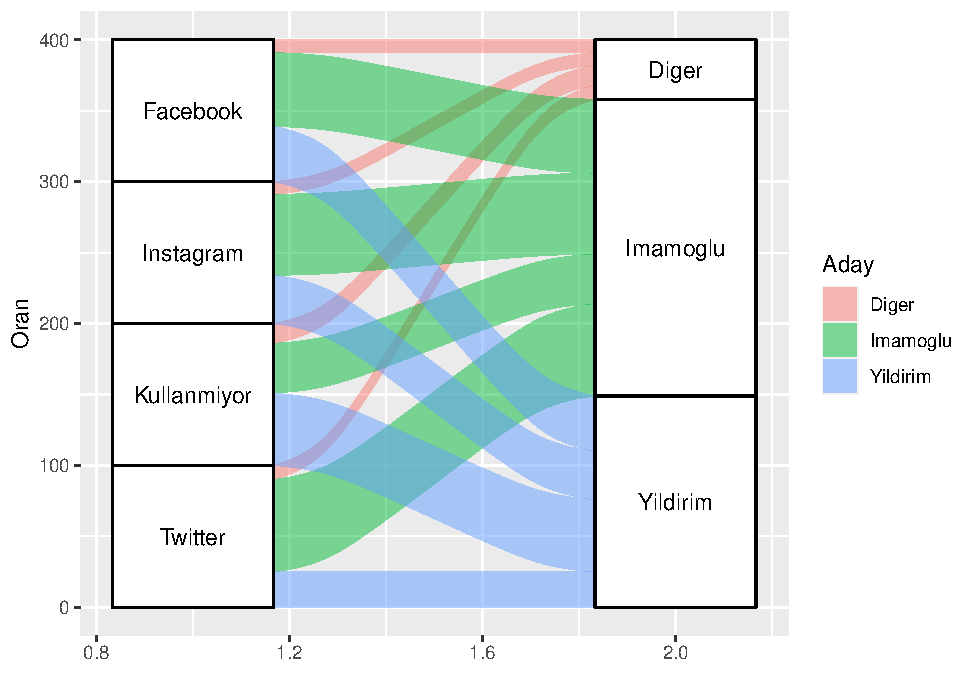
\includegraphics{rViz_files/figure-latex/unnamed-chunk-4-1.pdf}

\begin{itemize}
\item
  Kutuları küçültebiliriz.
\item
  Kutular ile yazıların renklerini değiştirebiliriz.
\item
  Geçiş renklerini değiştirebiliriz, şeffaflığını ayarlayabiliriz.
\item
  Boşlukları kapatabiliriz.
\item
  x eksenindeki isimleri değiştirebiliriz.
\item
  y eksenindeki değerleri kaldırabiliriz.
\end{itemize}

\begin{Shaded}
\begin{Highlighting}[]
\KeywordTok{ggplot}\NormalTok{(}\DataTypeTok{data =}\NormalTok{ v1, }\DataTypeTok{mapping =} \KeywordTok{aes}\NormalTok{(}\DataTypeTok{y =}\NormalTok{ Oran, }\DataTypeTok{axis1 =} \StringTok{`}\DataTypeTok{Sosyal Medya}\StringTok{`}\NormalTok{, }\DataTypeTok{axis2 =}\NormalTok{ Aday)) }\OperatorTok{+}
\StringTok{  }\KeywordTok{geom_alluvium}\NormalTok{(}\KeywordTok{aes}\NormalTok{(}\DataTypeTok{fill =}\NormalTok{ Aday), }\DataTypeTok{alpha =} \FloatTok{0.7}\NormalTok{) }\OperatorTok{+}
\StringTok{  }\KeywordTok{geom_stratum}\NormalTok{(}\DataTypeTok{width =} \FloatTok{0.2}\NormalTok{, }\DataTypeTok{fill =} \StringTok{"gray15"}\NormalTok{) }\OperatorTok{+}
\StringTok{  }\KeywordTok{geom_text}\NormalTok{(}\DataTypeTok{stat =} \StringTok{"stratum"}\NormalTok{, }\DataTypeTok{infer.label =} \OtherTok{TRUE}\NormalTok{, }\DataTypeTok{color =} \StringTok{"white"}\NormalTok{) }\OperatorTok{+}
\StringTok{  }\KeywordTok{scale_fill_manual}\NormalTok{(}\DataTypeTok{values =} \KeywordTok{c}\NormalTok{(}\StringTok{"gray"}\NormalTok{, }\StringTok{"darkred"}\NormalTok{, }\StringTok{"orange"}\NormalTok{)) }\OperatorTok{+}
\StringTok{  }\KeywordTok{scale_x_discrete}\NormalTok{(}\DataTypeTok{limits =} \KeywordTok{c}\NormalTok{(}\StringTok{"Sosyal Medya"}\NormalTok{,}\StringTok{"Aday"}\NormalTok{), }\DataTypeTok{expand =} \KeywordTok{c}\NormalTok{(}\DecValTok{0}\NormalTok{,}\DecValTok{0}\NormalTok{)) }\OperatorTok{+}
\StringTok{  }\KeywordTok{theme}\NormalTok{(}\DataTypeTok{axis.text.y =} \KeywordTok{element_blank}\NormalTok{())}
\end{Highlighting}
\end{Shaded}

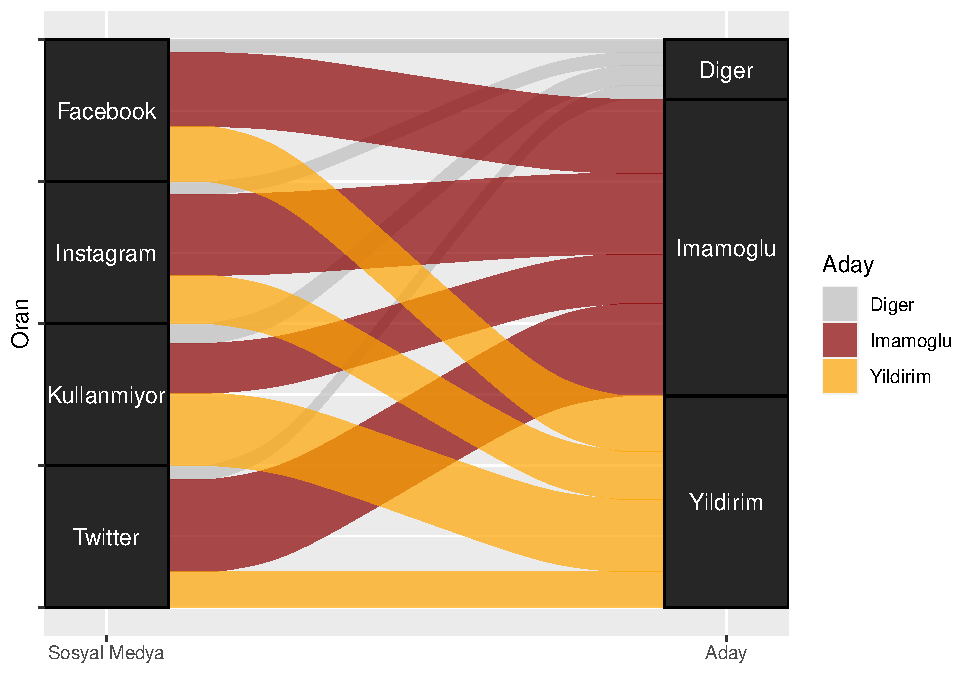
\includegraphics{rViz_files/figure-latex/unnamed-chunk-5-1.pdf}

\begin{itemize}
\item
  Lejantı düzenleyebiliriz.
\item
  y eksenine ait başlığı kaldırabiliriz.
\item
  Başlık ve kaynak ekleyebiliriz.
\item
  Temayı değiştirebiliriz.
\end{itemize}

\begin{Shaded}
\begin{Highlighting}[]
\KeywordTok{ggplot}\NormalTok{(}\DataTypeTok{data =}\NormalTok{ v1, }\DataTypeTok{mapping =} \KeywordTok{aes}\NormalTok{(}\DataTypeTok{y =}\NormalTok{ Oran, }\DataTypeTok{axis1 =} \StringTok{`}\DataTypeTok{Sosyal Medya}\StringTok{`}\NormalTok{, }\DataTypeTok{axis2 =}\NormalTok{ Aday)) }\OperatorTok{+}
\StringTok{  }\KeywordTok{geom_alluvium}\NormalTok{(}\KeywordTok{aes}\NormalTok{(}\DataTypeTok{fill =}\NormalTok{ Aday), }\DataTypeTok{alpha =} \FloatTok{0.7}\NormalTok{) }\OperatorTok{+}
\StringTok{  }\KeywordTok{geom_stratum}\NormalTok{(}\DataTypeTok{width =} \FloatTok{0.2}\NormalTok{, }\DataTypeTok{fill =} \StringTok{"gray15"}\NormalTok{) }\OperatorTok{+}
\StringTok{  }\KeywordTok{geom_text}\NormalTok{(}\DataTypeTok{stat =} \StringTok{"stratum"}\NormalTok{, }\DataTypeTok{infer.label =} \OtherTok{TRUE}\NormalTok{, }\DataTypeTok{color =} \StringTok{"white"}\NormalTok{) }\OperatorTok{+}
\StringTok{  }\KeywordTok{theme_void}\NormalTok{() }\OperatorTok{+}
\StringTok{  }\KeywordTok{scale_fill_manual}\NormalTok{(}\DataTypeTok{values =} \KeywordTok{c}\NormalTok{(}\StringTok{"gray"}\NormalTok{, }\StringTok{"darkred"}\NormalTok{, }\StringTok{"orange"}\NormalTok{)) }\OperatorTok{+}
\StringTok{  }\KeywordTok{scale_x_discrete}\NormalTok{(}\DataTypeTok{limits =} \KeywordTok{c}\NormalTok{(}\StringTok{"Sosyal Medya"}\NormalTok{,}\StringTok{"Aday"}\NormalTok{), }\DataTypeTok{expand =} \KeywordTok{c}\NormalTok{(}\DecValTok{0}\NormalTok{,}\DecValTok{0}\NormalTok{)) }\OperatorTok{+}
\StringTok{  }\KeywordTok{theme}\NormalTok{(}\DataTypeTok{plot.title =} \KeywordTok{element_text}\NormalTok{(}\DataTypeTok{hjust =} \FloatTok{0.5}\NormalTok{),}
        \DataTypeTok{axis.text.y =} \KeywordTok{element_blank}\NormalTok{(),}
        \DataTypeTok{legend.position =} \StringTok{"bottom"}\NormalTok{,}
        \DataTypeTok{legend.title =} \KeywordTok{element_blank}\NormalTok{()) }\OperatorTok{+}
\StringTok{  }\KeywordTok{labs}\NormalTok{(}\DataTypeTok{y =} \OtherTok{NULL}\NormalTok{,}
       \DataTypeTok{title =} \StringTok{"Sosyal Medya Kullanımına Göre İBB Aday Tercihi"}\NormalTok{,}
       \DataTypeTok{caption =} \StringTok{"Kaynak: Konda"}\NormalTok{)}
\end{Highlighting}
\end{Shaded}

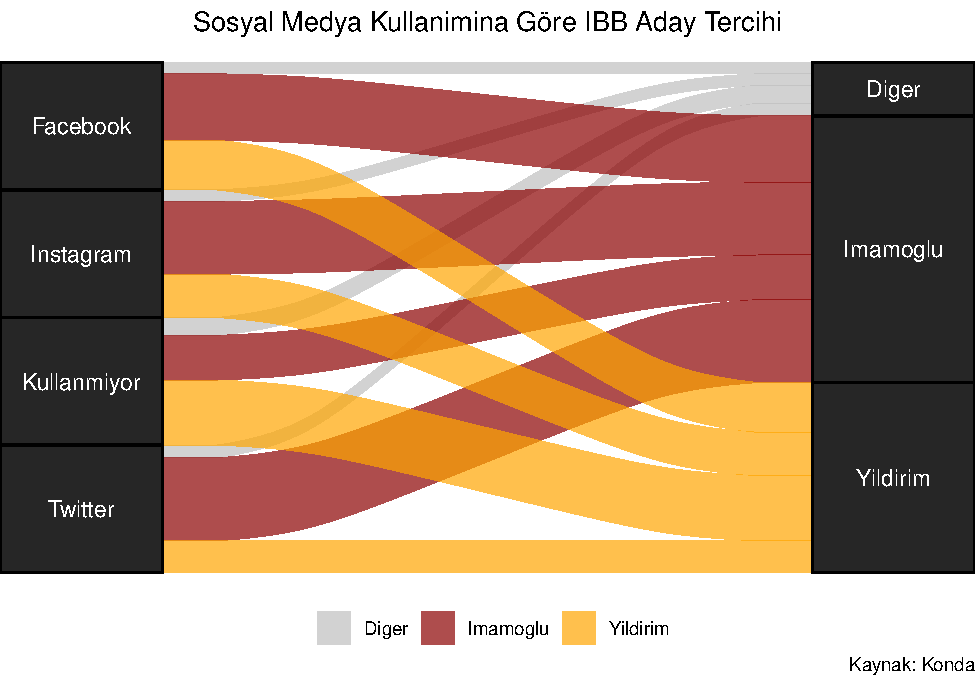
\includegraphics{rViz_files/figure-latex/unnamed-chunk-6-1.pdf}

\hypertarget{bar-uxe7ubuk}{%
\section{Bar (Çubuk)}\label{bar-uxe7ubuk}}

\emph{Bölgeler düzeyinde tiyatro seyirci sayısı:}

\begin{Shaded}
\begin{Highlighting}[]
\CommentTok{#En basit şekilde}

\KeywordTok{ggplot}\NormalTok{(}\DataTypeTok{data =}\NormalTok{ v2) }\OperatorTok{+}
\StringTok{  }\KeywordTok{geom_bar}\NormalTok{(}\DataTypeTok{mapping =} \KeywordTok{aes}\NormalTok{(}\DataTypeTok{x =} \StringTok{`}\DataTypeTok{Bölge}\StringTok{`}\NormalTok{, }\DataTypeTok{y =}\NormalTok{ Tiyatro), }\DataTypeTok{stat =} \StringTok{"identity"}\NormalTok{)}
\end{Highlighting}
\end{Shaded}

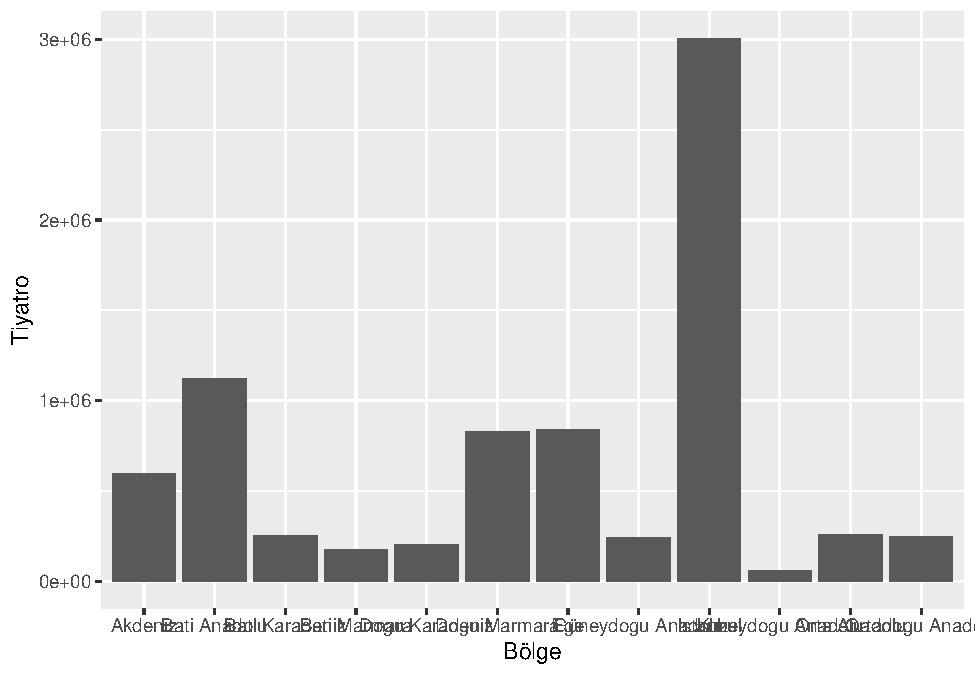
\includegraphics{rViz_files/figure-latex/unnamed-chunk-7-1.pdf}

\begin{Shaded}
\begin{Highlighting}[]
\CommentTok{#Alternatif}

\KeywordTok{ggplot}\NormalTok{(}\DataTypeTok{data =}\NormalTok{ v2) }\OperatorTok{+}
\StringTok{  }\KeywordTok{geom_col}\NormalTok{(}\DataTypeTok{mapping =} \KeywordTok{aes}\NormalTok{(}\DataTypeTok{x =} \StringTok{`}\DataTypeTok{Bölge}\StringTok{`}\NormalTok{, }\DataTypeTok{y =}\NormalTok{ Tiyatro))}
\end{Highlighting}
\end{Shaded}

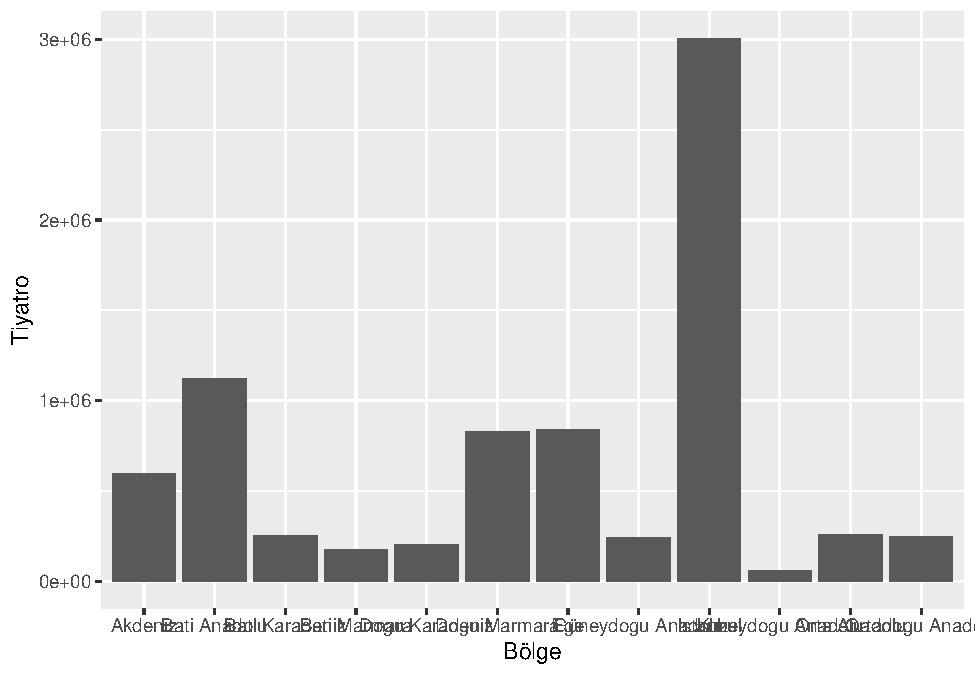
\includegraphics{rViz_files/figure-latex/unnamed-chunk-7-2.pdf}

\begin{itemize}
\item
  x ekseninde yer alan bölge isimlerini küçültebiliriz.
\item
  y eksenine ait değerleri daha okunabilir bir formata getirebiliriz.
\item
  Çubukları büyükten küçüğe doğru sıralayabiliriz.
\item
  Çubukları renklendirebiliriz.
\end{itemize}

\begin{Shaded}
\begin{Highlighting}[]
\KeywordTok{ggplot}\NormalTok{(}\DataTypeTok{data =}\NormalTok{ v2) }\OperatorTok{+}
\StringTok{  }\KeywordTok{geom_col}\NormalTok{(}\DataTypeTok{mapping =} \KeywordTok{aes}\NormalTok{(}\DataTypeTok{x =} \KeywordTok{reorder}\NormalTok{(}\StringTok{`}\DataTypeTok{Bölge}\StringTok{`}\NormalTok{, }\OperatorTok{-}\NormalTok{Tiyatro), }\DataTypeTok{y =}\NormalTok{ Tiyatro, }\DataTypeTok{fill =} \StringTok{`}\DataTypeTok{Bölge}\StringTok{`}\NormalTok{)) }\OperatorTok{+}
\StringTok{  }\KeywordTok{theme}\NormalTok{(}\DataTypeTok{axis.text.x =} \KeywordTok{element_text}\NormalTok{(}\DataTypeTok{size =} \DecValTok{5}\NormalTok{)) }\OperatorTok{+}
\StringTok{  }\KeywordTok{scale_y_continuous}\NormalTok{(}\DataTypeTok{labels =}\NormalTok{ comma)}
\end{Highlighting}
\end{Shaded}

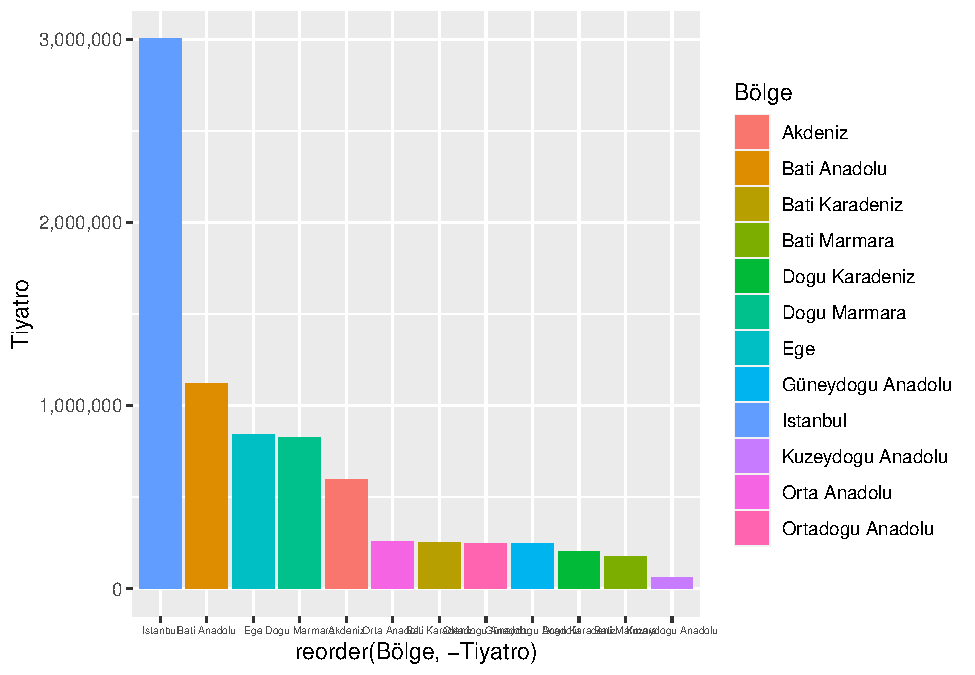
\includegraphics{rViz_files/figure-latex/unnamed-chunk-8-1.pdf}

\begin{itemize}
\item
  Lejantı kaldırabiliriz.
\item
  x ve y eksenlerine ait başlıkları kaldırabiliriz.
\item
  Başlık, alt başlık ve kaynak ekleyebiliriz.
\item
  Temayı değiştirebiliriz.
\end{itemize}

\begin{Shaded}
\begin{Highlighting}[]
\KeywordTok{ggplot}\NormalTok{(}\DataTypeTok{data =}\NormalTok{ v2) }\OperatorTok{+}
\StringTok{  }\KeywordTok{geom_col}\NormalTok{(}\DataTypeTok{mapping =} \KeywordTok{aes}\NormalTok{(}\DataTypeTok{x =} \KeywordTok{reorder}\NormalTok{(}\StringTok{`}\DataTypeTok{Bölge}\StringTok{`}\NormalTok{, }\OperatorTok{-}\StringTok{`}\DataTypeTok{Tiyatro}\StringTok{`}\NormalTok{), }\DataTypeTok{y =}\NormalTok{ Tiyatro, }\DataTypeTok{fill =} \StringTok{`}\DataTypeTok{Bölge}\StringTok{`}\NormalTok{)) }\OperatorTok{+}
\StringTok{  }\KeywordTok{theme_minimal}\NormalTok{() }\OperatorTok{+}
\StringTok{  }\KeywordTok{scale_y_continuous}\NormalTok{(}\DataTypeTok{labels =}\NormalTok{ comma) }\OperatorTok{+}
\StringTok{  }\KeywordTok{theme}\NormalTok{(}\DataTypeTok{axis.text.x =} \KeywordTok{element_text}\NormalTok{(}\DataTypeTok{size =} \DecValTok{6}\NormalTok{),}
        \DataTypeTok{axis.title.x =} \KeywordTok{element_blank}\NormalTok{(),}
        \DataTypeTok{axis.title.y =} \KeywordTok{element_blank}\NormalTok{(),}
        \DataTypeTok{legend.position =} \StringTok{"none"}\NormalTok{) }\OperatorTok{+}
\StringTok{  }\KeywordTok{labs}\NormalTok{(}\DataTypeTok{x =} \OtherTok{NULL}\NormalTok{,}
       \DataTypeTok{y =} \OtherTok{NULL}\NormalTok{,}
       \DataTypeTok{title =} \StringTok{"Bölgeler Düzeyinde Tiyatro Seyirci Sayısı"}\NormalTok{,}
       \DataTypeTok{subtitle =} \StringTok{"2018 yılına ait verilerdir"}\NormalTok{,}
       \DataTypeTok{caption =} \StringTok{"Kaynak: TÜİK"}\NormalTok{)}
\end{Highlighting}
\end{Shaded}

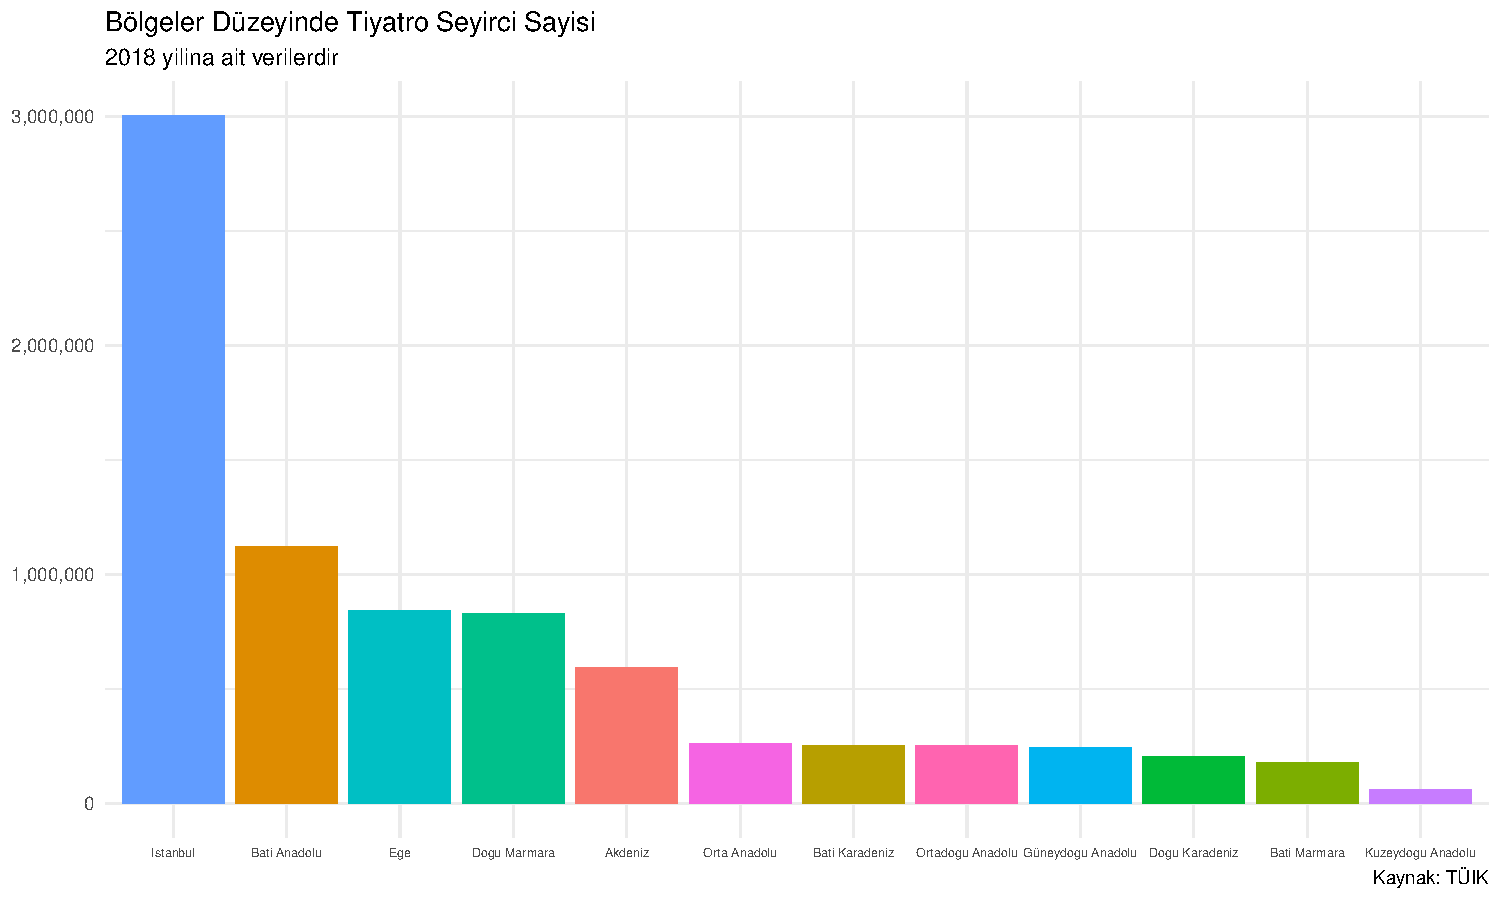
\includegraphics{rViz_files/figure-latex/unnamed-chunk-9-1.pdf}

\begin{itemize}
\tightlist
\item
  Çubukları yatay bir şekilde de gösterebiliriz.
\end{itemize}

\begin{Shaded}
\begin{Highlighting}[]
\KeywordTok{ggplot}\NormalTok{(}\DataTypeTok{data =}\NormalTok{ v2) }\OperatorTok{+}
\StringTok{  }\KeywordTok{geom_col}\NormalTok{(}\DataTypeTok{mapping =} \KeywordTok{aes}\NormalTok{(}\DataTypeTok{x =} \KeywordTok{reorder}\NormalTok{(}\StringTok{`}\DataTypeTok{Bölge}\StringTok{`}\NormalTok{, }\StringTok{`}\DataTypeTok{Tiyatro}\StringTok{`}\NormalTok{), }\DataTypeTok{y =}\NormalTok{ Tiyatro, }\DataTypeTok{fill =} \StringTok{`}\DataTypeTok{Bölge}\StringTok{`}\NormalTok{)) }\OperatorTok{+}
\StringTok{  }\KeywordTok{theme_minimal}\NormalTok{() }\OperatorTok{+}
\StringTok{  }\KeywordTok{scale_y_continuous}\NormalTok{(}\DataTypeTok{labels =}\NormalTok{ comma) }\OperatorTok{+}
\StringTok{  }\KeywordTok{theme}\NormalTok{(}\DataTypeTok{axis.title.x =} \KeywordTok{element_blank}\NormalTok{(),}
        \DataTypeTok{axis.title.y =} \KeywordTok{element_blank}\NormalTok{(),}
        \DataTypeTok{legend.position =} \StringTok{"none"}\NormalTok{) }\OperatorTok{+}
\StringTok{  }\KeywordTok{labs}\NormalTok{(}\DataTypeTok{x =} \OtherTok{NULL}\NormalTok{,}
       \DataTypeTok{y =} \OtherTok{NULL}\NormalTok{,}
       \DataTypeTok{title =} \StringTok{"Bölgeler Düzeyinde Tiyatro Seyirci Sayısı"}\NormalTok{,}
       \DataTypeTok{subtitle =} \StringTok{"2018 yılına ait verilerdir"}\NormalTok{,}
       \DataTypeTok{caption =} \StringTok{"Kaynak: TÜİK"}\NormalTok{) }\OperatorTok{+}
\StringTok{  }\KeywordTok{coord_flip}\NormalTok{()}
\end{Highlighting}
\end{Shaded}

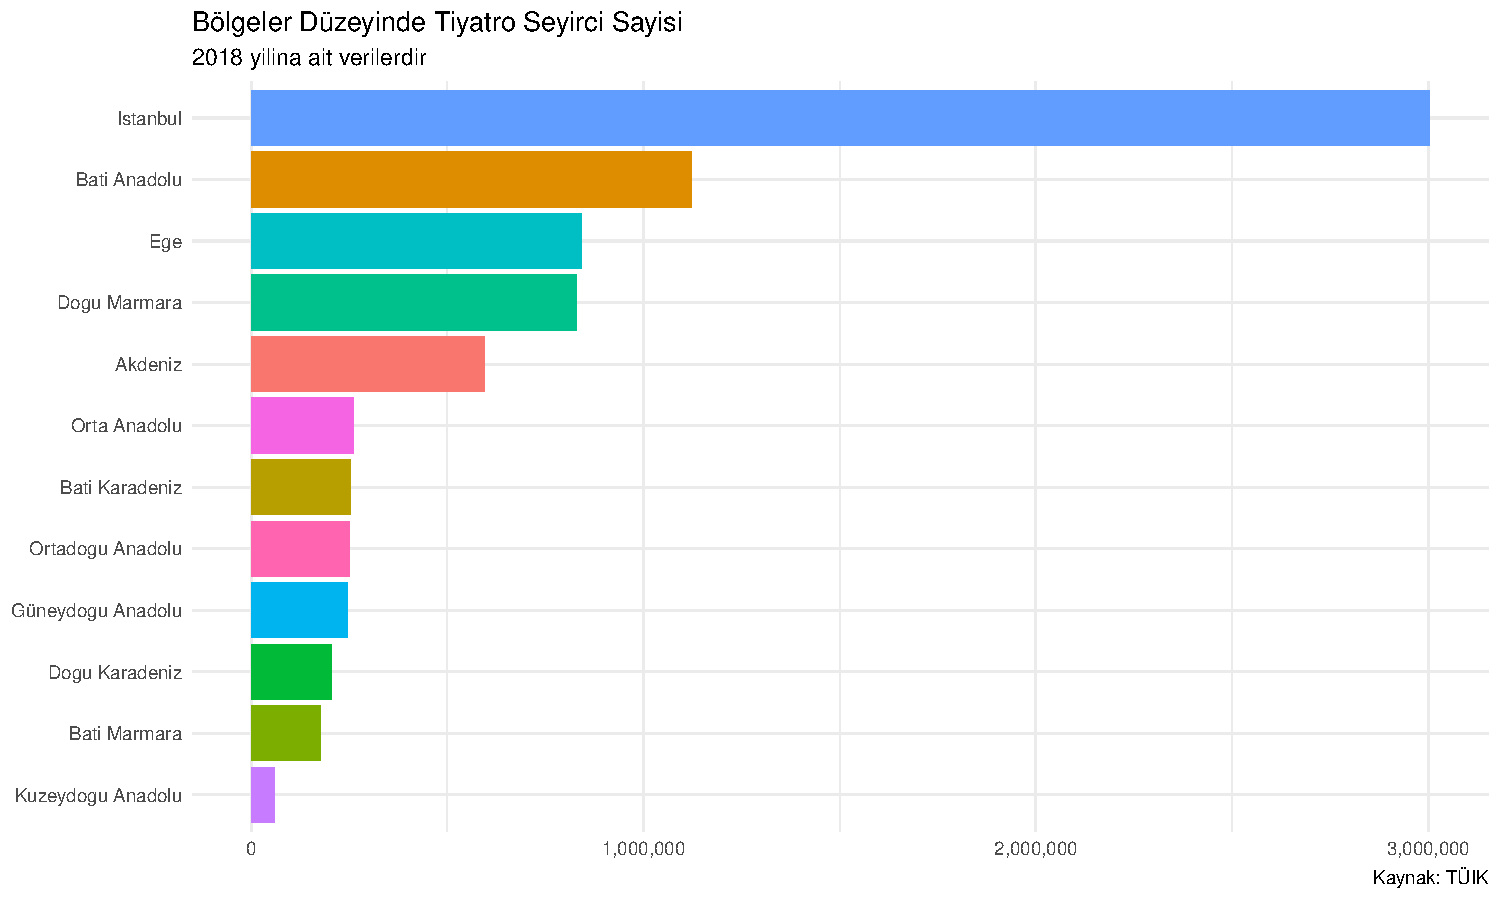
\includegraphics{rViz_files/figure-latex/unnamed-chunk-10-1.pdf}

\hypertarget{box-and-whisker-kutu-bux131yux131k}{%
\section{Box and Whisker (Kutu-Bıyık)}\label{box-and-whisker-kutu-bux131yux131k}}

\emph{Günlük BIST Hizmet, Mali, Sınai, Teknoloji endeks kapanışları:}

\begin{Shaded}
\begin{Highlighting}[]
\CommentTok{#En basit şekilde}

\KeywordTok{ggplot}\NormalTok{(}\DataTypeTok{data =}\NormalTok{ v3) }\OperatorTok{+}
\StringTok{  }\KeywordTok{geom_boxplot}\NormalTok{(}\DataTypeTok{mapping =} \KeywordTok{aes}\NormalTok{(}\DataTypeTok{x =}\NormalTok{ Endeks, }\DataTypeTok{y =} \StringTok{`}\DataTypeTok{Kapanış}\StringTok{`}\NormalTok{))}
\end{Highlighting}
\end{Shaded}

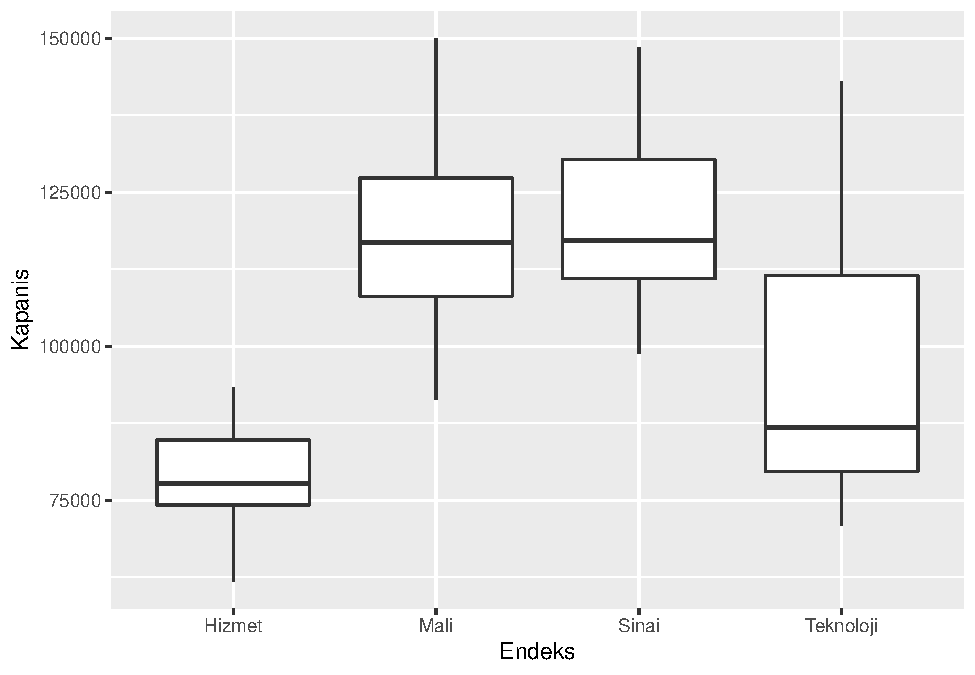
\includegraphics{rViz_files/figure-latex/unnamed-chunk-11-1.pdf}

\begin{itemize}
\item
  y eksenine ait değerleri daha okunabilir bir formata getirebiliriz.
\item
  Kutuları renklendirebiliriz.
\end{itemize}

\begin{Shaded}
\begin{Highlighting}[]
\KeywordTok{ggplot}\NormalTok{(}\DataTypeTok{data =}\NormalTok{ v3) }\OperatorTok{+}
\StringTok{  }\KeywordTok{geom_boxplot}\NormalTok{(}\DataTypeTok{mapping =} \KeywordTok{aes}\NormalTok{(}\DataTypeTok{x =}\NormalTok{ Endeks, }\DataTypeTok{y =} \StringTok{`}\DataTypeTok{Kapanış}\StringTok{`}\NormalTok{, }\DataTypeTok{fill =}\NormalTok{ Endeks)) }\OperatorTok{+}
\StringTok{  }\KeywordTok{scale_y_continuous}\NormalTok{(}\DataTypeTok{labels =}\NormalTok{ comma) }\OperatorTok{+}
\StringTok{  }\KeywordTok{scale_fill_brewer}\NormalTok{(}\DataTypeTok{palette =} \StringTok{"Set1"}\NormalTok{)}
\end{Highlighting}
\end{Shaded}

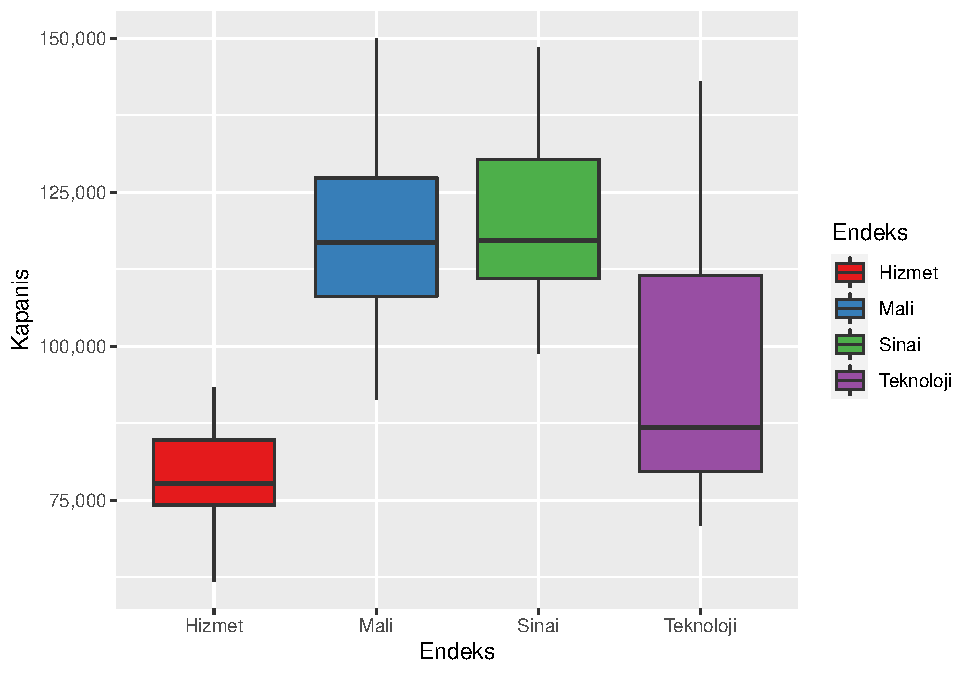
\includegraphics{rViz_files/figure-latex/unnamed-chunk-12-1.pdf}

\begin{itemize}
\item
  Lejantı kaldırabiliriz.
\item
  x eksenine ait başlığı kaldırabiliriz.
\item
  Başlık, alt başlık ve kaynak ekleyebiliriz.
\item
  Temayı değiştirebiliriz.
\end{itemize}

\begin{Shaded}
\begin{Highlighting}[]
\KeywordTok{ggplot}\NormalTok{(}\DataTypeTok{data =}\NormalTok{ v3) }\OperatorTok{+}
\StringTok{  }\KeywordTok{geom_boxplot}\NormalTok{(}\DataTypeTok{mapping =} \KeywordTok{aes}\NormalTok{(}\DataTypeTok{x =}\NormalTok{ Endeks, }\DataTypeTok{y =} \StringTok{`}\DataTypeTok{Kapanış}\StringTok{`}\NormalTok{, }\DataTypeTok{fill =}\NormalTok{ Endeks)) }\OperatorTok{+}
\StringTok{  }\KeywordTok{theme_minimal}\NormalTok{() }\OperatorTok{+}
\StringTok{  }\KeywordTok{scale_y_continuous}\NormalTok{(}\DataTypeTok{labels =}\NormalTok{ comma) }\OperatorTok{+}
\StringTok{  }\KeywordTok{scale_fill_brewer}\NormalTok{(}\DataTypeTok{palette =} \StringTok{"Set1"}\NormalTok{) }\OperatorTok{+}
\StringTok{  }\KeywordTok{theme}\NormalTok{(}\DataTypeTok{legend.position =} \StringTok{"none"}\NormalTok{) }\OperatorTok{+}
\StringTok{  }\KeywordTok{labs}\NormalTok{(}\DataTypeTok{x =} \OtherTok{NULL}\NormalTok{,}
       \DataTypeTok{title =} \StringTok{"Günlük BIST Hizmet, Mali, Sınai, Teknoloji Endeks Kapanışları"}\NormalTok{,}
       \DataTypeTok{subtitle =} \StringTok{"Son 1 yıla ait verilerdir"}\NormalTok{,}
       \DataTypeTok{caption =} \StringTok{"Kaynak: TCMB"}\NormalTok{)}
\end{Highlighting}
\end{Shaded}

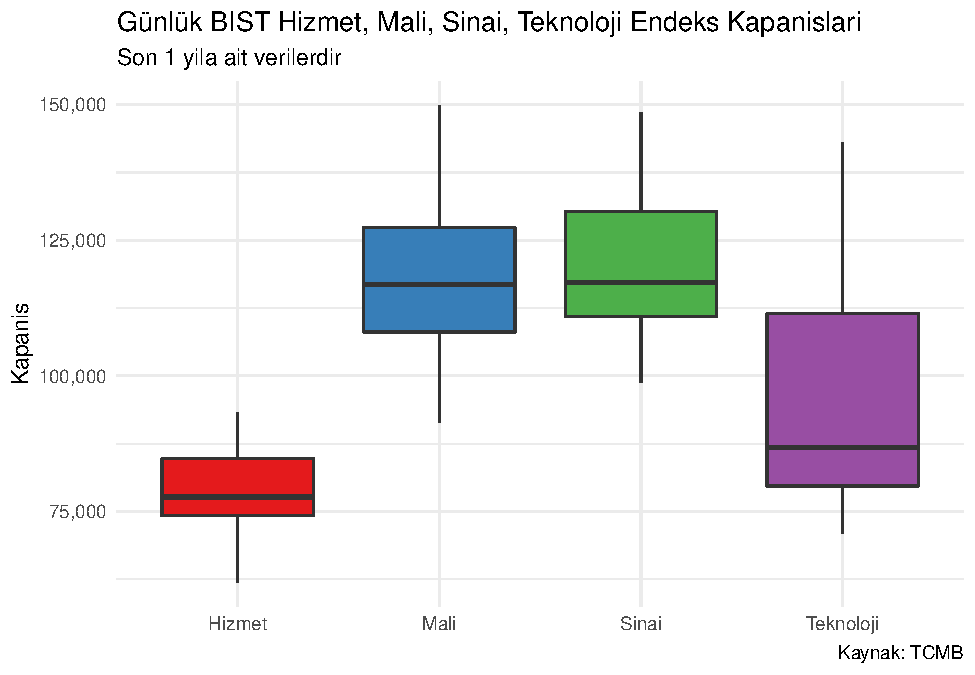
\includegraphics{rViz_files/figure-latex/unnamed-chunk-13-1.pdf}

\hypertarget{bubble-balon}{%
\section{Bubble (Balon)}\label{bubble-balon}}

\emph{İl ve ilçelere göre İnsani Gelişme Endeksi:}

\begin{Shaded}
\begin{Highlighting}[]
\CommentTok{#En basit şekilde}

\KeywordTok{ggplot}\NormalTok{(}\DataTypeTok{data =}\NormalTok{ v4) }\OperatorTok{+}
\StringTok{  }\KeywordTok{geom_point}\NormalTok{(}\DataTypeTok{mapping =} \KeywordTok{aes}\NormalTok{(}\DataTypeTok{x =} \StringTok{`}\DataTypeTok{Nüfus`, y = Endeks, size = }\StringTok{`}\NormalTok{Nüfus`))}
\end{Highlighting}
\end{Shaded}

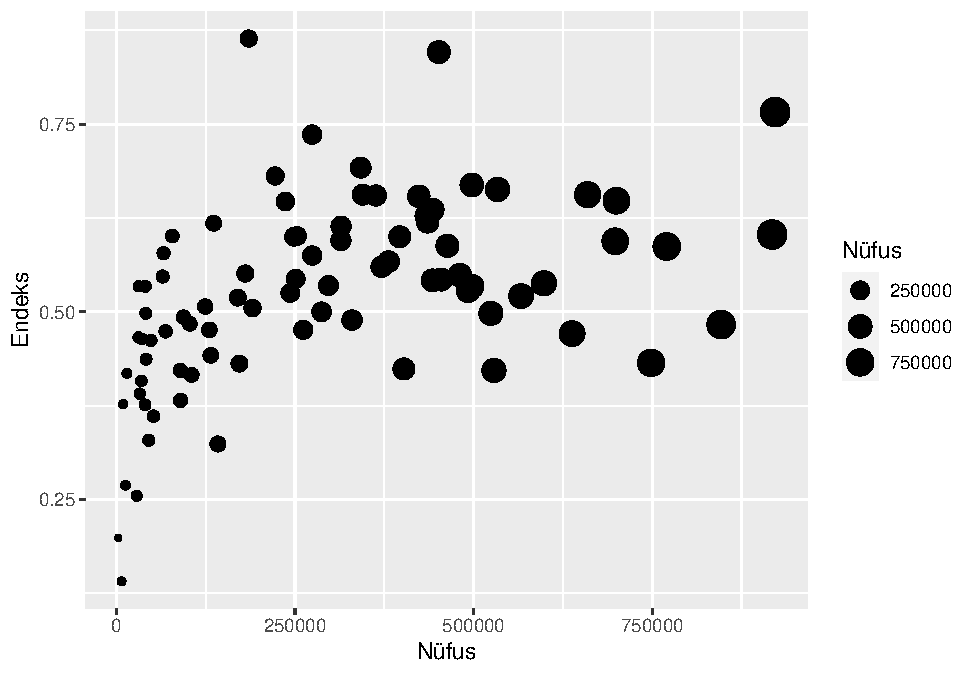
\includegraphics{rViz_files/figure-latex/unnamed-chunk-14-1.pdf}

\begin{itemize}
\item
  İllere göre renklendirebiliriz.
\item
  Noktaları düzenleyebiliriz.
\end{itemize}

\begin{Shaded}
\begin{Highlighting}[]
\KeywordTok{ggplot}\NormalTok{(}\DataTypeTok{data =}\NormalTok{ v4) }\OperatorTok{+}
\StringTok{  }\KeywordTok{geom_point}\NormalTok{(}\DataTypeTok{mapping =} \KeywordTok{aes}\NormalTok{(}\DataTypeTok{x =} \StringTok{`}\DataTypeTok{Nüfus`, y = Endeks, size = }\StringTok{`}\NormalTok{Nüfus`, }\DataTypeTok{fill =} \StringTok{`}\DataTypeTok{İl}\StringTok{`}\NormalTok{), }\DataTypeTok{alpha =} \FloatTok{0.5}\NormalTok{, }\DataTypeTok{shape =} \DecValTok{21}\NormalTok{) }\OperatorTok{+}
\StringTok{  }\KeywordTok{scale_color_viridis_d}\NormalTok{(}\DataTypeTok{option =} \StringTok{"A"}\NormalTok{)}
\end{Highlighting}
\end{Shaded}

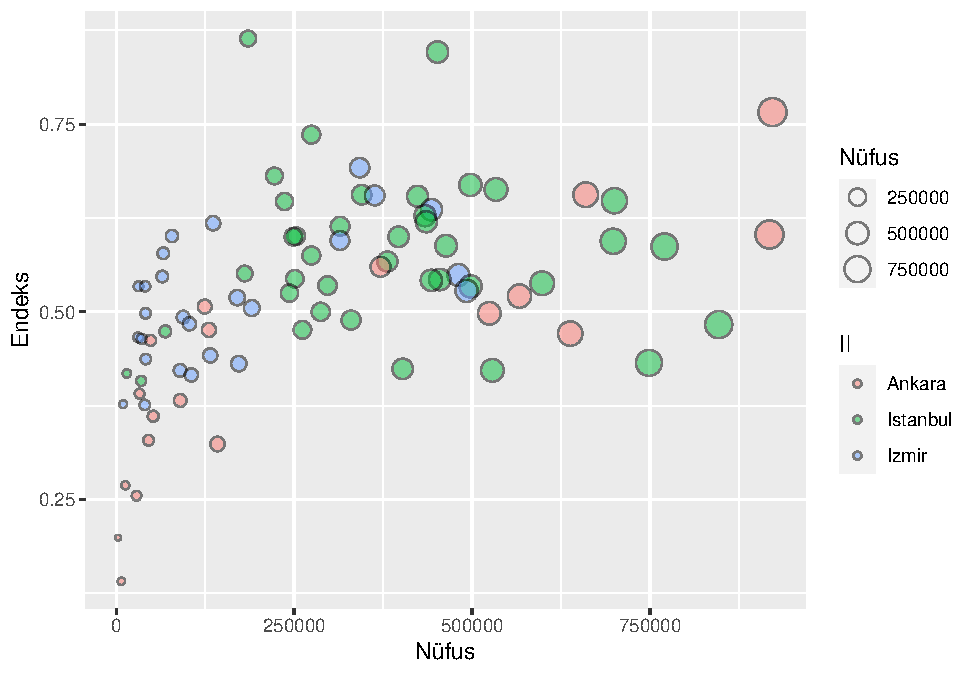
\includegraphics{rViz_files/figure-latex/unnamed-chunk-15-1.pdf}

\begin{itemize}
\item
  Lejantı düzenleyebiliriz.
\item
  x ve y eksenlerine ait başlıkları düzeltebiliriz.
\item
  Başlık, alt başlık ve kaynak ekleyebiliriz.
\item
  Temayı değiştirebiliriz.
\end{itemize}

\begin{Shaded}
\begin{Highlighting}[]
\KeywordTok{ggplot}\NormalTok{(}\DataTypeTok{data =}\NormalTok{ v4) }\OperatorTok{+}
\StringTok{  }\KeywordTok{geom_point}\NormalTok{(}\DataTypeTok{mapping =} \KeywordTok{aes}\NormalTok{(}\DataTypeTok{x =} \StringTok{`}\DataTypeTok{Nüfus`, y = Endeks, size = }\StringTok{`}\NormalTok{Nüfus`, }\DataTypeTok{fill =} \StringTok{`}\DataTypeTok{İl}\StringTok{`}\NormalTok{), }\DataTypeTok{alpha =} \FloatTok{0.5}\NormalTok{, }\DataTypeTok{shape =} \DecValTok{21}\NormalTok{) }\OperatorTok{+}
\StringTok{  }\KeywordTok{theme_fivethirtyeight}\NormalTok{() }\OperatorTok{+}
\StringTok{  }\KeywordTok{scale_fill_viridis_d}\NormalTok{() }\OperatorTok{+}
\StringTok{  }\KeywordTok{theme}\NormalTok{(}\DataTypeTok{legend.title =} \KeywordTok{element_blank}\NormalTok{(),}
        \DataTypeTok{legend.position =} \StringTok{"right"}\NormalTok{,}
        \DataTypeTok{legend.direction =} \StringTok{"vertical"}\NormalTok{,}
        \DataTypeTok{axis.title =} \KeywordTok{element_text}\NormalTok{()) }\OperatorTok{+}
\StringTok{  }\KeywordTok{labs}\NormalTok{(}\DataTypeTok{x =} \StringTok{"Nüfus",}
\StringTok{       y = "}\NormalTok{İnsani Gelişme Endeksi}\StringTok{",}
\StringTok{       title = "}\NormalTok{İl ve İlçelere Göre İnsani Gelişme Endeksi}\StringTok{",}
\StringTok{       caption = "}\NormalTok{Kaynak}\OperatorTok{:}\StringTok{ }\NormalTok{İnsani Gelişme Vakfı, TÜİK}\StringTok{")}
\end{Highlighting}
\end{Shaded}

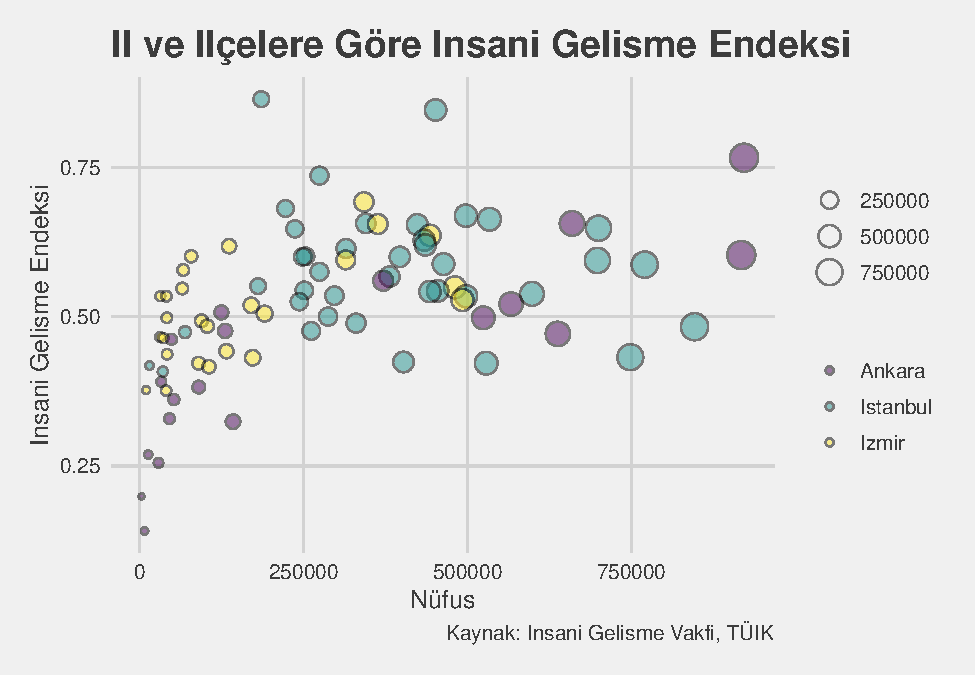
\includegraphics{rViz_files/figure-latex/unnamed-chunk-16-1.pdf}

\hypertarget{bubble-map-balon-harita}{%
\section{Bubble Map (Balon Harita)}\label{bubble-map-balon-harita}}

\emph{2017 yılında kaydedilen terörist saldırılar ve ölü sayısı (GTD):}

\begin{Shaded}
\begin{Highlighting}[]
\NormalTok{palet <-}\StringTok{ }\KeywordTok{colorFactor}\NormalTok{(}\DataTypeTok{palette =} \KeywordTok{c}\NormalTok{(}\StringTok{"blue"}\NormalTok{,}\StringTok{"yellow"}\NormalTok{,}\StringTok{"white"}\NormalTok{,}\StringTok{"red"}\NormalTok{,}\StringTok{"green"}\NormalTok{,}\StringTok{"purple"}\NormalTok{),}
                     \DataTypeTok{domain =}\NormalTok{ v5}\OperatorTok{$}\NormalTok{Grup) }\CommentTok{#Renk ayarları}

\NormalTok{v5 }\OperatorTok\StringTok{ }
\StringTok{  }\KeywordTok{leaflet}\NormalTok{() }\OperatorTok\StringTok{ }
\StringTok{  }\KeywordTok{addTiles}\NormalTok{() }\OperatorTok
\StringTok{  }\KeywordTok{addProviderTiles}\NormalTok{(}\DataTypeTok{provider =}\NormalTok{ providers}\OperatorTok{$}\NormalTok{CartoDB.DarkMatterNoLabels) }\OperatorTok\StringTok{ }\CommentTok{#Harita tipi}
\StringTok{  }\KeywordTok{addCircles}\NormalTok{(}\DataTypeTok{lng =} \OperatorTok{~}\NormalTok{Boylam, }\DataTypeTok{lat =} \OperatorTok{~}\NormalTok{Enlem, }\DataTypeTok{radius =} \OperatorTok{~}\StringTok{`}\DataTypeTok{Ölü Sayısı}\StringTok{`}\OperatorTok{*}\DecValTok{5000}\NormalTok{, }\DataTypeTok{stroke =} \OtherTok{FALSE}\NormalTok{, }\DataTypeTok{color =} \OperatorTok{~}\KeywordTok{palet}\NormalTok{(Grup)) }\OperatorTok\StringTok{ }
\StringTok{  }\KeywordTok{addLegend}\NormalTok{(}\DataTypeTok{position =} \StringTok{"bottomright"}\NormalTok{, }\DataTypeTok{pal =}\NormalTok{ palet, }\DataTypeTok{values =}\NormalTok{ v5}\OperatorTok{$}\NormalTok{Grup, }\DataTypeTok{title =} \StringTok{""}\NormalTok{, }\DataTypeTok{opacity =} \DecValTok{1}\NormalTok{) }\CommentTok{#Lejant}
\end{Highlighting}
\end{Shaded}

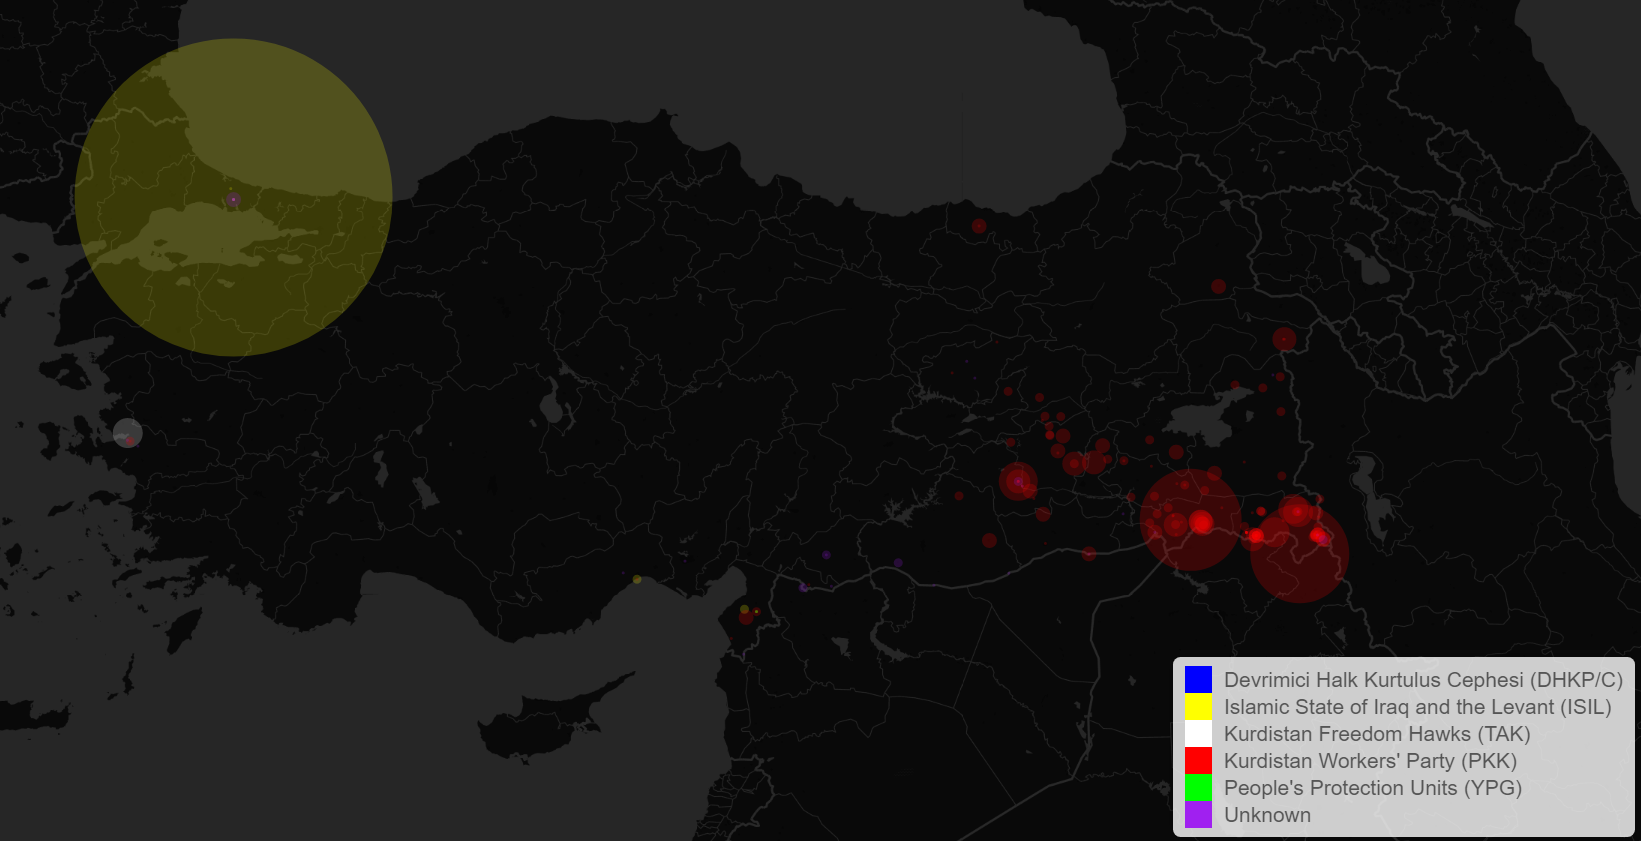
\includegraphics[width=1\linewidth]{C:/Users/datanerd/Desktop/Github/rViz/img/bubble}

\hypertarget{candlestick-mum}{%
\section{Candlestick (Mum)}\label{candlestick-mum}}

\emph{BIST'e ait açılış, en yüksek, en düşük, kapanış değerleri:}

\begin{Shaded}
\begin{Highlighting}[]
\NormalTok{v6 }\OperatorTok\StringTok{ }
\StringTok{  }\KeywordTok{mutate}\NormalTok{(}\DataTypeTok{Date =} \KeywordTok{ymd}\NormalTok{(Date))}

\CommentTok{#Veriler aşağıdaki gibi de alınabilir:}
\CommentTok{#tq_get(x = "GARAN.IS", from = "2020-05-04", to = "2020-05-20")}

\CommentTok{#En basit şekilde}

\KeywordTok{ggplot}\NormalTok{(}\DataTypeTok{data =}\NormalTok{ v6, }\DataTypeTok{mapping =} \KeywordTok{aes}\NormalTok{(}\DataTypeTok{x =}\NormalTok{ Date, }\DataTypeTok{y =}\NormalTok{ Close)) }\OperatorTok{+}
\StringTok{  }\KeywordTok{geom_candlestick}\NormalTok{(}\DataTypeTok{mapping =} \KeywordTok{aes}\NormalTok{(}\DataTypeTok{open =}\NormalTok{ Open, }\DataTypeTok{high =}\NormalTok{ High, }\DataTypeTok{low =}\NormalTok{ Low, }\DataTypeTok{close =}\NormalTok{ Close))}
\end{Highlighting}
\end{Shaded}

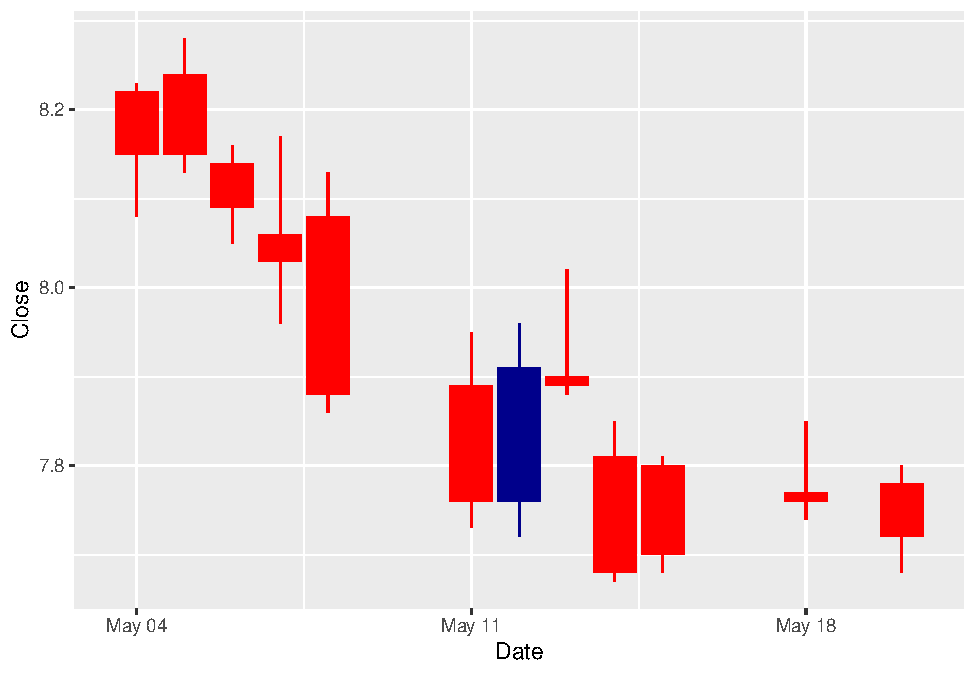
\includegraphics{rViz_files/figure-latex/unnamed-chunk-19-1.pdf}

\begin{itemize}
\tightlist
\item
  Düşüş ve yükseliş renklerini değiştirebiliriz.
\end{itemize}

\begin{Shaded}
\begin{Highlighting}[]
\KeywordTok{ggplot}\NormalTok{(}\DataTypeTok{data =}\NormalTok{ v6, }\DataTypeTok{mapping =} \KeywordTok{aes}\NormalTok{(}\DataTypeTok{x =}\NormalTok{ Date, }\DataTypeTok{y =}\NormalTok{ Close)) }\OperatorTok{+}
\StringTok{  }\KeywordTok{geom_candlestick}\NormalTok{(}\DataTypeTok{mapping =} \KeywordTok{aes}\NormalTok{(}\DataTypeTok{open =}\NormalTok{ Open, }\DataTypeTok{high =}\NormalTok{ High, }\DataTypeTok{low =}\NormalTok{ Low, }\DataTypeTok{close =}\NormalTok{ Close),}
                   \DataTypeTok{colour_up =} \StringTok{"darkgreen"}\NormalTok{, }\DataTypeTok{fill_up =} \StringTok{"darkgreen"}\NormalTok{,}
                   \DataTypeTok{colour_down =} \StringTok{"darkred"}\NormalTok{, }\DataTypeTok{fill_down =} \StringTok{"darkred"}\NormalTok{)}
\end{Highlighting}
\end{Shaded}

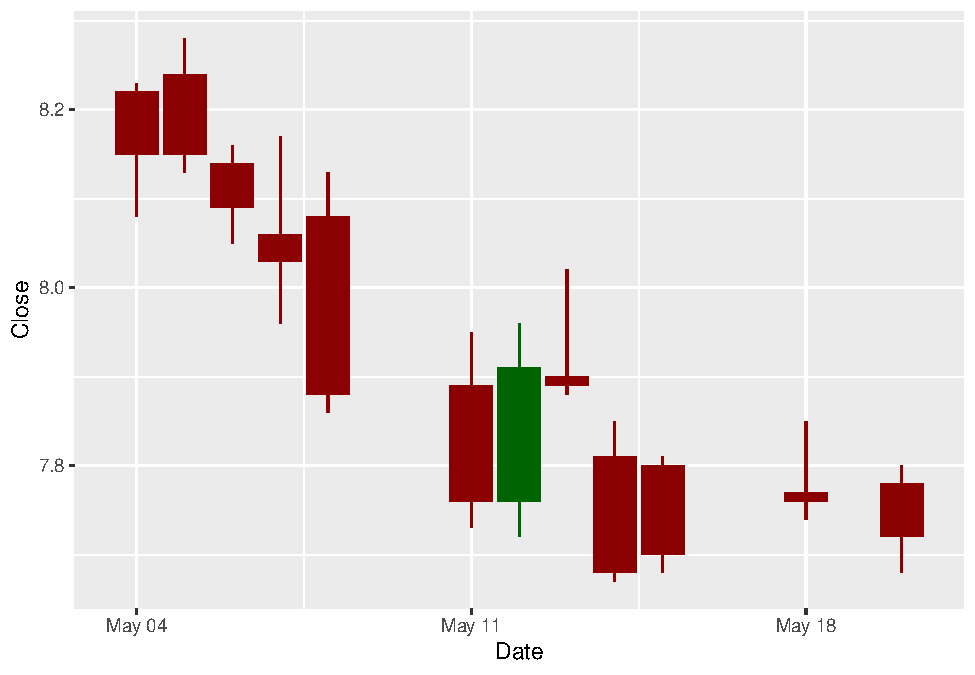
\includegraphics{rViz_files/figure-latex/unnamed-chunk-20-1.pdf}

\begin{itemize}
\item
  x ve y eksenlerine ait başlıkları kaldırabiliriz.
\item
  Başlık, alt başlık ve kaynak ekleyebiliriz.
\item
  Temayı değiştirebiliriz.
\end{itemize}

\begin{Shaded}
\begin{Highlighting}[]
\KeywordTok{ggplot}\NormalTok{(}\DataTypeTok{data =}\NormalTok{ v6, }\DataTypeTok{mapping =} \KeywordTok{aes}\NormalTok{(}\DataTypeTok{x =}\NormalTok{ Date, }\DataTypeTok{y =}\NormalTok{ Close)) }\OperatorTok{+}
\StringTok{  }\KeywordTok{geom_candlestick}\NormalTok{(}\DataTypeTok{mapping =} \KeywordTok{aes}\NormalTok{(}\DataTypeTok{open =}\NormalTok{ Open, }\DataTypeTok{high =}\NormalTok{ High, }\DataTypeTok{low =}\NormalTok{ Low, }\DataTypeTok{close =}\NormalTok{ Close),}
                   \DataTypeTok{colour_up =} \StringTok{"darkgreen"}\NormalTok{, }\DataTypeTok{fill_up =} \StringTok{"darkgreen"}\NormalTok{,}
                   \DataTypeTok{colour_down =} \StringTok{"darkred"}\NormalTok{, }\DataTypeTok{fill_down =} \StringTok{"darkred"}\NormalTok{) }\OperatorTok{+}
\StringTok{  }\KeywordTok{theme_tq}\NormalTok{() }\OperatorTok{+}
\StringTok{  }\KeywordTok{labs}\NormalTok{(}\DataTypeTok{x =} \OtherTok{NULL}\NormalTok{,}
       \DataTypeTok{y =} \OtherTok{NULL}\NormalTok{,}
       \DataTypeTok{title =} \StringTok{"Garanti Bankası Açılış, En Yüksek, En Düşük, Kapanış Değerleri"}\NormalTok{,}
       \DataTypeTok{subtitle =} \StringTok{"04.05.2020-20.05.2020"}\NormalTok{,}
       \DataTypeTok{caption =} \StringTok{"Kaynak: Yahoo"}\NormalTok{)}
\end{Highlighting}
\end{Shaded}

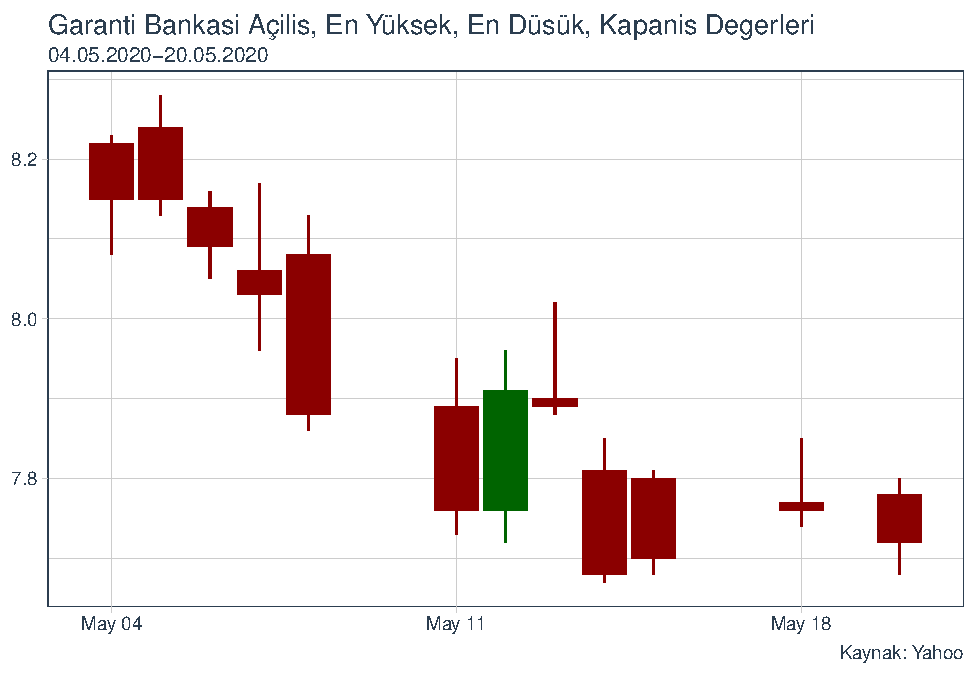
\includegraphics{rViz_files/figure-latex/unnamed-chunk-21-1.pdf}

\hypertarget{chord-akor}{%
\section{Chord (Akor)}\label{chord-akor}}

\emph{İstanbul, İzmir ve Ankara'nın en çok göç aldığı 5 il:}

\begin{Shaded}
\begin{Highlighting}[]
\CommentTok{#En basit şekilde}

\KeywordTok{chordDiagram}\NormalTok{(}\DataTypeTok{x =}\NormalTok{ v7) }\CommentTok{#GA: Göç Alan, GV: Göç veren}
\end{Highlighting}
\end{Shaded}

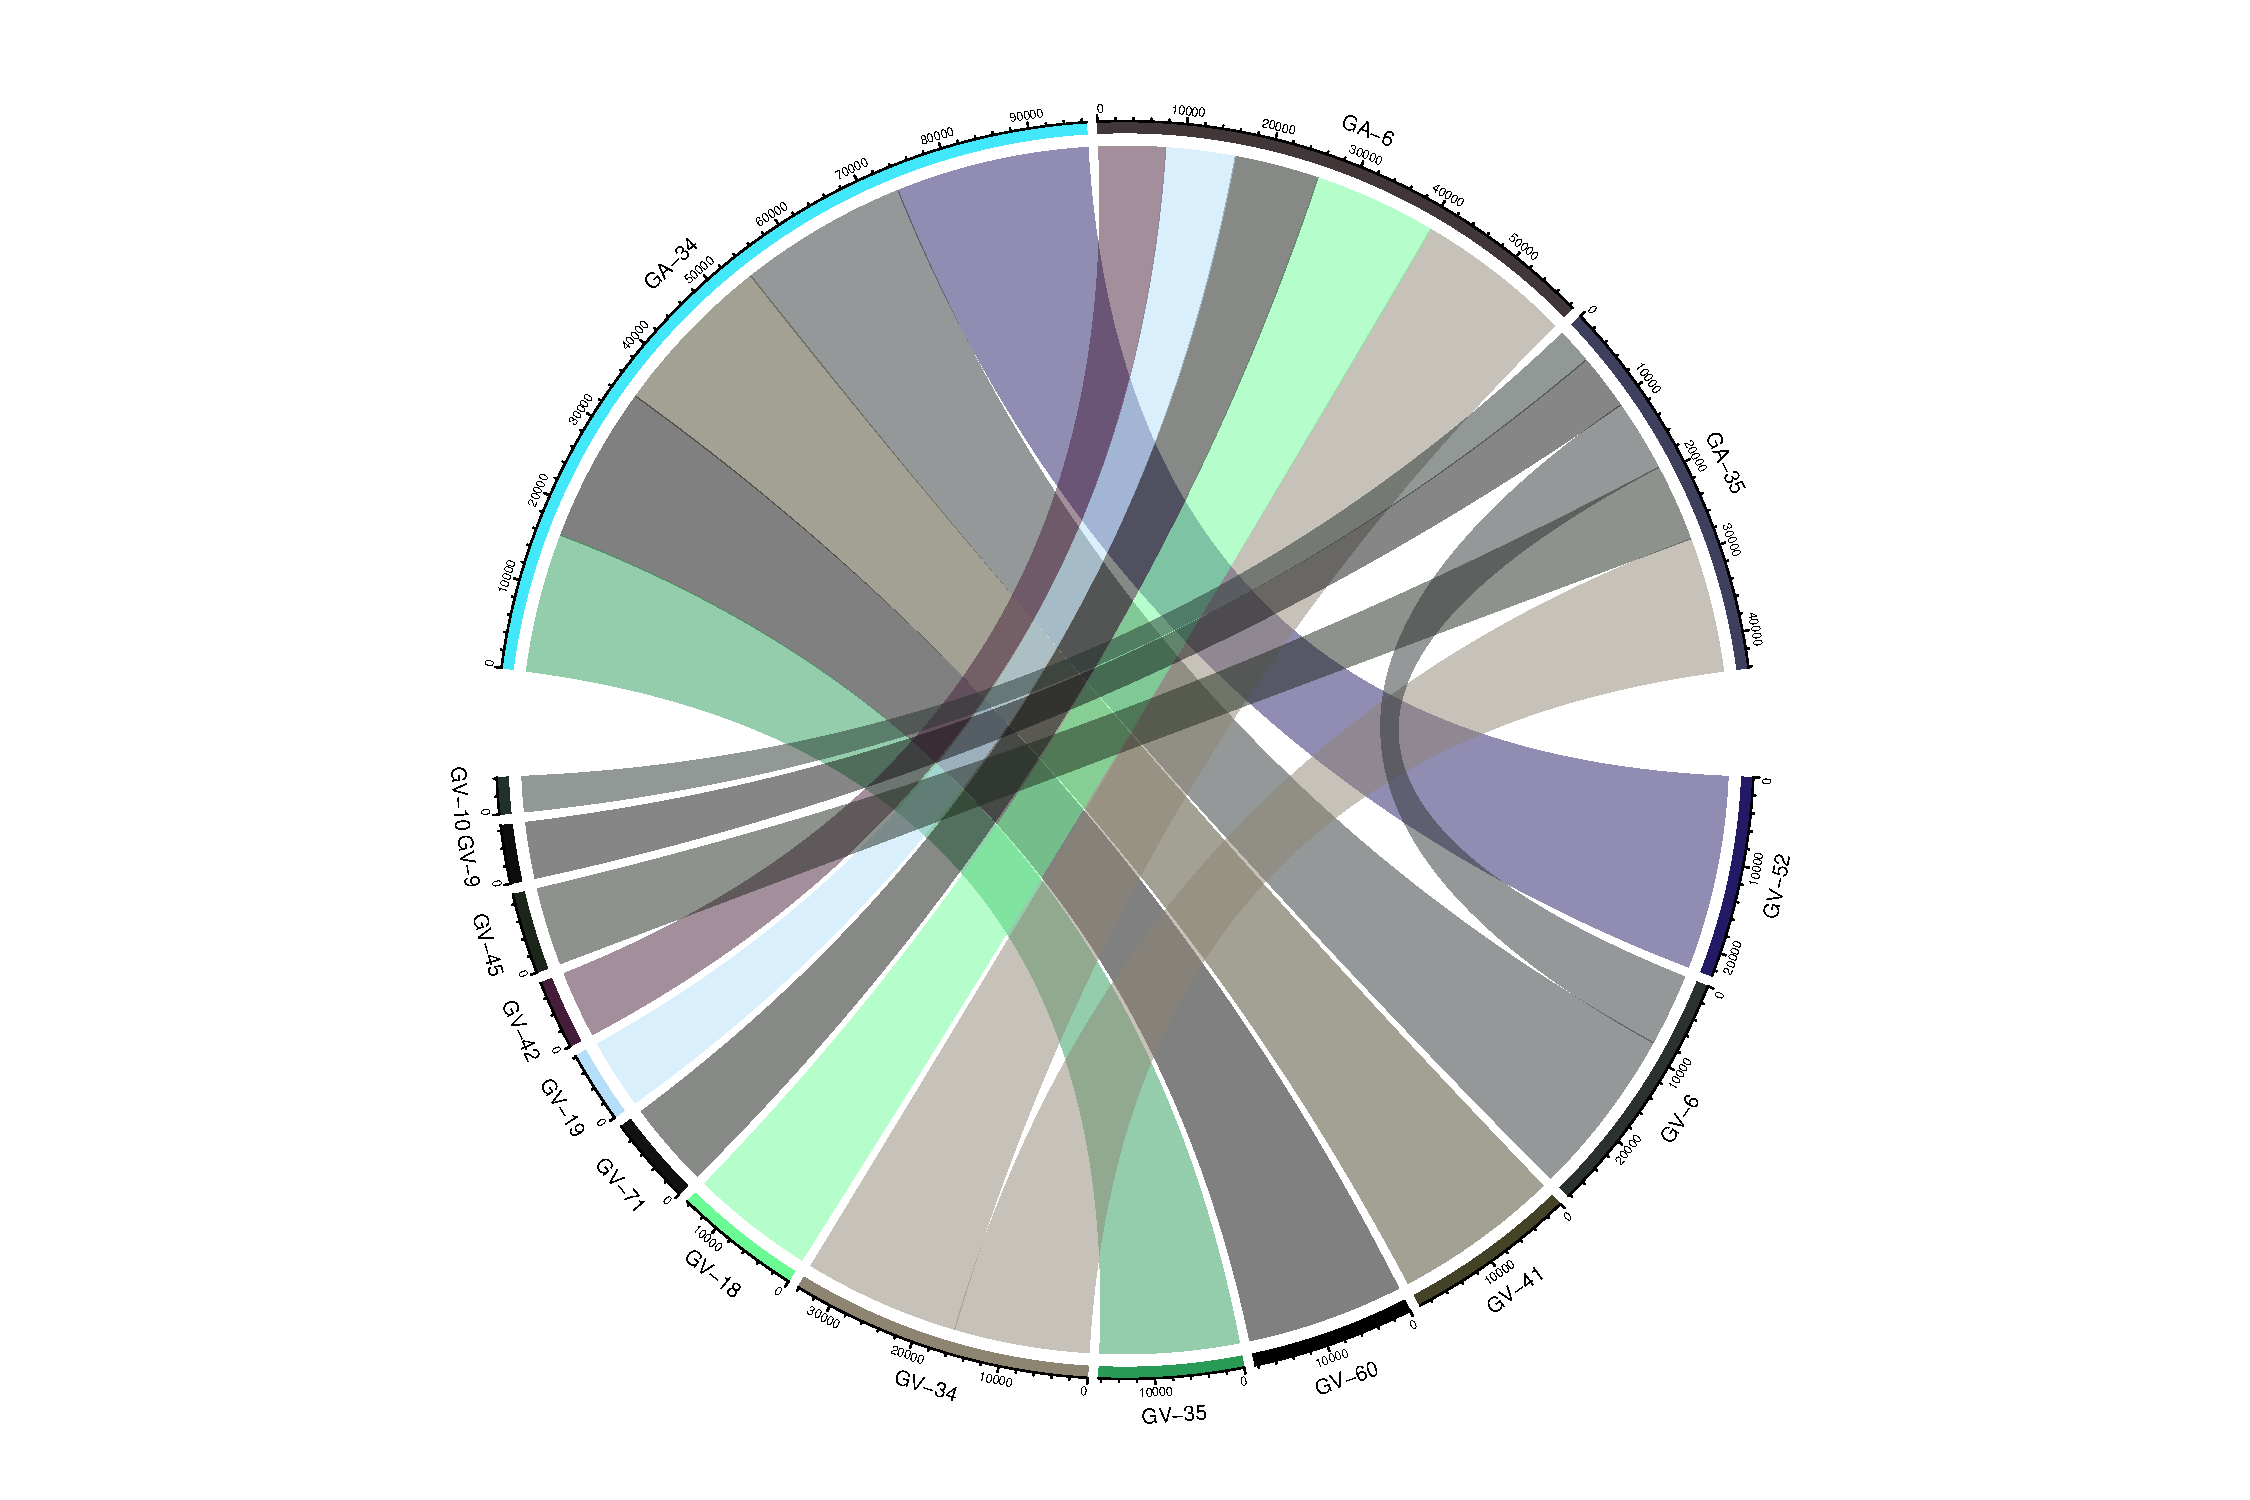
\includegraphics{rViz_files/figure-latex/unnamed-chunk-22-1.pdf}

\begin{itemize}
\tightlist
\item
  Renkleri değiştirebiliriz.
\end{itemize}

\begin{Shaded}
\begin{Highlighting}[]
\NormalTok{renkler <-}\StringTok{ }\KeywordTok{c}\NormalTok{(}\StringTok{`}\DataTypeTok{GA-34}\StringTok{`}\NormalTok{ =}\StringTok{ "red"}\NormalTok{, }\StringTok{`}\DataTypeTok{GA-6}\StringTok{`}\NormalTok{ =}\StringTok{ "orange"}\NormalTok{, }\StringTok{`}\DataTypeTok{GA-35}\StringTok{`}\NormalTok{ =}\StringTok{ "blue"}\NormalTok{)}

\KeywordTok{chordDiagram}\NormalTok{(}\DataTypeTok{x =}\NormalTok{ v7, }\DataTypeTok{col =}\NormalTok{ renkler)}
\end{Highlighting}
\end{Shaded}

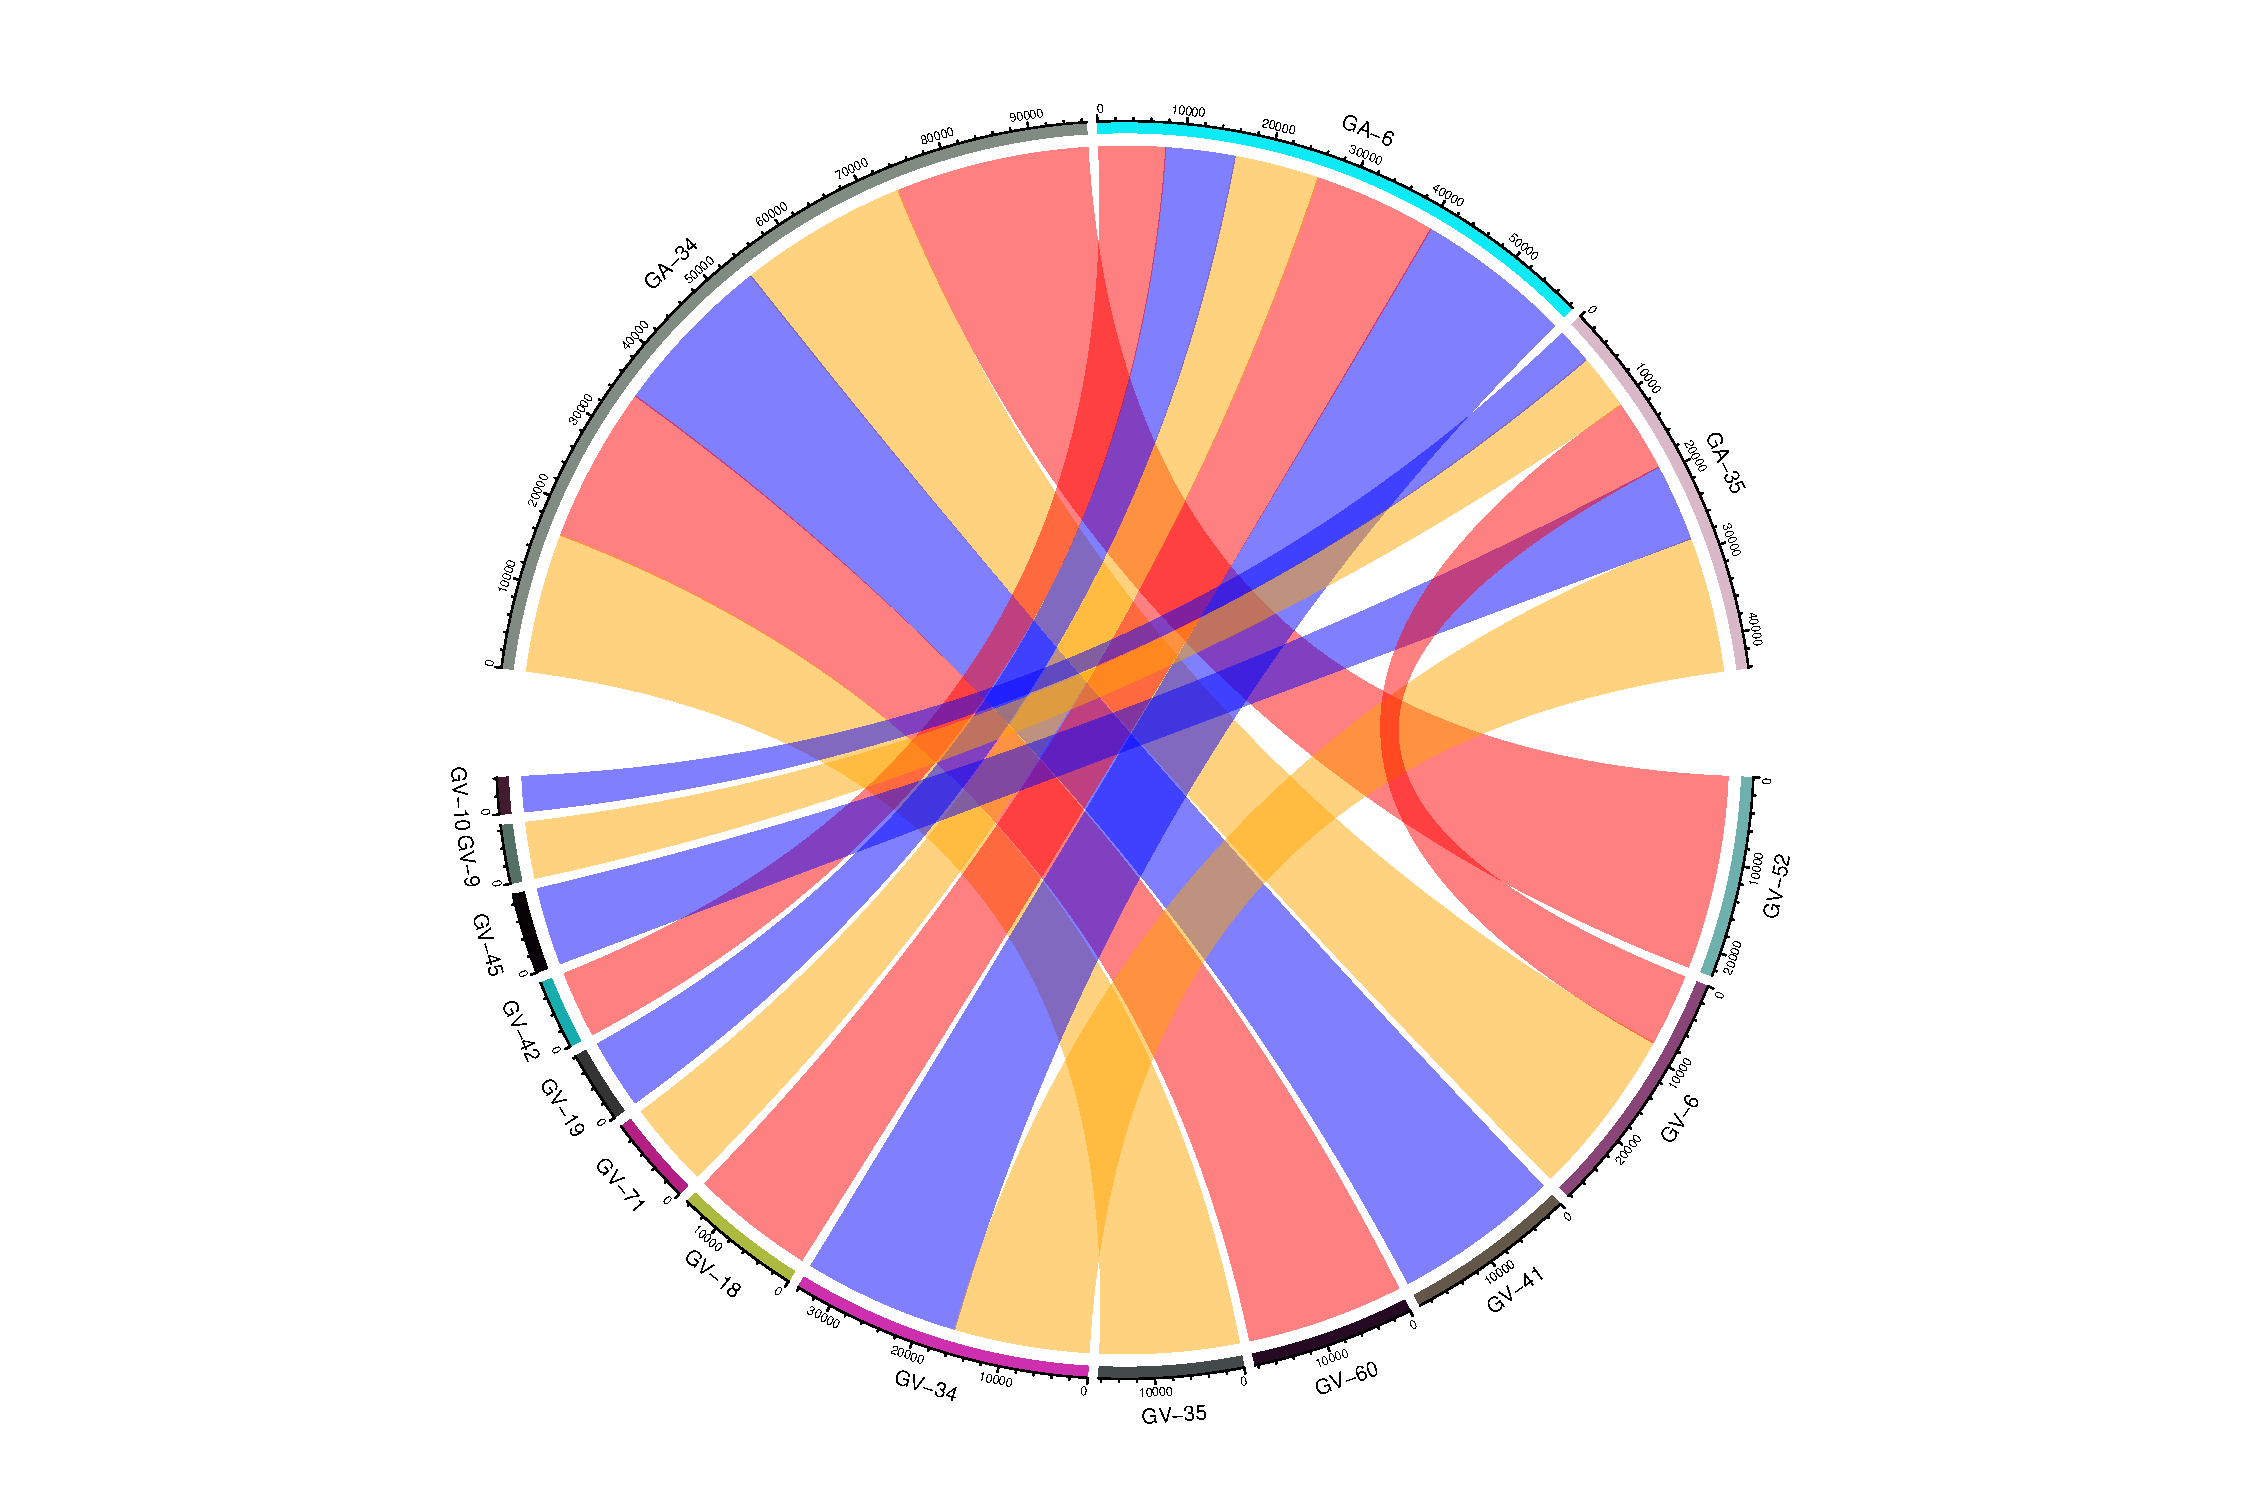
\includegraphics{rViz_files/figure-latex/unnamed-chunk-23-1.pdf}

\hypertarget{choropleth-map}{%
\section{Choropleth Map}\label{choropleth-map}}

\emph{İllere göre Covid-19 vaka sayısı (iller bazında ilk açıklandığı zamana ait veriler):}

\begin{Shaded}
\begin{Highlighting}[]
\NormalTok{TR <-}\StringTok{ }\KeywordTok{getData}\NormalTok{(}\StringTok{"GADM"}\NormalTok{, }\DataTypeTok{country =} \StringTok{"TR"}\NormalTok{, }\DataTypeTok{level =} \DecValTok{1}\NormalTok{) }\CommentTok{#Türkiye iller düzeyi}

\NormalTok{v8}\OperatorTok{$}\StringTok{`}\DataTypeTok{100KNüfus` <- round(v8$}\StringTok{`}\NormalTok{100KNüfus`, digits =}\StringTok{ }\DecValTok{0}\ErrorTok{)}

\NormalTok{palet <-}\StringTok{ }\KeywordTok{colorQuantile}\NormalTok{(}\DataTypeTok{palette =} \StringTok{"RdYlBu"}\NormalTok{, }\DataTypeTok{domain =}\NormalTok{ v8}\OperatorTok{$}\StringTok{`}\DataTypeTok{100KNüfus`, n = 5, reverse = TRUE) #Renk ayarları}

\DataTypeTok{leaflet() %>% }
\DataTypeTok{  addProviderTiles(providers$OpenStreetMap.Mapnik) %>% #Harita tipi}
\DataTypeTok{  addPolygons(data = TR,}
\DataTypeTok{              stroke = FALSE, smoothFactor = 0.2, fillOpacity = 0.3,}
\DataTypeTok{              fillColor = ~palet(v8$}\StringTok{`}\NormalTok{100KNüfus`),}
\NormalTok{              popup =}\StringTok{ }\KeywordTok{paste}\NormalTok{(}\StringTok{"<b>İl: </b>"}\NormalTok{, TR}\OperatorTok{$}\NormalTok{NAME_}\DecValTok{1}\NormalTok{, }\StringTok{"<br>"}\NormalTok{,}
                            \StringTok{"<b>Vaka Sayısı: </b>"}\NormalTok{, v8}\OperatorTok{$}\NormalTok{Vaka, }\StringTok{"<br>"}\NormalTok{,}
                            \StringTok{"<b>100 Bin Nüfus Başına: </b>"}\NormalTok{, v8}\OperatorTok{$}\StringTok{`}\DataTypeTok{100KNüfus`)) %>% #Bilgilendirme}
\DataTypeTok{  addLegend(position = "bottomright", pal = palet, values = v8$}\StringTok{`}\NormalTok{100KNüfus`, }\DataTypeTok{title =} \StringTok{""}\NormalTok{, }\DataTypeTok{opacity =} \DecValTok{1}\NormalTok{) }\CommentTok{#Lejant}
\end{Highlighting}
\end{Shaded}

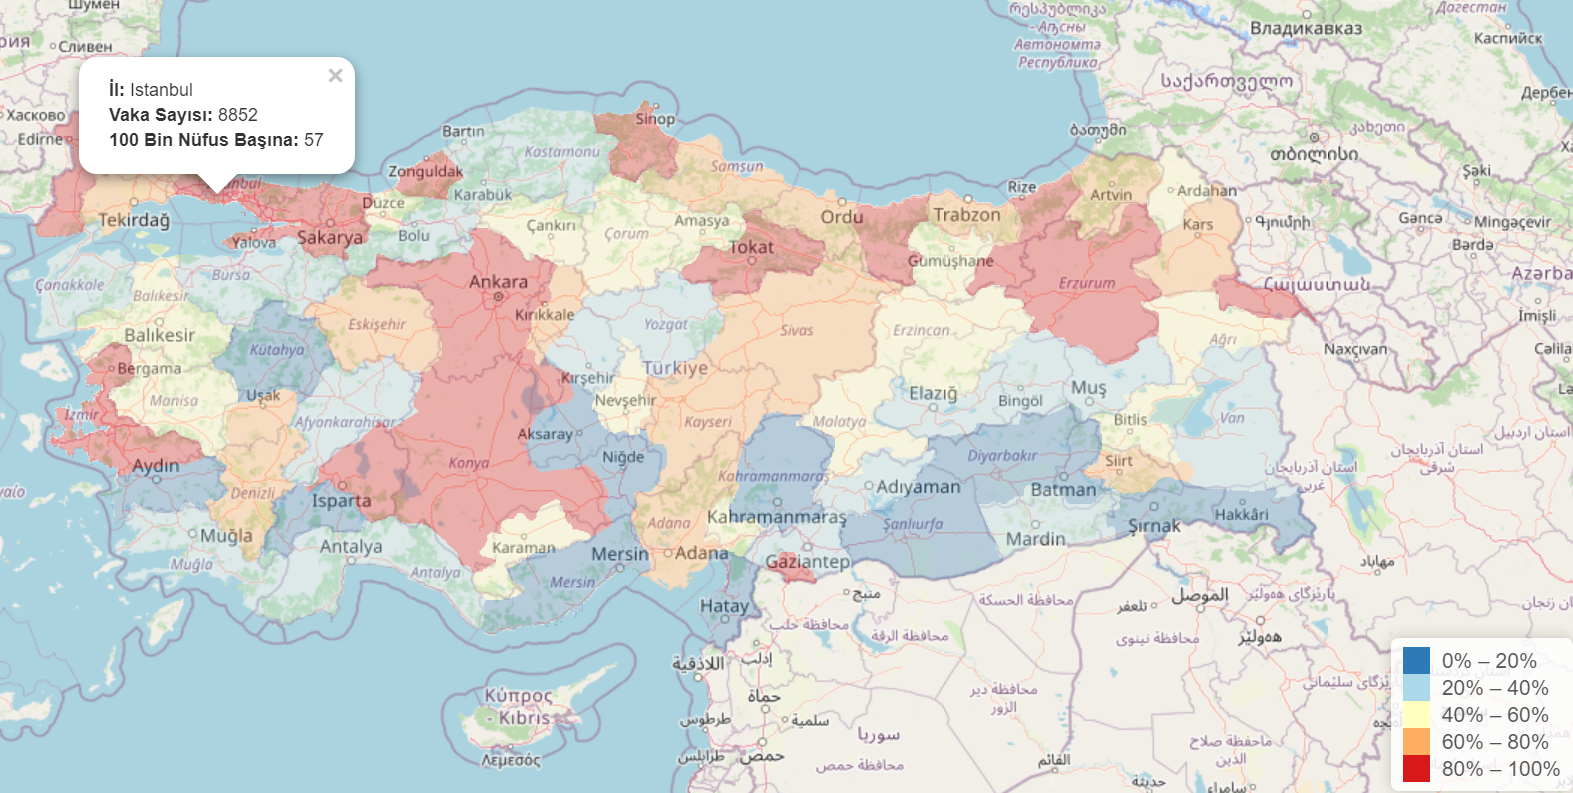
\includegraphics[width=1\linewidth]{C:/Users/datanerd/Desktop/Github/rViz/img/choropleth}

\hypertarget{circular}{%
\section{Circular}\label{circular}}

\emph{Ölümlü yaralanmalı trafik kazası sayısı:}

\begin{Shaded}
\begin{Highlighting}[]
\NormalTok{v28}\OperatorTok{$}\NormalTok{Ay <-}\StringTok{ }\KeywordTok{factor}\NormalTok{(}\DataTypeTok{x =}\NormalTok{ v28}\OperatorTok{$}\NormalTok{Ay, }\DataTypeTok{levels =} \KeywordTok{c}\NormalTok{(}\StringTok{"Ocak"}\NormalTok{,}\StringTok{"Şubat"}\NormalTok{,}\StringTok{"Mart"}\NormalTok{,}\StringTok{"Nisan"}\NormalTok{,}\StringTok{"Mayıs"}\NormalTok{,}\StringTok{"Haziran"}\NormalTok{,}
                                        \StringTok{"Temmuz"}\NormalTok{,}\StringTok{"Ağustos"}\NormalTok{,}\StringTok{"Eylül","}\NormalTok{Ekim}\StringTok{","}\NormalTok{Kasım}\StringTok{","}\NormalTok{Aralık}\StringTok{")) #Olması gereken sıralama}

\StringTok{#En basit şekilde}

\StringTok{ggplot(data = v28)+}
\StringTok{  geom_bar(aes(x = Ay, y = `Kaza Sayısı`), stat = "}\NormalTok{identity}\StringTok{") +}
\StringTok{  coord_polar()}
\end{Highlighting}
\end{Shaded}

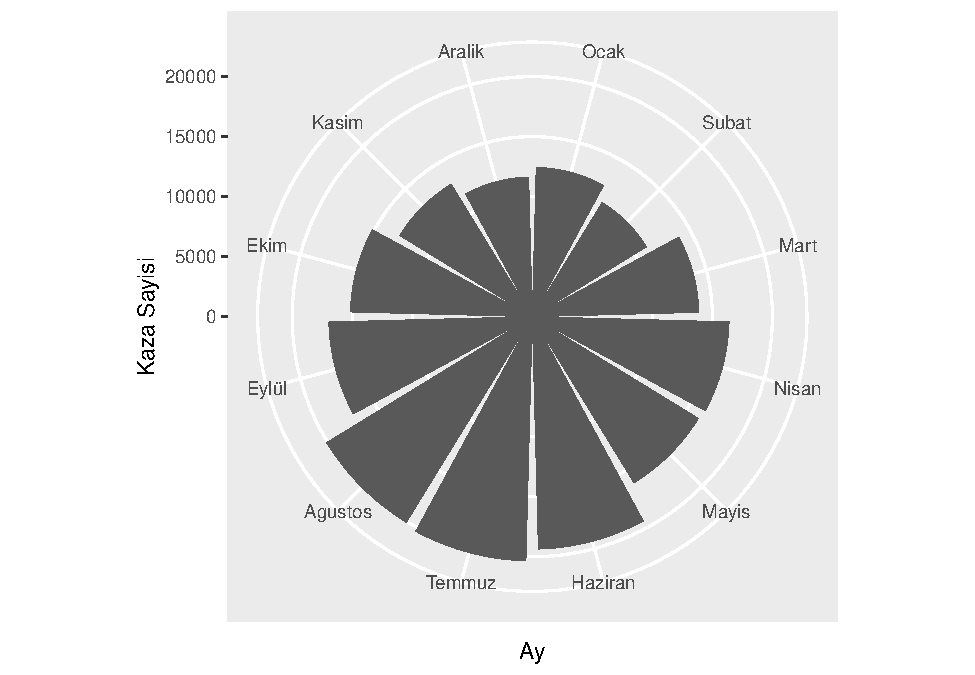
\includegraphics{rViz_files/figure-latex/unnamed-chunk-26-1.pdf}

\begin{itemize}
\item
  Renklendirebiliriz.
\item
  Genişliği ayarlayabiliriz.
\item
  y eksenine ait değerleri kaldırabiliriz.
\end{itemize}

\begin{Shaded}
\begin{Highlighting}[]
\KeywordTok{ggplot}\NormalTok{(}\DataTypeTok{data =}\NormalTok{ v28)}\OperatorTok{+}
\StringTok{  }\KeywordTok{geom_bar}\NormalTok{(}\KeywordTok{aes}\NormalTok{(}\DataTypeTok{x =}\NormalTok{ Ay, }\DataTypeTok{y =} \StringTok{`}\DataTypeTok{Kaza Sayısı}\StringTok{`}\NormalTok{, }\DataTypeTok{fill =}\NormalTok{ Ay), }\DataTypeTok{stat =} \StringTok{"identity"}\NormalTok{, }\DataTypeTok{width =} \FloatTok{0.9}\NormalTok{) }\OperatorTok{+}
\StringTok{  }\KeywordTok{coord_polar}\NormalTok{() }\OperatorTok{+}
\StringTok{  }\KeywordTok{scale_fill_viridis_d}\NormalTok{() }\OperatorTok{+}
\StringTok{  }\KeywordTok{theme}\NormalTok{(}\DataTypeTok{axis.text.y =} \KeywordTok{element_blank}\NormalTok{())}
\end{Highlighting}
\end{Shaded}

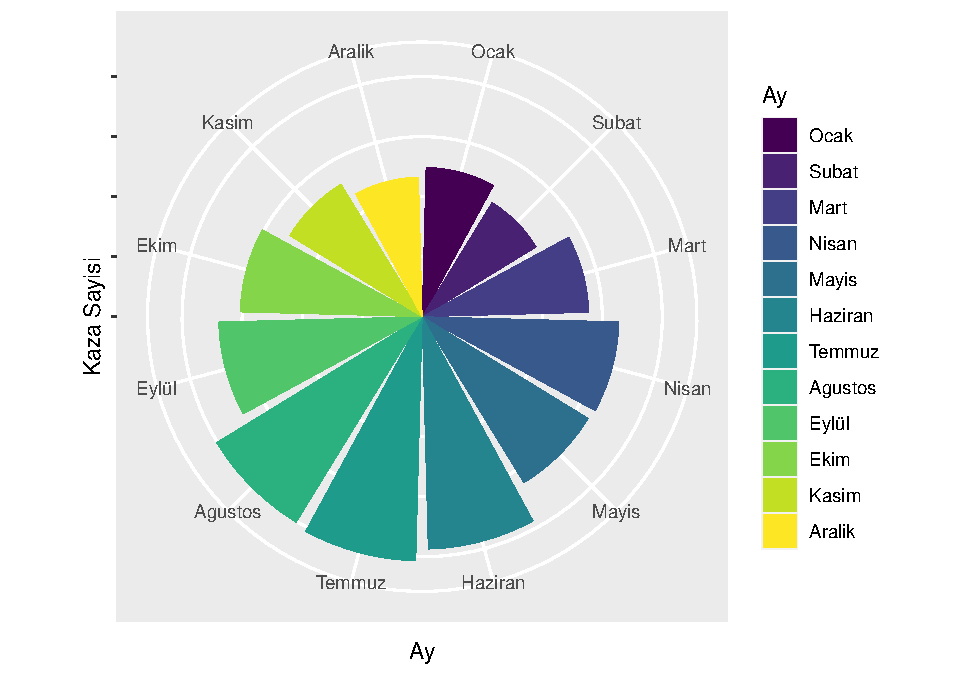
\includegraphics{rViz_files/figure-latex/unnamed-chunk-27-1.pdf}

\begin{itemize}
\item
  Lejantı kaldırabiliriz.
\item
  x ve y eksenlerine ait başlıkları kaldırabiliriz.
\item
  Başlık, alt başlık ve kaynak ekleyebiliriz.
\item
  Temayı değiştirebiliriz.
\end{itemize}

\begin{Shaded}
\begin{Highlighting}[]
\KeywordTok{ggplot}\NormalTok{(}\DataTypeTok{data =}\NormalTok{ v28)}\OperatorTok{+}
\StringTok{  }\KeywordTok{geom_bar}\NormalTok{(}\KeywordTok{aes}\NormalTok{(}\DataTypeTok{x =}\NormalTok{ Ay, }\DataTypeTok{y =} \StringTok{`}\DataTypeTok{Kaza Sayısı}\StringTok{`}\NormalTok{, }\DataTypeTok{fill =}\NormalTok{ Ay), }\DataTypeTok{stat =} \StringTok{"identity"}\NormalTok{, }\DataTypeTok{width =} \FloatTok{0.9}\NormalTok{) }\OperatorTok{+}
\StringTok{  }\KeywordTok{theme_minimal}\NormalTok{() }\OperatorTok{+}
\StringTok{  }\KeywordTok{scale_fill_viridis_d}\NormalTok{() }\OperatorTok{+}
\StringTok{  }\KeywordTok{coord_polar}\NormalTok{() }\OperatorTok{+}
\StringTok{  }\KeywordTok{theme}\NormalTok{(}\DataTypeTok{legend.position =} \StringTok{"none"}\NormalTok{,}
        \DataTypeTok{axis.title =} \KeywordTok{element_blank}\NormalTok{(),}
        \DataTypeTok{axis.text.y =} \KeywordTok{element_blank}\NormalTok{()) }\OperatorTok{+}
\StringTok{  }\KeywordTok{labs}\NormalTok{(}\DataTypeTok{x =} \OtherTok{NULL}\NormalTok{,}
       \DataTypeTok{y =} \OtherTok{NULL}\NormalTok{,}
       \DataTypeTok{title =} \StringTok{"Ölümlü Yaralanmalı Trafik Kazası Sayısı"}\NormalTok{,}
       \DataTypeTok{subtitle =} \StringTok{"2018 yılına ait verilerdir"}\NormalTok{,}
       \DataTypeTok{caption =} \StringTok{"Kaynak: TÜİK"}\NormalTok{)}
\end{Highlighting}
\end{Shaded}

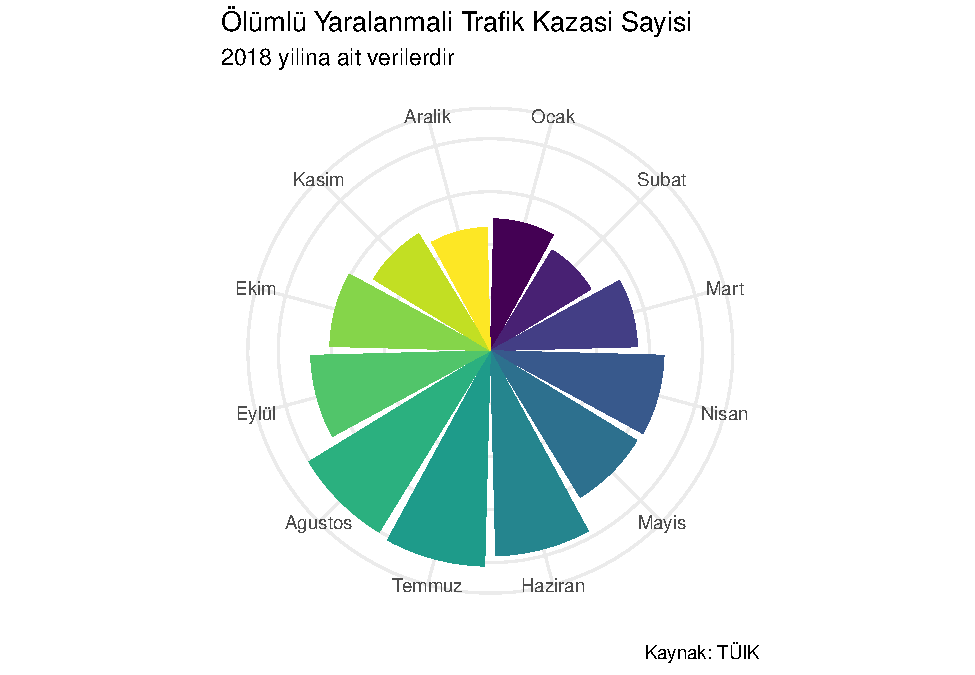
\includegraphics{rViz_files/figure-latex/unnamed-chunk-28-1.pdf}

\hypertarget{connected-scatter-baux11flantux131lux131-sauxe7ux131lux131m}{%
\section{Connected Scatter (Bağlantılı Saçılım)}\label{connected-scatter-baux11flantux131lux131-sauxe7ux131lux131m}}

\emph{TÜFE aylık değişim (\%):}

\begin{Shaded}
\begin{Highlighting}[]
\NormalTok{v10 }\OperatorTok\StringTok{ }
\StringTok{  }\KeywordTok{mutate}\NormalTok{(}\DataTypeTok{Tarih =} \KeywordTok{as.Date}\NormalTok{(}\KeywordTok{paste0}\NormalTok{(Tarih,}\StringTok{"-"}\NormalTok{,}\DecValTok{1}\NormalTok{)))}

\CommentTok{#En basit şekilde}

\KeywordTok{ggplot}\NormalTok{(}\DataTypeTok{data =}\NormalTok{ v10, }\DataTypeTok{mapping =} \KeywordTok{aes}\NormalTok{(}\DataTypeTok{x =}\NormalTok{ Tarih, }\DataTypeTok{y =} \StringTok{`}\DataTypeTok{Gerçek}\StringTok{`}\NormalTok{)) }\OperatorTok{+}
\StringTok{  }\KeywordTok{geom_point}\NormalTok{() }\OperatorTok{+}
\StringTok{  }\KeywordTok{geom_line}\NormalTok{()}
\end{Highlighting}
\end{Shaded}

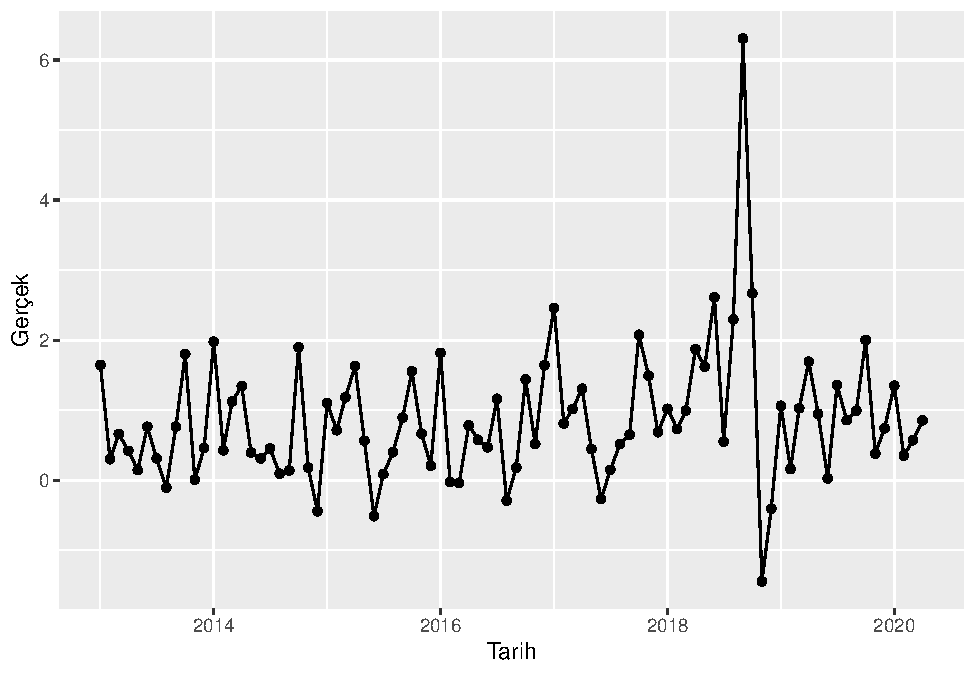
\includegraphics{rViz_files/figure-latex/unnamed-chunk-29-1.pdf}

\begin{itemize}
\item
  Mevsimlere göre renklendirebiliriz.
\item
  y ekseninde her bir yılı gösterebiliriz.
\item
  Çizgiyi daha soluk yapabiliriz.
\end{itemize}

\begin{Shaded}
\begin{Highlighting}[]
\KeywordTok{ggplot}\NormalTok{(}\DataTypeTok{data =}\NormalTok{ v10, }\DataTypeTok{mapping =} \KeywordTok{aes}\NormalTok{(}\DataTypeTok{x =}\NormalTok{ Tarih, }\DataTypeTok{y =} \StringTok{`}\DataTypeTok{Gerçek}\StringTok{`}\NormalTok{)) }\OperatorTok{+}
\StringTok{  }\KeywordTok{geom_point}\NormalTok{(}\KeywordTok{aes}\NormalTok{(}\DataTypeTok{color =}\NormalTok{ Mevsim)) }\OperatorTok{+}
\StringTok{  }\KeywordTok{geom_line}\NormalTok{(}\DataTypeTok{color =} \StringTok{"gray"}\NormalTok{) }\OperatorTok{+}
\StringTok{  }\KeywordTok{scale_x_date}\NormalTok{(}\DataTypeTok{date_breaks =} \StringTok{"year"}\NormalTok{, }\DataTypeTok{date_labels =} \StringTok{"%Y"}\NormalTok{)}
\end{Highlighting}
\end{Shaded}

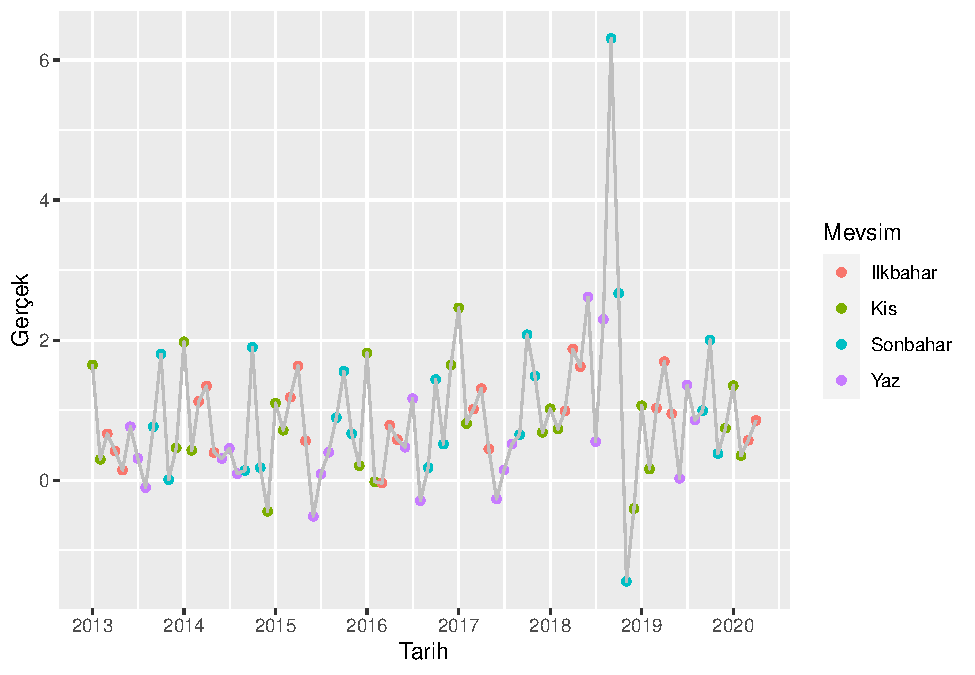
\includegraphics{rViz_files/figure-latex/unnamed-chunk-30-1.pdf}

\begin{itemize}
\item
  x eksenine ait başlığı kaldırabilir, y eksenine ait başlığı düzeltebiliriz.
\item
  Lejantı düzenleyebiliriz.
\item
  Başlık, alt başlık ve kaynak ekleyebiliriz.
\item
  Temayı değiştirebiliriz.
\end{itemize}

\begin{Shaded}
\begin{Highlighting}[]
\KeywordTok{ggplot}\NormalTok{(}\DataTypeTok{data =}\NormalTok{ v10, }\DataTypeTok{mapping =} \KeywordTok{aes}\NormalTok{(}\DataTypeTok{x =}\NormalTok{ Tarih, }\DataTypeTok{y =} \StringTok{`}\DataTypeTok{Gerçek}\StringTok{`}\NormalTok{)) }\OperatorTok{+}
\StringTok{  }\KeywordTok{geom_point}\NormalTok{(}\KeywordTok{aes}\NormalTok{(}\DataTypeTok{color =}\NormalTok{ Mevsim)) }\OperatorTok{+}
\StringTok{  }\KeywordTok{geom_line}\NormalTok{(}\DataTypeTok{color =} \StringTok{"gray"}\NormalTok{) }\OperatorTok{+}
\StringTok{  }\KeywordTok{theme_minimal}\NormalTok{() }\OperatorTok{+}
\StringTok{  }\KeywordTok{theme}\NormalTok{(}\DataTypeTok{legend.title =} \KeywordTok{element_blank}\NormalTok{()) }\OperatorTok{+}
\StringTok{  }\KeywordTok{scale_x_date}\NormalTok{(}\DataTypeTok{date_breaks =} \StringTok{"year"}\NormalTok{, }\DataTypeTok{date_labels =} \StringTok{"%Y"}\NormalTok{) }\OperatorTok{+}
\StringTok{  }\KeywordTok{labs}\NormalTok{(}\DataTypeTok{x =} \OtherTok{NULL}\NormalTok{,}
       \DataTypeTok{y =} \StringTok{"Değişim, %"}\NormalTok{,}
       \DataTypeTok{title =} \StringTok{"Aylık TÜFE Değişimi"}\NormalTok{,}
       \DataTypeTok{subtitle =} \StringTok{"2013/Ocak-2020/Nisan verilerine aittir"}\NormalTok{,}
       \DataTypeTok{caption =} \StringTok{"Kaynak: TÜİK"}\NormalTok{)}
\end{Highlighting}
\end{Shaded}

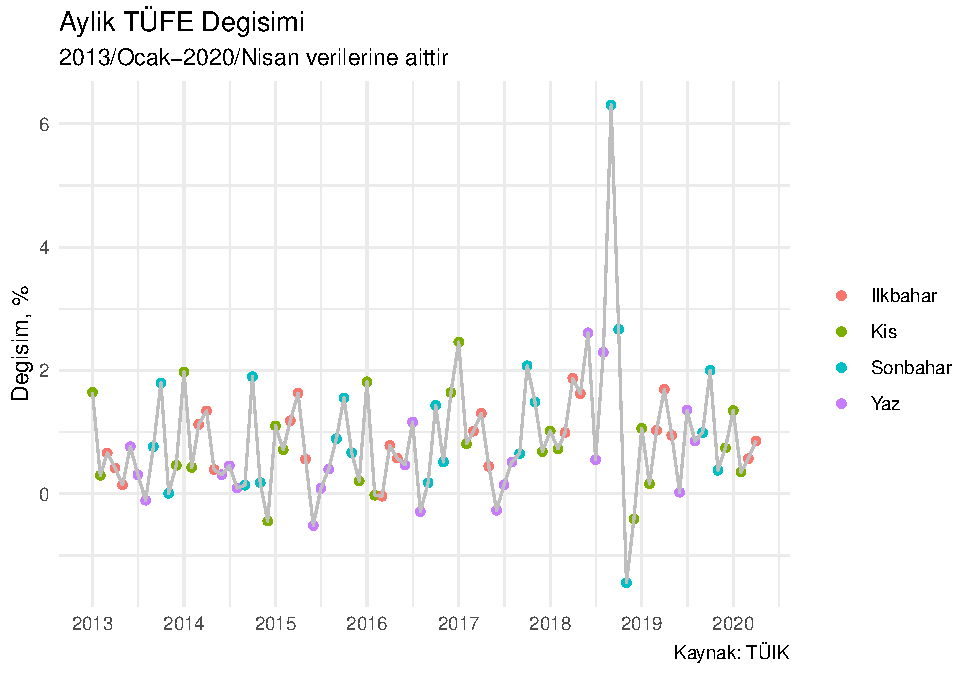
\includegraphics{rViz_files/figure-latex/unnamed-chunk-31-1.pdf}

\hypertarget{connection-map-baux11flantux131-harita}{%
\section{Connection Map (Bağlantı Harita)}\label{connection-map-baux11flantux131-harita}}

\emph{KTÜ'ye yerleşenlerin geldiği yerler (yokatlas):}

\begin{Shaded}
\begin{Highlighting}[]
\NormalTok{v11 }\OperatorTok\StringTok{ }
\StringTok{  }\KeywordTok{leaflet}\NormalTok{() }\OperatorTok
\StringTok{  }\KeywordTok{addTiles}\NormalTok{() }\OperatorTok
\StringTok{  }\KeywordTok{addPolylines}\NormalTok{(}\DataTypeTok{lng =} \OperatorTok{~}\NormalTok{long, }\DataTypeTok{lat =} \OperatorTok{~}\NormalTok{lat, }\DataTypeTok{weight =} \DecValTok{3}\NormalTok{, }\DataTypeTok{opacity =} \FloatTok{0.5}\NormalTok{) }\CommentTok{#Bağlantılar}
\end{Highlighting}
\end{Shaded}

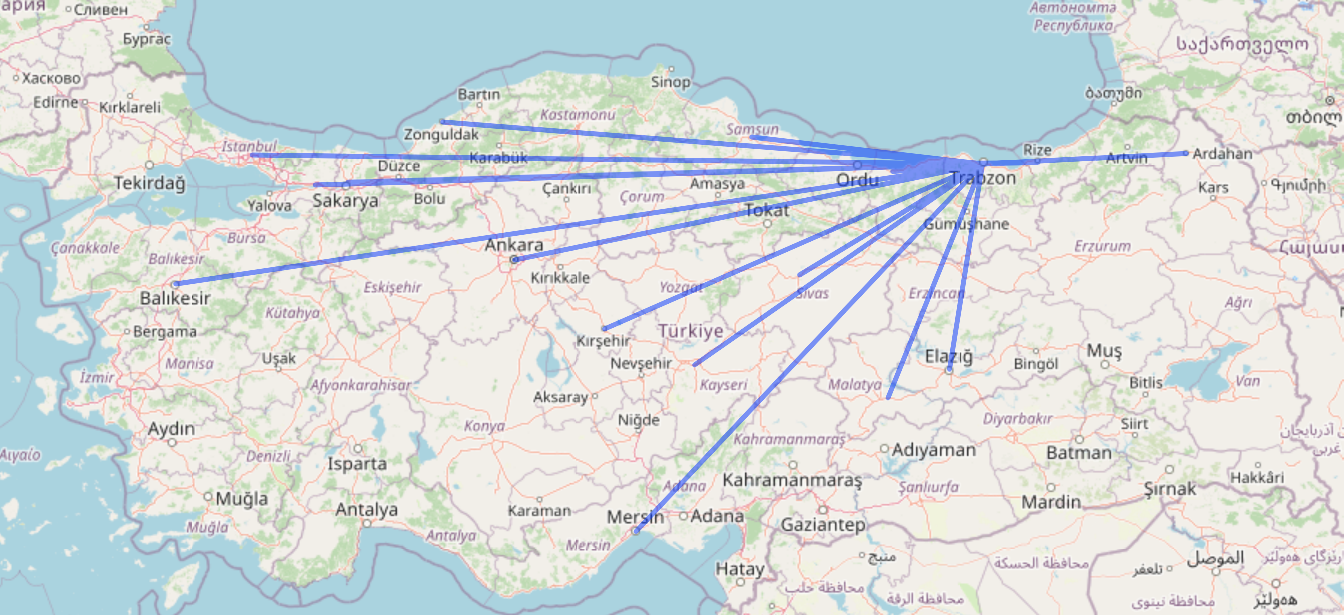
\includegraphics[width=1\linewidth]{C:/Users/datanerd/Desktop/Github/rViz/img/connection}

\hypertarget{density-youx11funluk}{%
\section{Density (Yoğunluk)}\label{density-youx11funluk}}

\emph{İstanbul Anadolu Yakası 1+1 kiralık daire fiyatları:}

\begin{Shaded}
\begin{Highlighting}[]
\CommentTok{#En basit şekilde}

\KeywordTok{ggplot}\NormalTok{(}\DataTypeTok{data =}\NormalTok{ v12, }\DataTypeTok{mapping =} \KeywordTok{aes}\NormalTok{(}\DataTypeTok{x =}\NormalTok{ Fiyat)) }\OperatorTok{+}
\StringTok{  }\KeywordTok{geom_density}\NormalTok{()}
\end{Highlighting}
\end{Shaded}

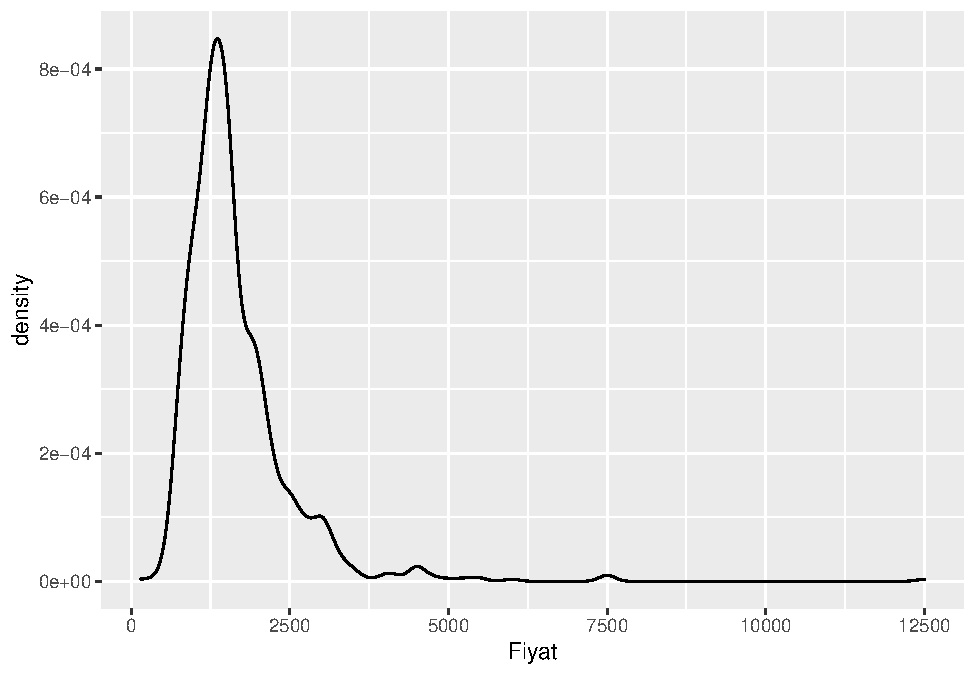
\includegraphics{rViz_files/figure-latex/unnamed-chunk-34-1.pdf}

\begin{itemize}
\item
  Renklendirme yapabiliriz.
\item
  y eksenine ait değerleri daha okunabilir bir formata getirebiliriz.
\end{itemize}

\begin{Shaded}
\begin{Highlighting}[]
\KeywordTok{ggplot}\NormalTok{(}\DataTypeTok{data =}\NormalTok{ v12, }\DataTypeTok{mapping =} \KeywordTok{aes}\NormalTok{(}\DataTypeTok{x =}\NormalTok{ Fiyat)) }\OperatorTok{+}
\StringTok{  }\KeywordTok{geom_density}\NormalTok{(}\DataTypeTok{fill =} \StringTok{"red"}\NormalTok{, }\DataTypeTok{color =} \StringTok{"red"}\NormalTok{, }\DataTypeTok{alpha =} \FloatTok{0.5}\NormalTok{) }\OperatorTok{+}
\StringTok{  }\KeywordTok{scale_y_continuous}\NormalTok{(}\DataTypeTok{labels =}\NormalTok{ comma)}
\end{Highlighting}
\end{Shaded}

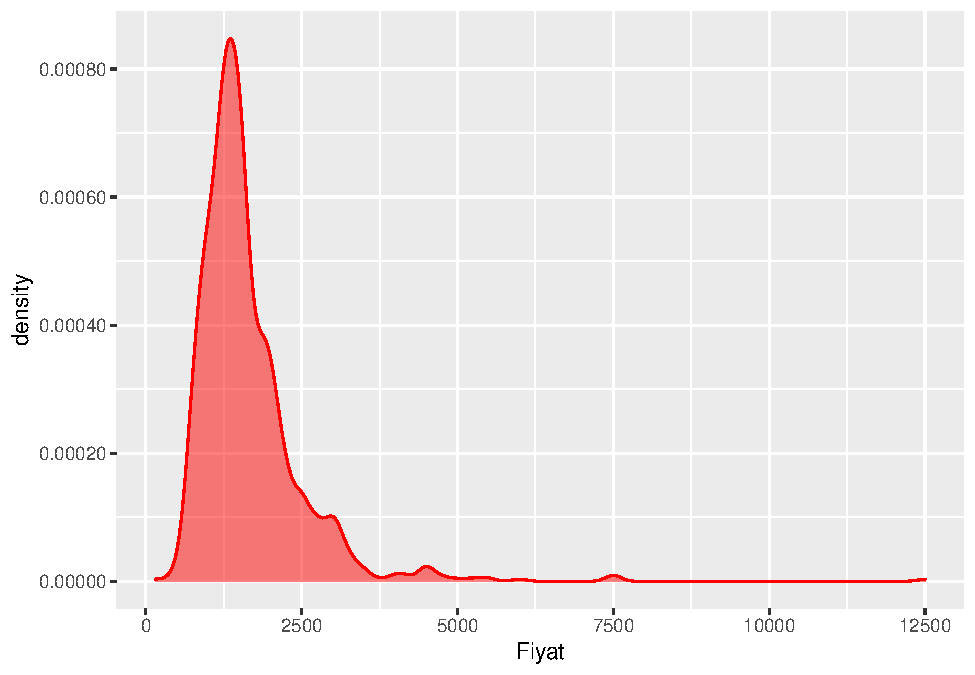
\includegraphics{rViz_files/figure-latex/unnamed-chunk-35-1.pdf}

\begin{itemize}
\item
  x eksenine ait başlığı kaldırabilir; y eksenine ait başlığı düzenleyebiliriz.
\item
  Başlık ve kaynak ekleyebiliriz.
\item
  Temayı değiştirebiliriz.
\end{itemize}

\begin{Shaded}
\begin{Highlighting}[]
\KeywordTok{ggplot}\NormalTok{(}\DataTypeTok{data =}\NormalTok{ v12, }\DataTypeTok{mapping =} \KeywordTok{aes}\NormalTok{(}\DataTypeTok{x =}\NormalTok{ Fiyat)) }\OperatorTok{+}
\StringTok{  }\KeywordTok{geom_density}\NormalTok{(}\DataTypeTok{fill =} \StringTok{"red"}\NormalTok{, }\DataTypeTok{color =} \StringTok{"red"}\NormalTok{, }\DataTypeTok{alpha =} \FloatTok{0.5}\NormalTok{) }\OperatorTok{+}
\StringTok{  }\KeywordTok{theme_minimal}\NormalTok{() }\OperatorTok{+}
\StringTok{  }\KeywordTok{scale_y_continuous}\NormalTok{(}\DataTypeTok{labels =}\NormalTok{ comma) }\OperatorTok{+}
\StringTok{  }\KeywordTok{labs}\NormalTok{(}\DataTypeTok{x =} \OtherTok{NULL}\NormalTok{,}
       \DataTypeTok{y =} \StringTok{"Yoğunluk"}\NormalTok{,}
       \DataTypeTok{title =} \StringTok{"İstanbul Anadolu Yakası'ndaki 1+1 Kiralık Daire Fiyatları"}\NormalTok{,}
       \DataTypeTok{caption =} \StringTok{"Kaynak: Sahibinden"}\NormalTok{)}
\end{Highlighting}
\end{Shaded}

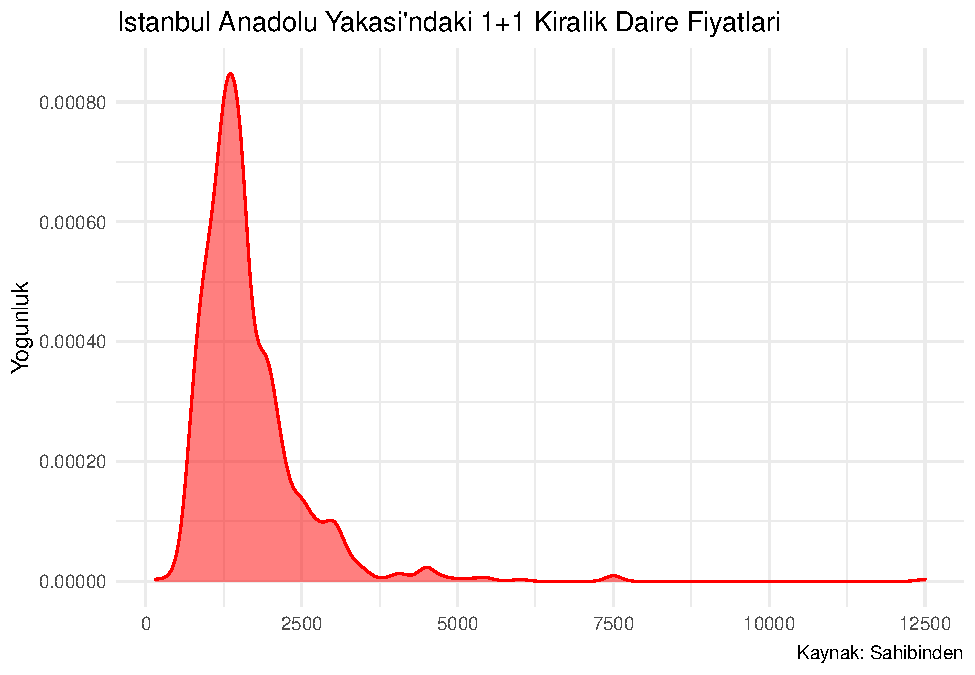
\includegraphics{rViz_files/figure-latex/unnamed-chunk-36-1.pdf}

\hypertarget{donut}{%
\section{Donut}\label{donut}}

\emph{23 Haziran 2019 İstanbul sonuçları:}

\begin{Shaded}
\begin{Highlighting}[]
\CommentTok{#En basit şekilde}

\NormalTok{v13}\OperatorTok{$}\NormalTok{Oran <-}\StringTok{ }\NormalTok{v13}\OperatorTok{$}\NormalTok{Oy }\OperatorTok{/}\StringTok{ }\KeywordTok{sum}\NormalTok{(v13}\OperatorTok{$}\NormalTok{Oy) }\CommentTok{#Oy oranları}
\NormalTok{v13}\OperatorTok{$}\NormalTok{ymax <-}\StringTok{ }\KeywordTok{cumsum}\NormalTok{(v13}\OperatorTok{$}\NormalTok{Oran) }\CommentTok{#Kümülatif oranlar}
\NormalTok{v13}\OperatorTok{$}\NormalTok{ymin =}\StringTok{ }\KeywordTok{c}\NormalTok{(}\DecValTok{0}\NormalTok{, }\KeywordTok{head}\NormalTok{(v13}\OperatorTok{$}\NormalTok{ymax, }\DataTypeTok{n =} \DecValTok{-1}\NormalTok{)) }\CommentTok{#Alan}

\KeywordTok{ggplot}\NormalTok{(v13, }\KeywordTok{aes}\NormalTok{(}\DataTypeTok{ymax =}\NormalTok{ ymax, }\DataTypeTok{ymin =}\NormalTok{ ymin, }\DataTypeTok{xmax =} \DecValTok{4}\NormalTok{, }\DataTypeTok{xmin =} \DecValTok{3}\NormalTok{, }\DataTypeTok{fill =}\NormalTok{ Aday)) }\OperatorTok{+}
\StringTok{  }\KeywordTok{geom_rect}\NormalTok{() }\OperatorTok{+}
\StringTok{  }\KeywordTok{coord_polar}\NormalTok{(}\DataTypeTok{theta =} \StringTok{"y"}\NormalTok{) }\OperatorTok{+}
\StringTok{  }\KeywordTok{xlim}\NormalTok{(}\KeywordTok{c}\NormalTok{(}\DecValTok{2}\NormalTok{, }\DecValTok{4}\NormalTok{))}
\end{Highlighting}
\end{Shaded}

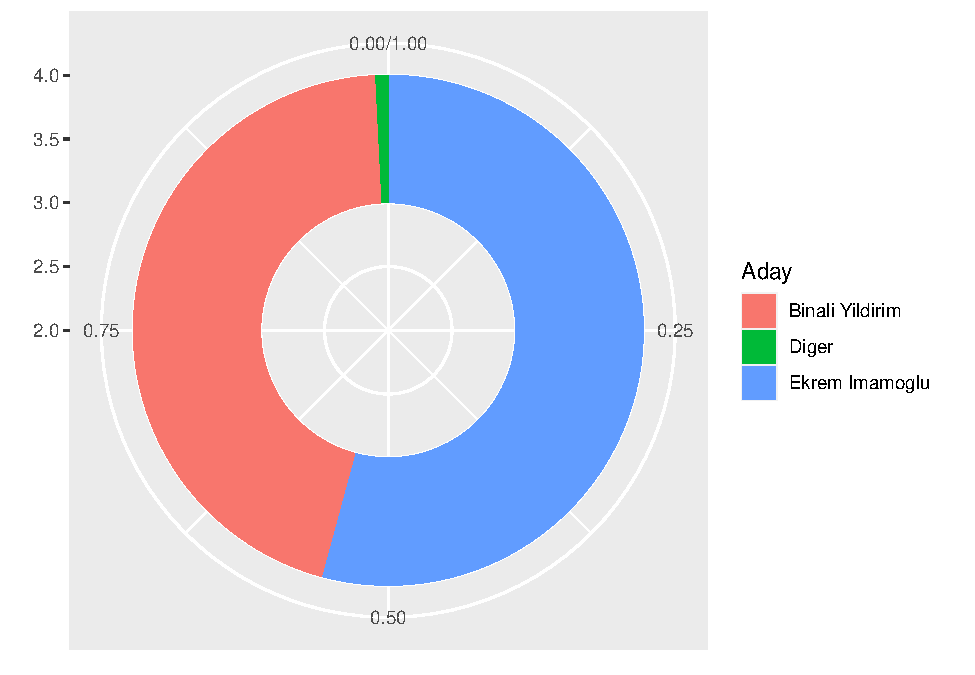
\includegraphics{rViz_files/figure-latex/unnamed-chunk-37-1.pdf}

\begin{itemize}
\item
  İsimlerin pozisyonlarını ayarlayabiliriz.
\item
  Etiketlerin gösterim şeklini ayarlayabiliriz.
\item
  Renklendirme yapabiliriz.
\end{itemize}

\begin{Shaded}
\begin{Highlighting}[]
\NormalTok{v13}\OperatorTok{$}\NormalTok{EtiketPoz <-}\StringTok{ }\NormalTok{(v13}\OperatorTok{$}\NormalTok{ymax }\OperatorTok{+}\StringTok{ }\NormalTok{v13}\OperatorTok{$}\NormalTok{ymin) }\OperatorTok{/}\StringTok{ }\DecValTok{2}
\NormalTok{v13}\OperatorTok{$}\NormalTok{Etiket <-}\StringTok{ }\KeywordTok{paste0}\NormalTok{(v13}\OperatorTok{$}\NormalTok{Aday, }\StringTok{"}\CharTok{\textbackslash{}n}\StringTok{%"}\NormalTok{, }\KeywordTok{round}\NormalTok{(v13}\OperatorTok{$}\NormalTok{Oran }\OperatorTok{*}\StringTok{ }\DecValTok{100}\NormalTok{, }\DataTypeTok{digits =} \DecValTok{2}\NormalTok{))}

\KeywordTok{ggplot}\NormalTok{(v13, }\KeywordTok{aes}\NormalTok{(}\DataTypeTok{ymax =}\NormalTok{ ymax, }\DataTypeTok{ymin =}\NormalTok{ ymin, }\DataTypeTok{xmax =} \DecValTok{4}\NormalTok{, }\DataTypeTok{xmin =} \DecValTok{3}\NormalTok{, }\DataTypeTok{fill =}\NormalTok{ Aday)) }\OperatorTok{+}
\StringTok{  }\KeywordTok{geom_rect}\NormalTok{() }\OperatorTok{+}
\StringTok{  }\KeywordTok{geom_text}\NormalTok{(}\DataTypeTok{x =} \FloatTok{3.5}\NormalTok{, }\KeywordTok{aes}\NormalTok{(}\DataTypeTok{y =}\NormalTok{ EtiketPoz, }\DataTypeTok{label =}\NormalTok{ Etiket), }\DataTypeTok{size =} \DecValTok{3}\NormalTok{) }\OperatorTok{+}
\StringTok{  }\KeywordTok{coord_polar}\NormalTok{(}\DataTypeTok{theta =} \StringTok{"y"}\NormalTok{) }\OperatorTok{+}
\StringTok{  }\KeywordTok{xlim}\NormalTok{(}\KeywordTok{c}\NormalTok{(}\DecValTok{2}\NormalTok{, }\DecValTok{4}\NormalTok{)) }\OperatorTok{+}
\StringTok{  }\KeywordTok{scale_fill_manual}\NormalTok{(}\DataTypeTok{values =} \KeywordTok{c}\NormalTok{(}\StringTok{"orange"}\NormalTok{, }\StringTok{"gray"}\NormalTok{, }\StringTok{"red"}\NormalTok{))}
\end{Highlighting}
\end{Shaded}

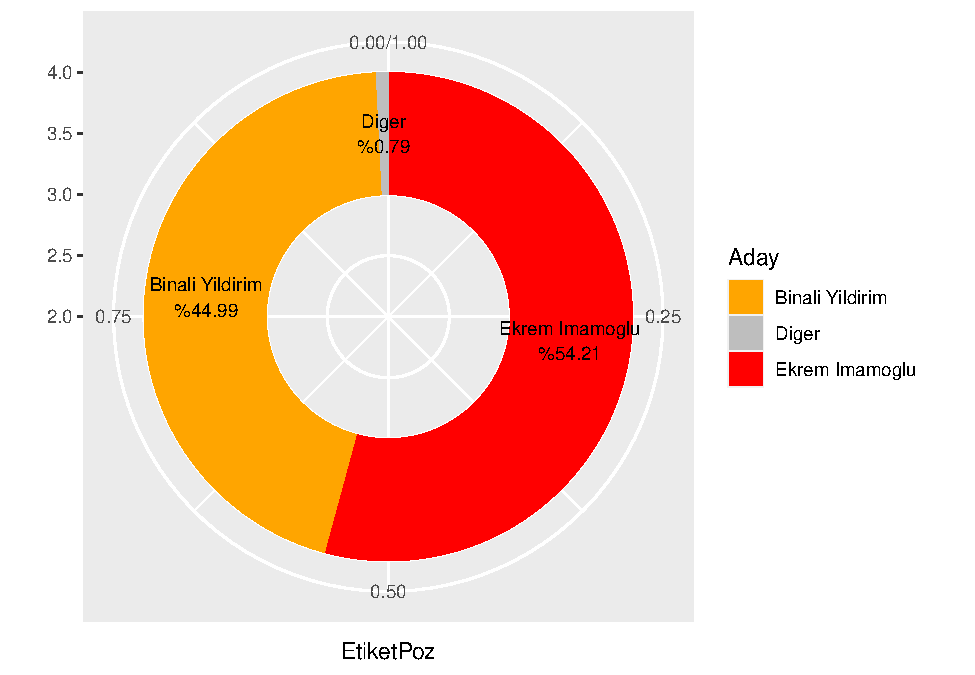
\includegraphics{rViz_files/figure-latex/unnamed-chunk-38-1.pdf}

\begin{itemize}
\item
  Lejantı kaldırabiliriz.
\item
  Başlık, alt başlık ve kaynak ekleyebiliriz.
\item
  Temayı değiştirebiliriz.
\end{itemize}

\begin{Shaded}
\begin{Highlighting}[]
\KeywordTok{ggplot}\NormalTok{(v13, }\KeywordTok{aes}\NormalTok{(}\DataTypeTok{ymax =}\NormalTok{ ymax, }\DataTypeTok{ymin =}\NormalTok{ ymin, }\DataTypeTok{xmax =} \DecValTok{4}\NormalTok{, }\DataTypeTok{xmin =} \DecValTok{3}\NormalTok{, }\DataTypeTok{fill =}\NormalTok{ Aday)) }\OperatorTok{+}
\StringTok{  }\KeywordTok{geom_rect}\NormalTok{() }\OperatorTok{+}
\StringTok{  }\KeywordTok{geom_text}\NormalTok{(}\DataTypeTok{x =} \FloatTok{3.5}\NormalTok{, }\KeywordTok{aes}\NormalTok{(}\DataTypeTok{y =}\NormalTok{ EtiketPoz, }\DataTypeTok{label =}\NormalTok{ Etiket), }\DataTypeTok{size =} \DecValTok{3}\NormalTok{) }\OperatorTok{+}
\StringTok{  }\KeywordTok{theme_void}\NormalTok{() }\OperatorTok{+}
\StringTok{  }\KeywordTok{coord_polar}\NormalTok{(}\DataTypeTok{theta =} \StringTok{"y"}\NormalTok{) }\OperatorTok{+}
\StringTok{  }\KeywordTok{xlim}\NormalTok{(}\KeywordTok{c}\NormalTok{(}\DecValTok{2}\NormalTok{, }\DecValTok{4}\NormalTok{)) }\OperatorTok{+}
\StringTok{  }\KeywordTok{scale_fill_manual}\NormalTok{(}\DataTypeTok{values =} \KeywordTok{c}\NormalTok{(}\StringTok{"orange"}\NormalTok{, }\StringTok{"gray"}\NormalTok{, }\StringTok{"red"}\NormalTok{)) }\OperatorTok{+}
\StringTok{  }\KeywordTok{theme}\NormalTok{(}\DataTypeTok{legend.position =} \StringTok{"none"}\NormalTok{) }\OperatorTok{+}
\StringTok{  }\KeywordTok{labs}\NormalTok{(}\DataTypeTok{title =} \StringTok{"İstanbul Seçim Sonuçları"}\NormalTok{,}
       \DataTypeTok{subtitle =} \StringTok{"23 Haziran 2019"}\NormalTok{,}
       \DataTypeTok{caption =} \StringTok{"Kaynak: NTV"}\NormalTok{)}
\end{Highlighting}
\end{Shaded}

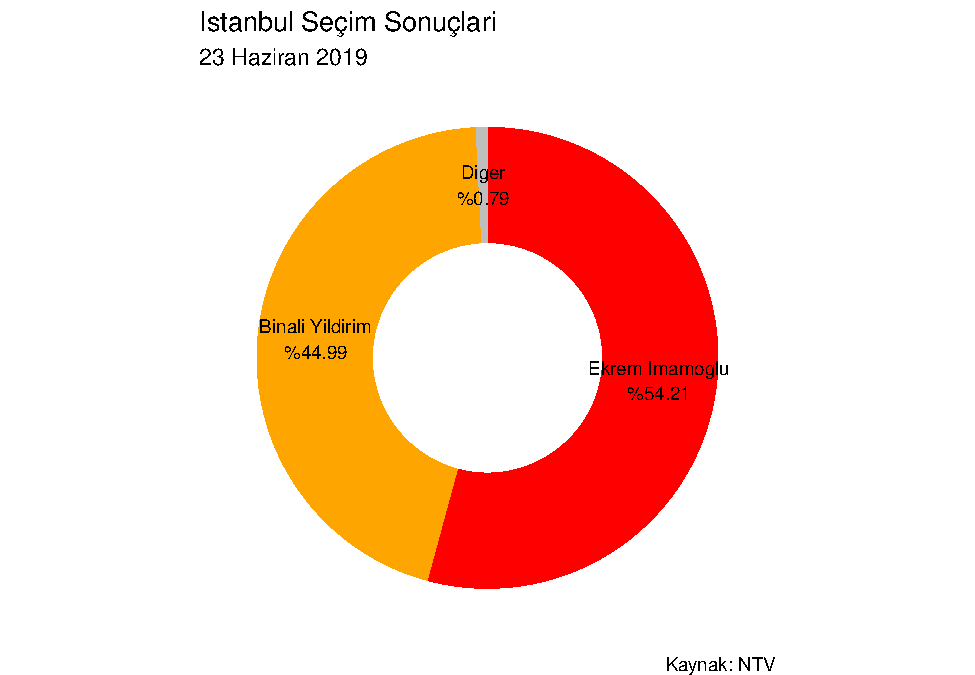
\includegraphics{rViz_files/figure-latex/unnamed-chunk-39-1.pdf}

\hypertarget{dot-map-nokta-haritasux131}{%
\section{Dot Map (Nokta Haritası)}\label{dot-map-nokta-haritasux131}}

\emph{Tiplerine göre Türkiye'deki havaalanları (wikipedia):}

\begin{Shaded}
\begin{Highlighting}[]
\NormalTok{palet <-}\StringTok{ }\KeywordTok{colorFactor}\NormalTok{(}\DataTypeTok{palette =} \KeywordTok{c}\NormalTok{(}\StringTok{"red"}\NormalTok{,}\StringTok{"gray"}\NormalTok{,}\StringTok{"orange"}\NormalTok{,}\StringTok{"blue"}\NormalTok{), }\DataTypeTok{domain =}\NormalTok{ v14}\OperatorTok{$}\NormalTok{Tip)}

\NormalTok{v14 }\OperatorTok\StringTok{ }
\StringTok{  }\KeywordTok{leaflet}\NormalTok{() }\OperatorTok\StringTok{ }
\StringTok{  }\KeywordTok{addTiles}\NormalTok{() }\OperatorTok
\StringTok{  }\KeywordTok{addProviderTiles}\NormalTok{(}\DataTypeTok{provider =}\NormalTok{ providers}\OperatorTok{$}\NormalTok{CartoDB.DarkMatterNoLabels) }\OperatorTok\StringTok{ }\CommentTok{#Harita tipi}
\StringTok{  }\KeywordTok{addCircles}\NormalTok{(}\DataTypeTok{lng =} \OperatorTok{~}\NormalTok{Koord2, }\DataTypeTok{lat =} \OperatorTok{~}\NormalTok{Koord1, }\DataTypeTok{weight =} \DecValTok{3}\NormalTok{, }\DataTypeTok{color =} \OperatorTok{~}\KeywordTok{palet}\NormalTok{(Tip)) }\OperatorTok\StringTok{ }\CommentTok{#Nokta}
\StringTok{  }\KeywordTok{addLegend}\NormalTok{(}\DataTypeTok{position =} \StringTok{"bottomright"}\NormalTok{, }\DataTypeTok{pal =}\NormalTok{ palet, }\DataTypeTok{values =}\NormalTok{ v14}\OperatorTok{$}\NormalTok{Tip, }\DataTypeTok{title =} \StringTok{""}\NormalTok{, }\DataTypeTok{opacity =} \DecValTok{1}\NormalTok{) }\CommentTok{#Lejant}
\end{Highlighting}
\end{Shaded}

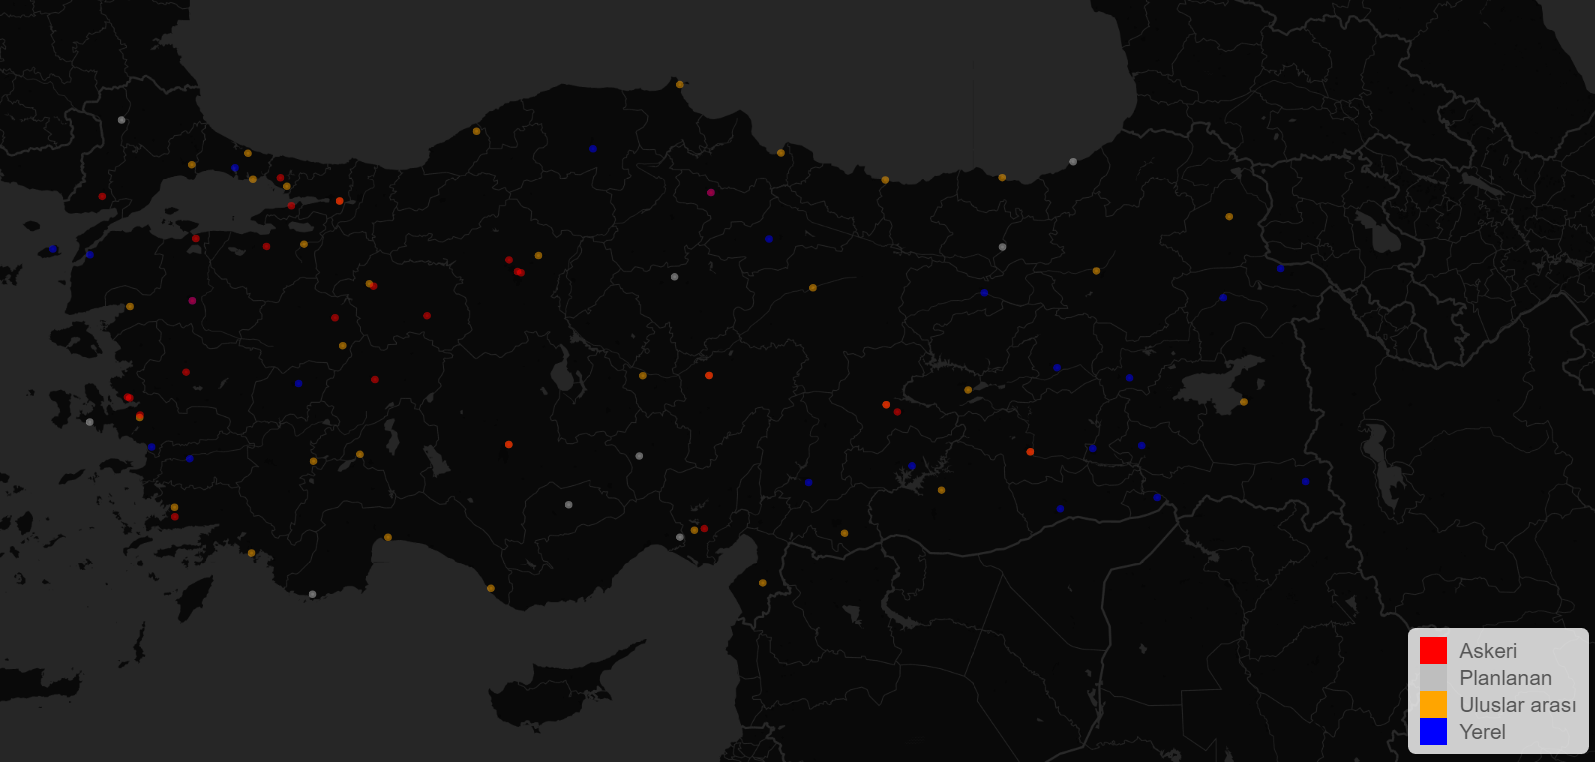
\includegraphics[width=1\linewidth]{C:/Users/datanerd/Desktop/Github/rViz/img/dot}

\hypertarget{dumbbell}{%
\section{Dumbbell}\label{dumbbell}}

\emph{Bölgelere ve cinsiyetlere göre ortalama ilk evlenme yaşları:}

\begin{Shaded}
\begin{Highlighting}[]
\CommentTok{#En basit şekilde}

\KeywordTok{ggplot}\NormalTok{(}\DataTypeTok{data =}\NormalTok{ v15)}\OperatorTok{+}
\StringTok{  }\KeywordTok{geom_dumbbell}\NormalTok{(}\DataTypeTok{mapping =} \KeywordTok{aes}\NormalTok{(}\DataTypeTok{x =} \StringTok{`}\DataTypeTok{Kadın}\StringTok{`}\NormalTok{, }\DataTypeTok{xend =}\NormalTok{ Erkek, }\DataTypeTok{y =} \StringTok{`}\DataTypeTok{Bölge}\StringTok{`}\NormalTok{))}
\end{Highlighting}
\end{Shaded}

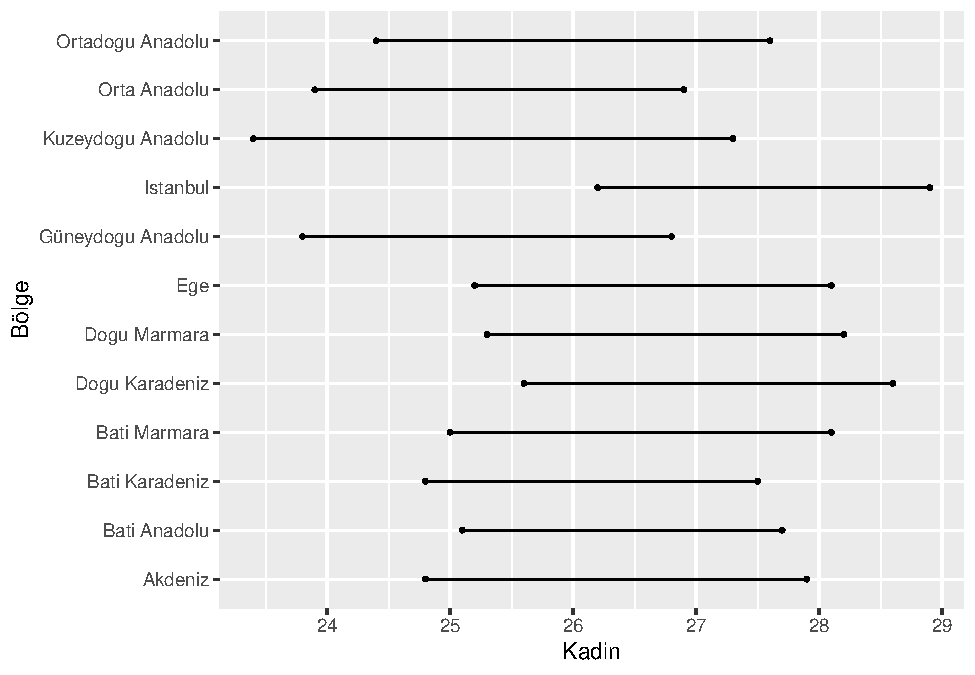
\includegraphics{rViz_files/figure-latex/unnamed-chunk-42-1.pdf}

\begin{itemize}
\item
  x ve xend büyüklüklerini ve renklerini belirleyebiliriz.
\item
  İki nokta arasındaki çizginin görünürlüğünü azaltabiliriz.
\end{itemize}

\begin{Shaded}
\begin{Highlighting}[]
\KeywordTok{ggplot}\NormalTok{(}\DataTypeTok{data =}\NormalTok{ v15)}\OperatorTok{+}
\StringTok{  }\KeywordTok{geom_dumbbell}\NormalTok{(}\DataTypeTok{mapping =} \KeywordTok{aes}\NormalTok{(}\DataTypeTok{x =} \StringTok{`}\DataTypeTok{Kadın}\StringTok{`}\NormalTok{, }\DataTypeTok{xend =}\NormalTok{ Erkek, }\DataTypeTok{y =} \StringTok{`}\DataTypeTok{Bölge}\StringTok{`}\NormalTok{),}
                \DataTypeTok{size_x =} \DecValTok{2}\NormalTok{, }\DataTypeTok{size_xend =} \DecValTok{2}\NormalTok{,}
                \DataTypeTok{colour_x =} \StringTok{"blue"}\NormalTok{, }\DataTypeTok{colour_xend =} \StringTok{"red"}\NormalTok{,}
                \DataTypeTok{colour =} \StringTok{"grey"}\NormalTok{)}
\end{Highlighting}
\end{Shaded}

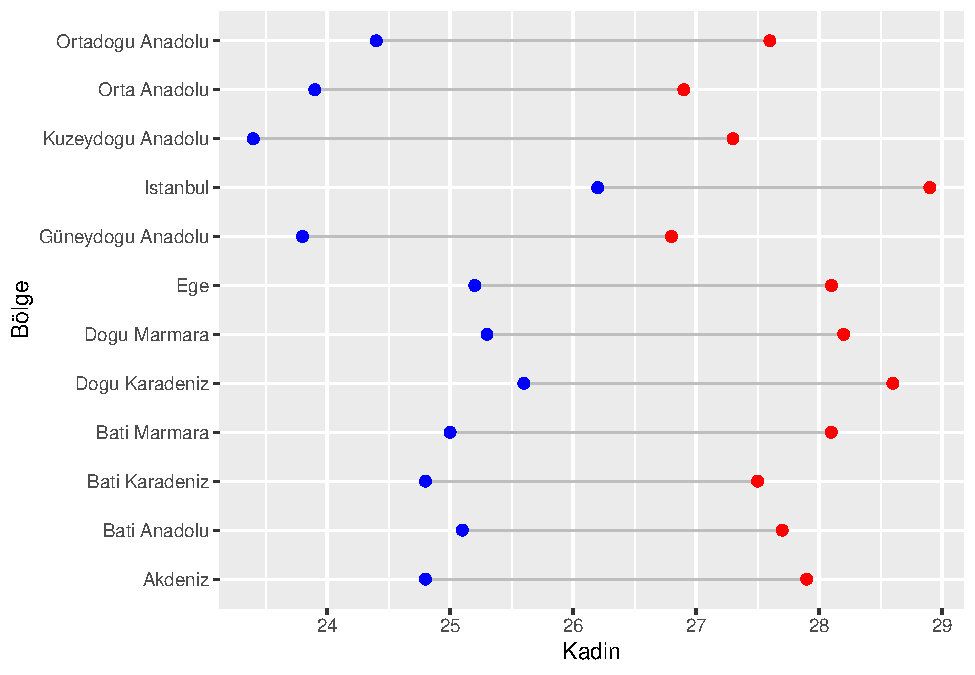
\includegraphics{rViz_files/figure-latex/unnamed-chunk-43-1.pdf}

\begin{itemize}
\item
  x eksenine ait limit ve aralıkları belirleyebiliriz.
\item
  x ve y eksenlerine ait başlıkları kaldırabiliriz.
\item
  Başlık, alt başlık ve kaynak ekleyebiliriz.
\item
  Temayı değiştirebiliriz.
\end{itemize}

\begin{Shaded}
\begin{Highlighting}[]
\KeywordTok{ggplot}\NormalTok{(}\DataTypeTok{data =}\NormalTok{ v15)}\OperatorTok{+}
\StringTok{  }\KeywordTok{geom_dumbbell}\NormalTok{(}\DataTypeTok{mapping =} \KeywordTok{aes}\NormalTok{(}\DataTypeTok{x =} \StringTok{`}\DataTypeTok{Kadın}\StringTok{`}\NormalTok{, }\DataTypeTok{xend =}\NormalTok{ Erkek, }\DataTypeTok{y =} \StringTok{`}\DataTypeTok{Bölge}\StringTok{`}\NormalTok{),}
                \DataTypeTok{size_x =} \DecValTok{2}\NormalTok{, }\DataTypeTok{size_xend =} \DecValTok{2}\NormalTok{,}
                \DataTypeTok{colour_x =} \StringTok{"blue"}\NormalTok{, }\DataTypeTok{colour_xend =} \StringTok{"red"}\NormalTok{,}
                \DataTypeTok{colour =} \StringTok{"grey"}\NormalTok{) }\OperatorTok{+}
\StringTok{  }\KeywordTok{theme_minimal}\NormalTok{() }\OperatorTok{+}
\StringTok{  }\KeywordTok{scale_x_continuous}\NormalTok{(}\DataTypeTok{limits =} \KeywordTok{c}\NormalTok{(}\DecValTok{23}\NormalTok{,}\DecValTok{30}\NormalTok{), }\DataTypeTok{breaks =} \KeywordTok{seq}\NormalTok{(}\DecValTok{23}\NormalTok{,}\DecValTok{30}\NormalTok{,}\DecValTok{1}\NormalTok{)) }\OperatorTok{+}
\StringTok{  }\KeywordTok{labs}\NormalTok{(}\DataTypeTok{x =} \OtherTok{NULL}\NormalTok{,}
       \DataTypeTok{y =} \OtherTok{NULL}\NormalTok{,}
       \DataTypeTok{title =} \StringTok{"Bölgelere ve Cinsiyetlere Göre Ortalama İlk Evlenme Yaşları"}\NormalTok{,}
       \DataTypeTok{subtitle =} \StringTok{"2019 yılına ait verilerdir"}\NormalTok{,}
       \DataTypeTok{caption =} \StringTok{"Kaynak: TÜİK"}\NormalTok{)}
\end{Highlighting}
\end{Shaded}

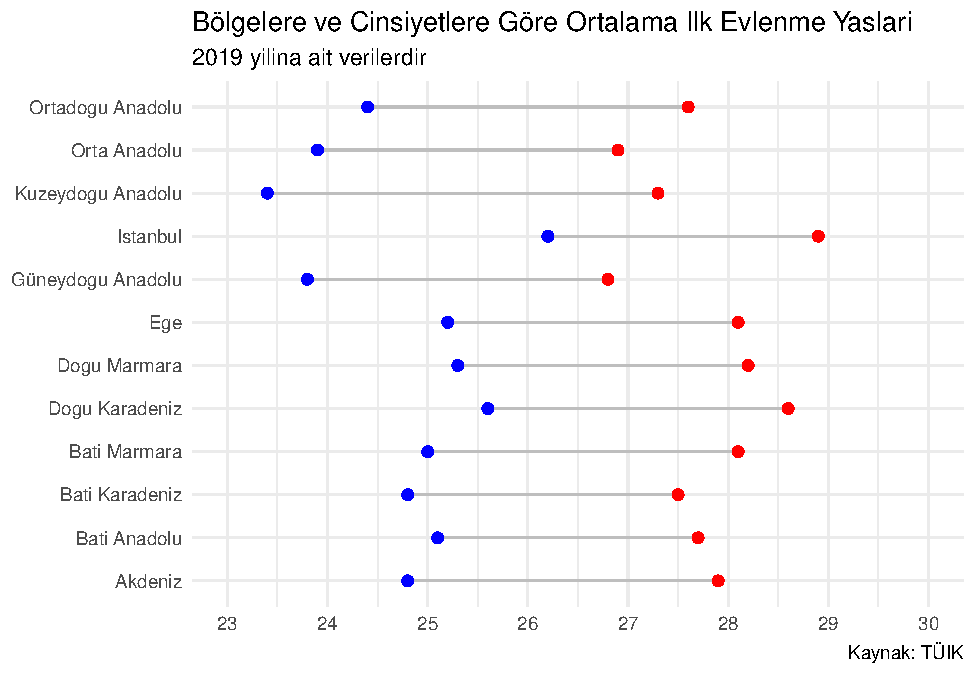
\includegraphics{rViz_files/figure-latex/unnamed-chunk-44-1.pdf}

\begin{itemize}
\tightlist
\item
  Noktaların hangi cinsiyete ait olduğunu da belirtebiliriz. Bunu yaparken her bir bölgeye ait çizgide de gösterebiliriz; aşağıda olduğu gibi bir tane bölgeyi filtreleyip tek bir çizgide de gösterebiliriz.
\end{itemize}

\begin{Shaded}
\begin{Highlighting}[]
\KeywordTok{ggplot}\NormalTok{(}\DataTypeTok{data =}\NormalTok{ v15)}\OperatorTok{+}
\StringTok{  }\KeywordTok{geom_dumbbell}\NormalTok{(}\DataTypeTok{mapping =} \KeywordTok{aes}\NormalTok{(}\DataTypeTok{x =} \StringTok{`}\DataTypeTok{Kadın}\StringTok{`}\NormalTok{, }\DataTypeTok{xend =}\NormalTok{ Erkek, }\DataTypeTok{y =} \StringTok{`}\DataTypeTok{Bölge}\StringTok{`}\NormalTok{),}
                \DataTypeTok{size_x =} \DecValTok{2}\NormalTok{, }\DataTypeTok{size_xend =} \DecValTok{2}\NormalTok{,}
                \DataTypeTok{colour_x =} \StringTok{"blue"}\NormalTok{, }\DataTypeTok{colour_xend =} \StringTok{"red"}\NormalTok{,}
                \DataTypeTok{colour =} \StringTok{"grey"}\NormalTok{) }\OperatorTok{+}
\StringTok{  }\KeywordTok{geom_text}\NormalTok{(}\DataTypeTok{data =}\NormalTok{ v15 }\OperatorTok\StringTok{ }\KeywordTok{filter}\NormalTok{(}\StringTok{`}\DataTypeTok{Bölge}\StringTok{`} \OperatorTok{==}\StringTok{ "Ortadoğu Anadolu"}\NormalTok{),}
            \KeywordTok{aes}\NormalTok{(}\DataTypeTok{x =} \StringTok{`}\DataTypeTok{Kadın}\StringTok{`}\NormalTok{, }\DataTypeTok{y =} \StringTok{`}\DataTypeTok{Bölge}\StringTok{`}\NormalTok{, }\DataTypeTok{label =} \StringTok{"Kadın"}\NormalTok{), }\DataTypeTok{size =} \DecValTok{3}\NormalTok{, }\DataTypeTok{hjust =} \FloatTok{1.2}\NormalTok{) }\OperatorTok{+}
\StringTok{  }\KeywordTok{geom_text}\NormalTok{(}\DataTypeTok{data =}\NormalTok{ v15 }\OperatorTok\StringTok{ }\KeywordTok{filter}\NormalTok{(}\StringTok{`}\DataTypeTok{Bölge}\StringTok{`} \OperatorTok{==}\StringTok{ "Ortadoğu Anadolu"}\NormalTok{),}
            \KeywordTok{aes}\NormalTok{(}\DataTypeTok{x =} \StringTok{`}\DataTypeTok{Erkek}\StringTok{`}\NormalTok{, }\DataTypeTok{y =} \StringTok{`}\DataTypeTok{Bölge}\StringTok{`}\NormalTok{, }\DataTypeTok{label =} \StringTok{"Erkek"}\NormalTok{), }\DataTypeTok{size =} \DecValTok{3}\NormalTok{, }\DataTypeTok{hjust =} \FloatTok{-0.2}\NormalTok{) }\OperatorTok{+}
\StringTok{  }\KeywordTok{theme_minimal}\NormalTok{() }\OperatorTok{+}
\StringTok{  }\KeywordTok{scale_x_continuous}\NormalTok{(}\DataTypeTok{limits =} \KeywordTok{c}\NormalTok{(}\DecValTok{23}\NormalTok{,}\DecValTok{30}\NormalTok{), }\DataTypeTok{breaks =} \KeywordTok{seq}\NormalTok{(}\DecValTok{23}\NormalTok{,}\DecValTok{30}\NormalTok{,}\DecValTok{1}\NormalTok{)) }\OperatorTok{+}
\StringTok{  }\KeywordTok{labs}\NormalTok{(}\DataTypeTok{x =} \OtherTok{NULL}\NormalTok{,}
       \DataTypeTok{y =} \OtherTok{NULL}\NormalTok{,}
       \DataTypeTok{title =} \StringTok{"Bölgelere ve Cinsiyetlere Göre Ortalama İlk Evlenme Yaşları"}\NormalTok{,}
       \DataTypeTok{subtitle =} \StringTok{"2019 yılına ait verilerdir"}\NormalTok{,}
       \DataTypeTok{caption =} \StringTok{"Kaynak: TÜİK"}\NormalTok{)}
\end{Highlighting}
\end{Shaded}

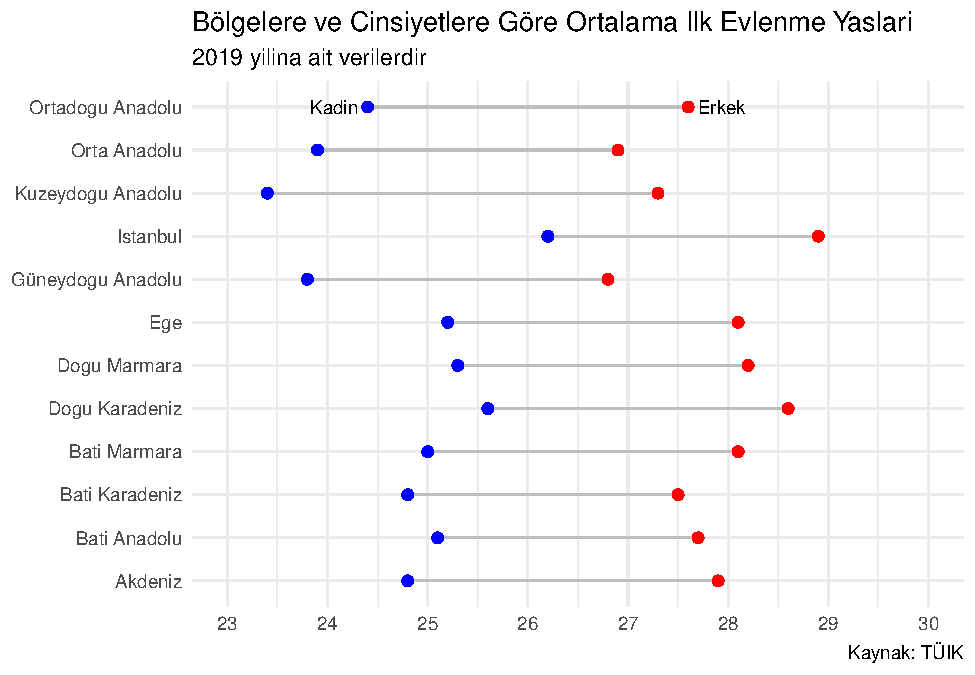
\includegraphics{rViz_files/figure-latex/unnamed-chunk-45-1.pdf}

\hypertarget{heatmap-isux131-haritasux131}{%
\section{Heatmap (Isı Haritası)}\label{heatmap-isux131-haritasux131}}

\emph{Tüketici güven endeksi:}

\begin{Shaded}
\begin{Highlighting}[]
\NormalTok{v16 }\OperatorTok\StringTok{ }
\StringTok{  }\KeywordTok{mutate}\NormalTok{(}\StringTok{"Yıl"}\NormalTok{ =}\StringTok{ }\KeywordTok{year}\NormalTok{(Tarih), }\StringTok{"Ay"}\NormalTok{ =}\StringTok{ }\KeywordTok{month}\NormalTok{(Tarih, }\DataTypeTok{label =} \OtherTok{TRUE}\NormalTok{))}

\CommentTok{#En basit şekilde}

\KeywordTok{ggplot}\NormalTok{(}\DataTypeTok{data =}\NormalTok{ v16) }\OperatorTok{+}
\StringTok{  }\KeywordTok{geom_tile}\NormalTok{(}\DataTypeTok{mapping =} \KeywordTok{aes}\NormalTok{(}\DataTypeTok{x =} \StringTok{`}\DataTypeTok{Yıl}\StringTok{`}\NormalTok{, }\DataTypeTok{y =}\NormalTok{ Ay, }\DataTypeTok{fill =}\NormalTok{ Endeks))}
\end{Highlighting}
\end{Shaded}

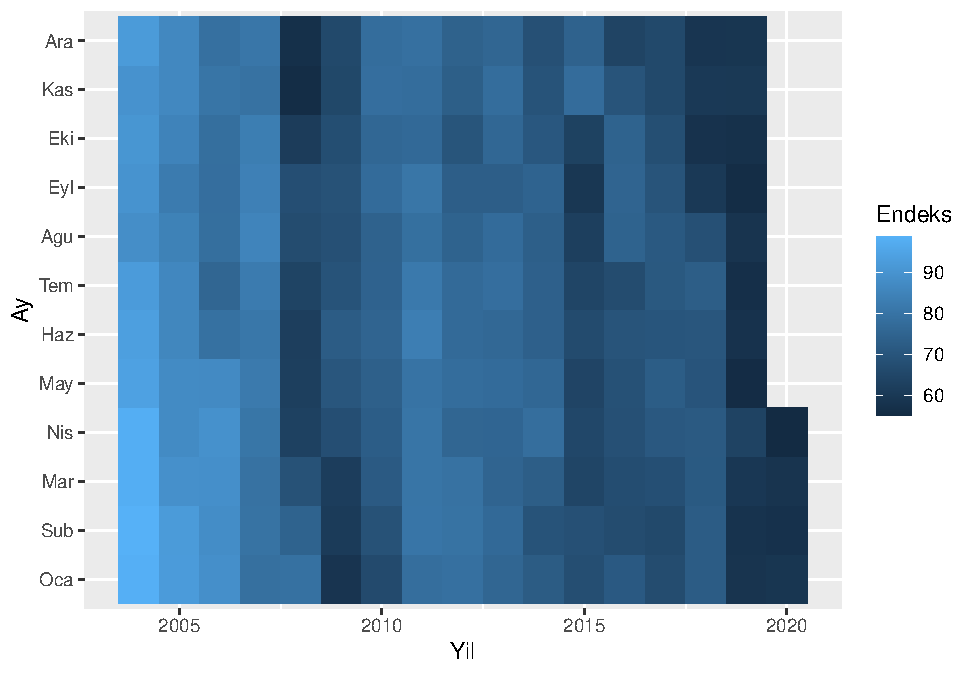
\includegraphics{rViz_files/figure-latex/unnamed-chunk-46-1.pdf}

\begin{itemize}
\tightlist
\item
  Renkleri değiştirebiliriz.
\end{itemize}

\begin{Shaded}
\begin{Highlighting}[]
\KeywordTok{ggplot}\NormalTok{(}\DataTypeTok{data =}\NormalTok{ v16) }\OperatorTok{+}
\StringTok{  }\KeywordTok{geom_tile}\NormalTok{(}\DataTypeTok{mapping =} \KeywordTok{aes}\NormalTok{(}\DataTypeTok{x =} \StringTok{`}\DataTypeTok{Yıl}\StringTok{`}\NormalTok{, }\DataTypeTok{y =}\NormalTok{ Ay, }\DataTypeTok{fill =}\NormalTok{ Endeks)) }\OperatorTok{+}
\StringTok{  }\KeywordTok{scale_fill_viridis_c}\NormalTok{()}
\end{Highlighting}
\end{Shaded}

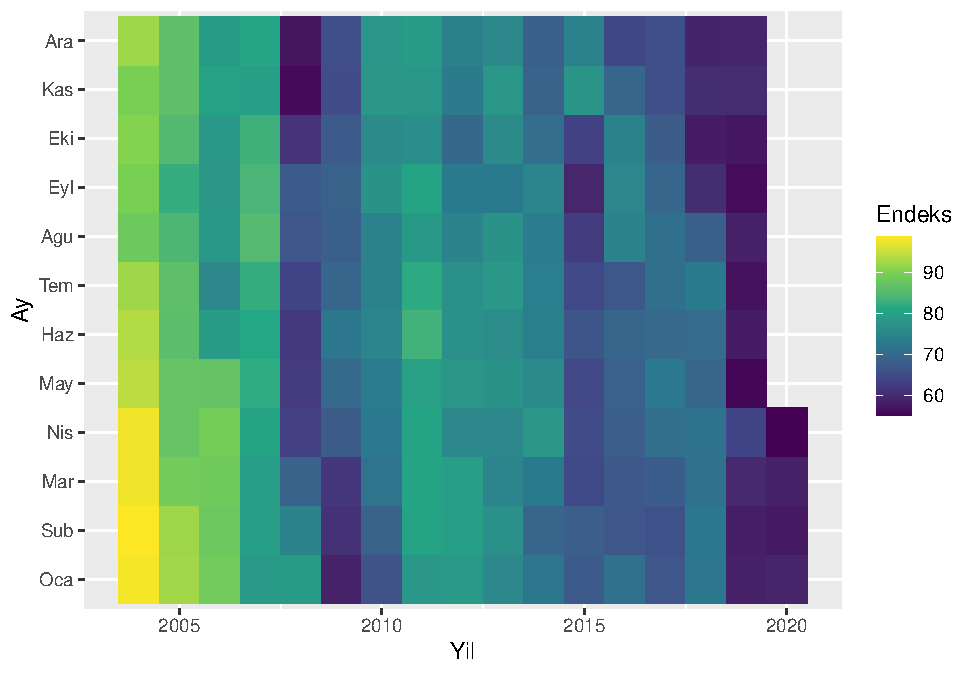
\includegraphics{rViz_files/figure-latex/unnamed-chunk-47-1.pdf}

\begin{itemize}
\item
  y eksenini ters çevirebiliriz.
\item
  Grafikteki boşlukları kapatabiliriz.
\end{itemize}

\begin{Shaded}
\begin{Highlighting}[]
\KeywordTok{ggplot}\NormalTok{(}\DataTypeTok{data =}\NormalTok{ v16) }\OperatorTok{+}
\StringTok{  }\KeywordTok{geom_tile}\NormalTok{(}\DataTypeTok{mapping =} \KeywordTok{aes}\NormalTok{(}\DataTypeTok{x =} \StringTok{`}\DataTypeTok{Yıl}\StringTok{`}\NormalTok{, }\DataTypeTok{y =}\NormalTok{ Ay, }\DataTypeTok{fill =}\NormalTok{ Endeks)) }\OperatorTok{+}
\StringTok{  }\KeywordTok{scale_fill_viridis_c}\NormalTok{() }\OperatorTok{+}
\StringTok{  }\KeywordTok{scale_y_discrete}\NormalTok{(}\DataTypeTok{limits =} \KeywordTok{rev}\NormalTok{(}\KeywordTok{levels}\NormalTok{(v16}\OperatorTok{$}\NormalTok{Ay))) }\OperatorTok{+}
\StringTok{  }\KeywordTok{scale_x_continuous}\NormalTok{(}\DataTypeTok{expand =} \KeywordTok{c}\NormalTok{(}\DecValTok{0}\NormalTok{,}\DecValTok{0}\NormalTok{))}
\end{Highlighting}
\end{Shaded}

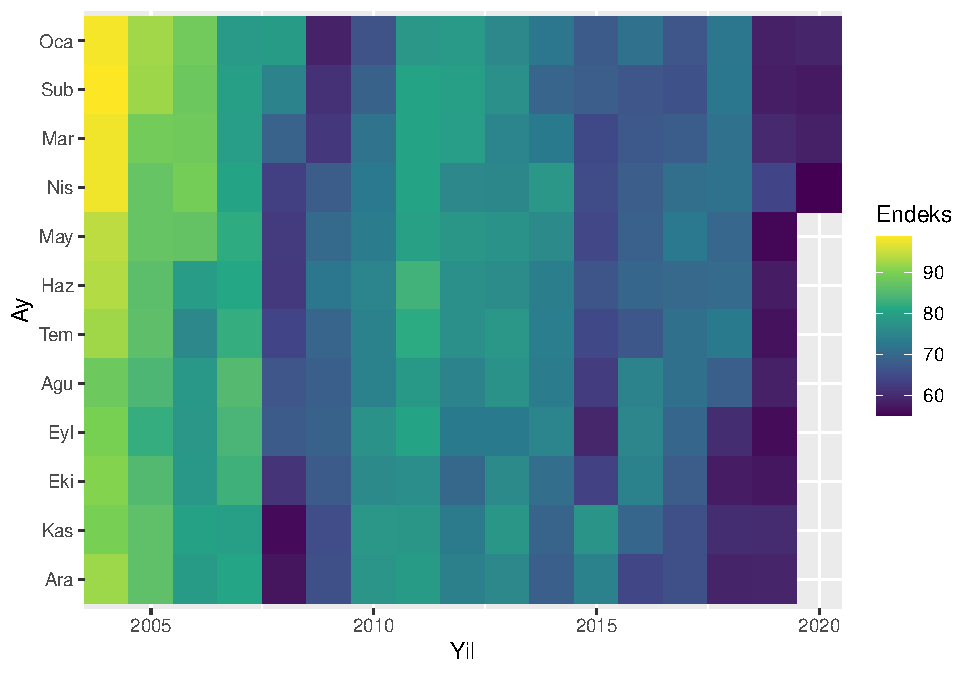
\includegraphics{rViz_files/figure-latex/unnamed-chunk-48-1.pdf}

\begin{itemize}
\item
  Lejantı düzenleyebiliriz.
\item
  x ve y eksenlerine ait başlıkları kaldırabiliriz.
\item
  Başlık, alt başlık ve kaynak ekleyebiliriz.
\item
  Temayı değiştirebiliriz.
\end{itemize}

\begin{Shaded}
\begin{Highlighting}[]
\KeywordTok{ggplot}\NormalTok{(}\DataTypeTok{data =}\NormalTok{ v16) }\OperatorTok{+}
\StringTok{  }\KeywordTok{geom_tile}\NormalTok{(}\DataTypeTok{mapping =} \KeywordTok{aes}\NormalTok{(}\DataTypeTok{x =} \StringTok{`}\DataTypeTok{Yıl}\StringTok{`}\NormalTok{, }\DataTypeTok{y =}\NormalTok{ Ay, }\DataTypeTok{fill =}\NormalTok{ Endeks)) }\OperatorTok{+}
\StringTok{  }\KeywordTok{scale_fill_viridis_c}\NormalTok{() }\OperatorTok{+}
\StringTok{  }\KeywordTok{theme}\NormalTok{(}\DataTypeTok{legend.position =} \StringTok{"bottom"}\NormalTok{,}
        \DataTypeTok{legend.key.width =} \KeywordTok{unit}\NormalTok{(}\DecValTok{3}\NormalTok{, }\StringTok{"cm"}\NormalTok{),}
        \DataTypeTok{legend.title =} \KeywordTok{element_blank}\NormalTok{(),}
        \DataTypeTok{panel.background =} \KeywordTok{element_rect}\NormalTok{(}\DataTypeTok{fill =} \StringTok{"white"}\NormalTok{, }\DataTypeTok{colour =} \StringTok{"gray"}\NormalTok{)) }\OperatorTok{+}
\StringTok{  }\KeywordTok{scale_y_discrete}\NormalTok{(}\DataTypeTok{limits =} \KeywordTok{rev}\NormalTok{(}\KeywordTok{levels}\NormalTok{(v16}\OperatorTok{$}\NormalTok{Ay))) }\OperatorTok{+}
\StringTok{  }\KeywordTok{scale_x_continuous}\NormalTok{(}\DataTypeTok{expand =} \KeywordTok{c}\NormalTok{(}\DecValTok{0}\NormalTok{,}\DecValTok{0}\NormalTok{)) }\OperatorTok{+}
\StringTok{  }\KeywordTok{labs}\NormalTok{(}\DataTypeTok{x =} \OtherTok{NULL}\NormalTok{,}
       \DataTypeTok{y =} \OtherTok{NULL}\NormalTok{,}
       \DataTypeTok{title =} \StringTok{"Tüketici Güven Endeksi"}\NormalTok{,}
       \DataTypeTok{subtitle =} \StringTok{"Ocak/2004-Nisan/2020 tarihlerine ait verilerdir"}\NormalTok{,}
       \DataTypeTok{caption =} \StringTok{"Kaynak: TÜİK"}\NormalTok{)}
\end{Highlighting}
\end{Shaded}

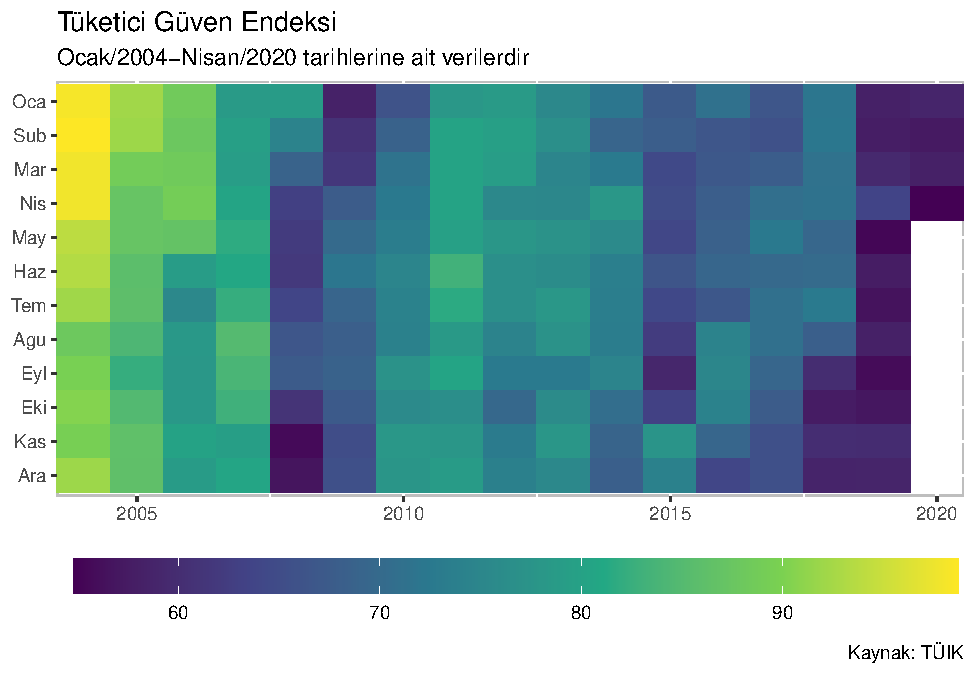
\includegraphics{rViz_files/figure-latex/unnamed-chunk-49-1.pdf}

\hypertarget{histogram}{%
\section{Histogram}\label{histogram}}

\emph{Günlük BIST Endeksi toplam işlem hacmi:}

\begin{Shaded}
\begin{Highlighting}[]
\CommentTok{#En basit şekilde}

\KeywordTok{ggplot}\NormalTok{(}\DataTypeTok{data =}\NormalTok{ v17) }\OperatorTok{+}
\StringTok{  }\KeywordTok{geom_histogram}\NormalTok{(}\DataTypeTok{mapping =} \KeywordTok{aes}\NormalTok{(}\DataTypeTok{x =} \StringTok{`}\DataTypeTok{ToplamİşlemHacmi}\StringTok{`}\NormalTok{))}
\end{Highlighting}
\end{Shaded}

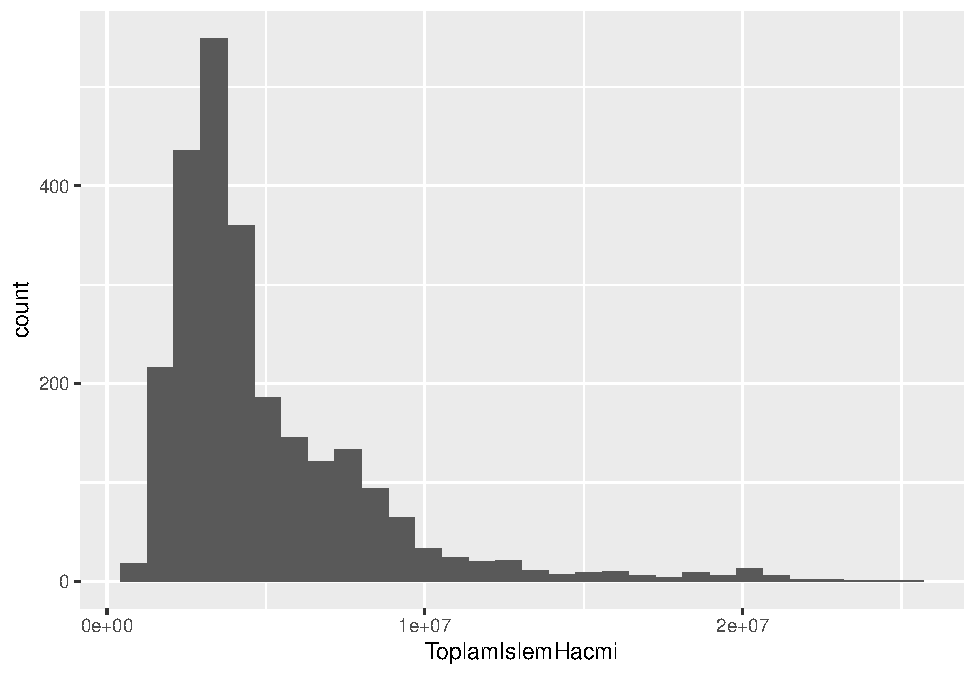
\includegraphics{rViz_files/figure-latex/unnamed-chunk-50-1.pdf}

\begin{itemize}
\item
  Aralık seçimini ayarlayabiliriz.
\item
  x eksenine ait değerleri daha okunabilir bir formata getirebiliriz.
\item
  Renklendirme yapabiliriz.
\end{itemize}

\begin{Shaded}
\begin{Highlighting}[]
\KeywordTok{ggplot}\NormalTok{(}\DataTypeTok{data =}\NormalTok{ v17) }\OperatorTok{+}
\StringTok{  }\KeywordTok{geom_histogram}\NormalTok{(}\DataTypeTok{mapping =} \KeywordTok{aes}\NormalTok{(}\DataTypeTok{x =} \StringTok{`}\DataTypeTok{ToplamİşlemHacmi}\StringTok{`}\NormalTok{), }\DataTypeTok{binwidth =} \DecValTok{500000}\NormalTok{, }\DataTypeTok{fill =} \StringTok{"dark red"}\NormalTok{) }\OperatorTok{+}
\StringTok{  }\KeywordTok{scale_x_continuous}\NormalTok{(}\DataTypeTok{labels =}\NormalTok{ comma)}
\end{Highlighting}
\end{Shaded}

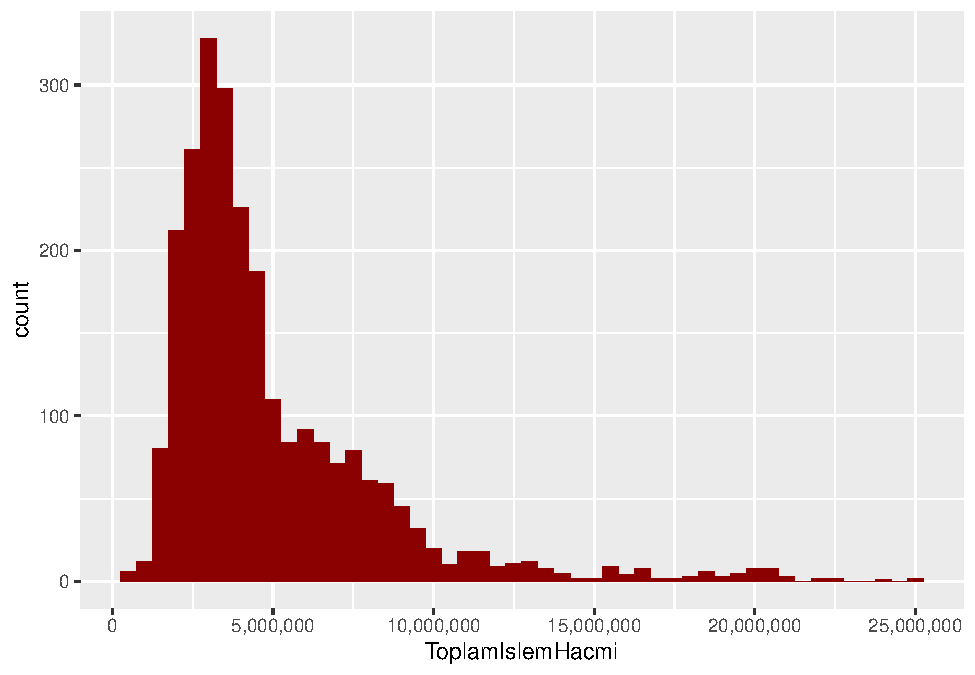
\includegraphics{rViz_files/figure-latex/unnamed-chunk-51-1.pdf}

\begin{itemize}
\item
  x eksenine ait başlığı kaldırabilir, y eksenine ait başlığı düzeltebiliriz.
\item
  Ortalama çizgisi (kesikli) ekleyebiliriz.
\item
  Başlık, alt başlık ve kaynak ekleyebiliriz.
\item
  Temayı değiştirebiliriz.
\end{itemize}

\begin{Shaded}
\begin{Highlighting}[]
\KeywordTok{ggplot}\NormalTok{(}\DataTypeTok{data =}\NormalTok{ v17) }\OperatorTok{+}
\StringTok{  }\KeywordTok{geom_histogram}\NormalTok{(}\DataTypeTok{mapping =} \KeywordTok{aes}\NormalTok{(}\DataTypeTok{x =} \StringTok{`}\DataTypeTok{ToplamİşlemHacmi}\StringTok{`}\NormalTok{), }\DataTypeTok{binwidth =} \DecValTok{500000}\NormalTok{, }\DataTypeTok{fill =} \StringTok{"dark red"}\NormalTok{) }\OperatorTok{+}
\StringTok{  }\KeywordTok{geom_vline}\NormalTok{(}\DataTypeTok{xintercept =} \KeywordTok{mean}\NormalTok{(v17}\OperatorTok{$}\StringTok{`}\DataTypeTok{ToplamİşlemHacmi}\StringTok{`}\NormalTok{), }\DataTypeTok{linetype =} \StringTok{"dashed"}\NormalTok{) }\OperatorTok{+}
\StringTok{  }\KeywordTok{theme_minimal}\NormalTok{() }\OperatorTok{+}
\StringTok{  }\KeywordTok{scale_x_continuous}\NormalTok{(}\DataTypeTok{labels =}\NormalTok{ comma) }\OperatorTok{+}
\StringTok{  }\KeywordTok{labs}\NormalTok{(}\DataTypeTok{x =} \OtherTok{NULL}\NormalTok{,}
       \DataTypeTok{y =} \StringTok{"Sayma"}\NormalTok{,}
       \DataTypeTok{title =} \StringTok{"Günlük BIST Endeksi Toplam İşlem Hacmi"}\NormalTok{,}
       \DataTypeTok{subtitle =} \StringTok{"Son 10 yıla ait verilerdir"}\NormalTok{,}
       \DataTypeTok{caption =} \StringTok{"Kaynak: TCMB"}\NormalTok{)}
\end{Highlighting}
\end{Shaded}

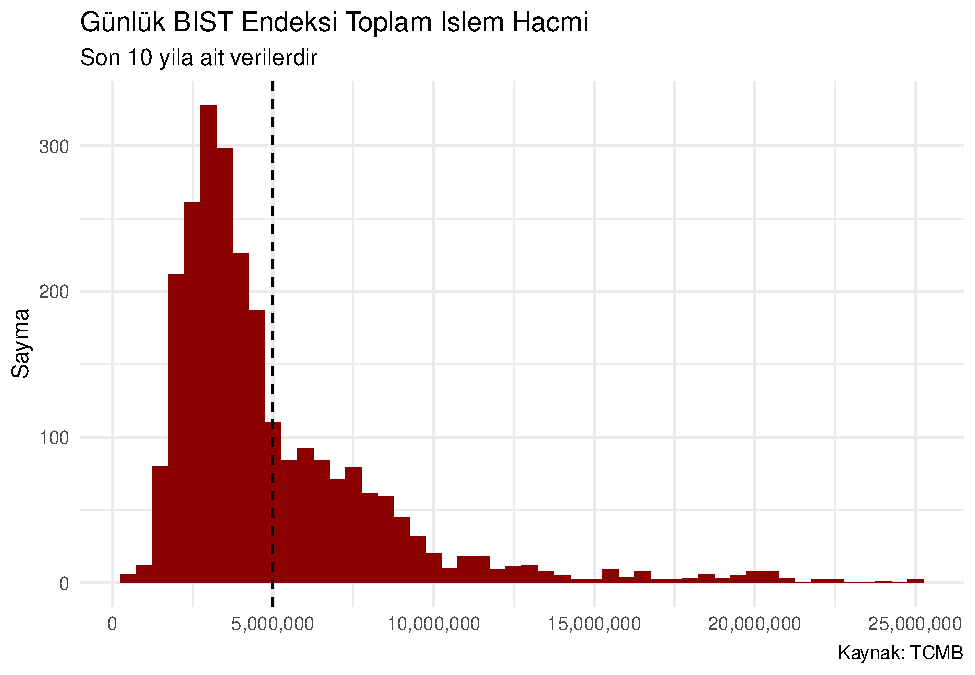
\includegraphics{rViz_files/figure-latex/unnamed-chunk-52-1.pdf}

\hypertarget{line-uxe7izgi}{%
\section{Line (Çizgi)}\label{line-uxe7izgi}}

\emph{Günlük Dolar ve Euro alış kuru:}

\begin{Shaded}
\begin{Highlighting}[]
\NormalTok{v18 }\OperatorTok\StringTok{ }
\StringTok{  }\KeywordTok{mutate}\NormalTok{(}\DataTypeTok{Tarih =} \KeywordTok{as.Date}\NormalTok{(Tarih))}

\CommentTok{#En basit şekilde}

\KeywordTok{ggplot}\NormalTok{(}\DataTypeTok{data =}\NormalTok{ v18) }\OperatorTok{+}
\StringTok{  }\KeywordTok{geom_line}\NormalTok{(}\DataTypeTok{mapping =} \KeywordTok{aes}\NormalTok{(}\DataTypeTok{x =}\NormalTok{ Tarih, }\DataTypeTok{y =} \StringTok{`}\DataTypeTok{Alış}\StringTok{`}\NormalTok{, }\DataTypeTok{group =}\NormalTok{ Kur))}
\end{Highlighting}
\end{Shaded}

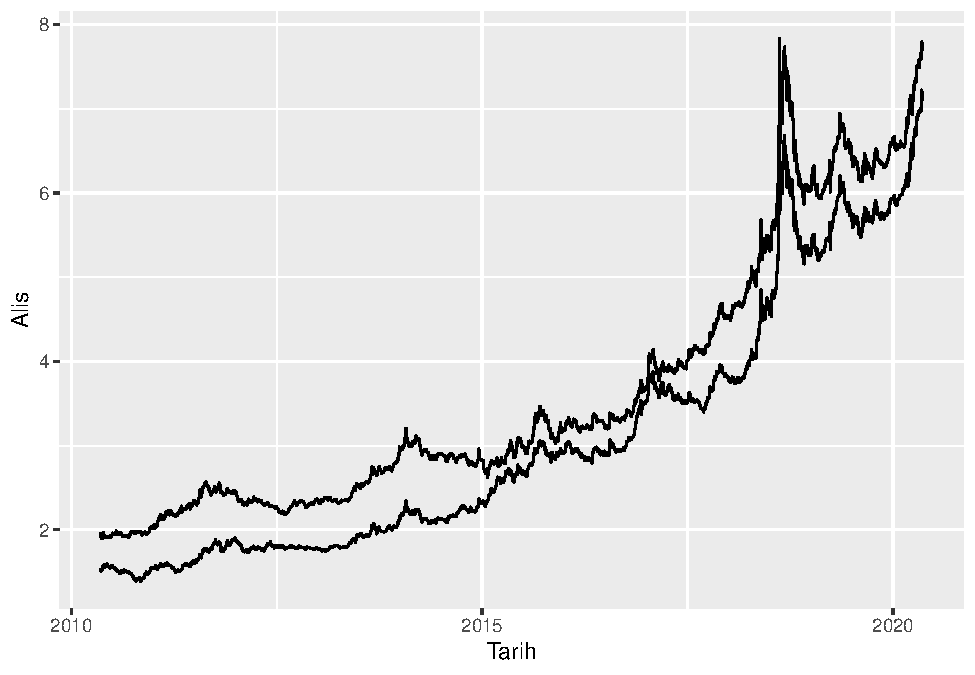
\includegraphics{rViz_files/figure-latex/unnamed-chunk-53-1.pdf}

\begin{itemize}
\item
  Renkleri değiştirebiliriz.
\item
  Kur tiplerini ayırabiliriz.
\item
  x eksenindeki tarihleri belli bir aralıkta gösterebiliriz.
\item
  y eksenindeki değerleri belli bir limit ve aralıkta gösterebiliriz.
\end{itemize}

\begin{Shaded}
\begin{Highlighting}[]
\KeywordTok{ggplot}\NormalTok{(}\DataTypeTok{data =}\NormalTok{ v18) }\OperatorTok{+}
\StringTok{  }\KeywordTok{geom_line}\NormalTok{(}\DataTypeTok{mapping =} \KeywordTok{aes}\NormalTok{(}\DataTypeTok{x=}\NormalTok{ Tarih, }\DataTypeTok{y =} \StringTok{`}\DataTypeTok{Alış}\StringTok{`}\NormalTok{, }\DataTypeTok{group =}\NormalTok{ Kur, }\DataTypeTok{color =}\NormalTok{ Kur)) }\OperatorTok{+}
\StringTok{  }\KeywordTok{scale_x_date}\NormalTok{(}\DataTypeTok{date_labels =} \StringTok{"%Y"}\NormalTok{, }\DataTypeTok{date_breaks =} \StringTok{"year"}\NormalTok{) }\OperatorTok{+}
\StringTok{  }\KeywordTok{scale_y_continuous}\NormalTok{(}\DataTypeTok{limits =} \KeywordTok{c}\NormalTok{(}\DecValTok{0}\NormalTok{,}\DecValTok{8}\NormalTok{), }\DataTypeTok{breaks =} \KeywordTok{seq}\NormalTok{(}\DecValTok{0}\NormalTok{,}\DecValTok{8}\NormalTok{,}\DecValTok{1}\NormalTok{)) }\OperatorTok{+}
\StringTok{  }\KeywordTok{scale_color_manual}\NormalTok{(}\DataTypeTok{values =} \KeywordTok{c}\NormalTok{(}\StringTok{"black"}\NormalTok{,}\StringTok{"red"}\NormalTok{))}
\end{Highlighting}
\end{Shaded}

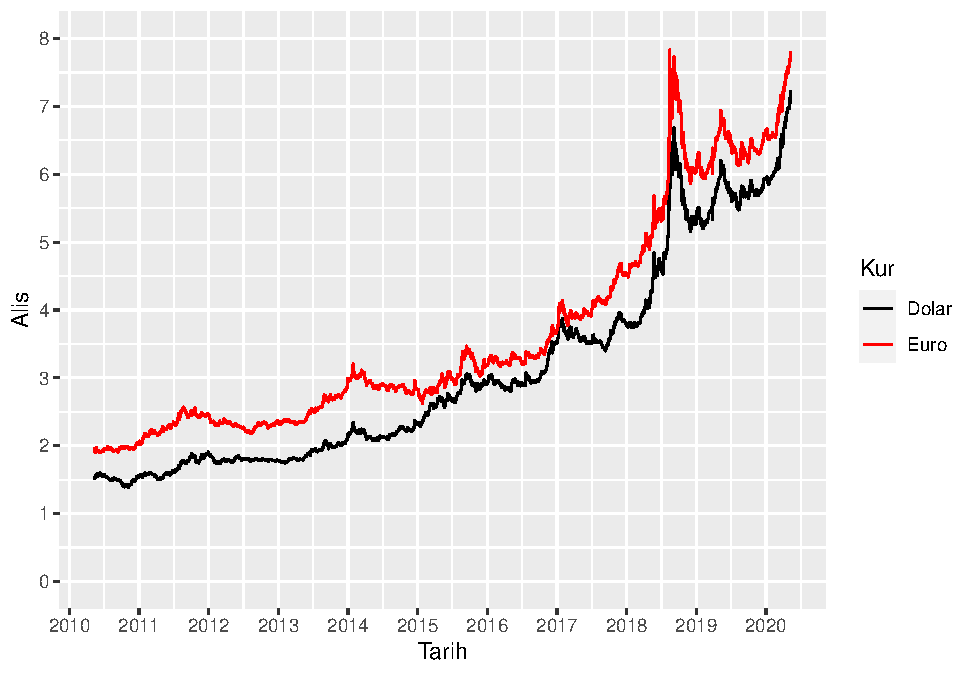
\includegraphics{rViz_files/figure-latex/unnamed-chunk-54-1.pdf}

\begin{itemize}
\tightlist
\item
  Her bir çizginin sonunda hangi kura ait olduğunu belirtebiliriz.
\end{itemize}

\begin{Shaded}
\begin{Highlighting}[]
\KeywordTok{ggplot}\NormalTok{(}\DataTypeTok{data =}\NormalTok{ v18, }\DataTypeTok{mapping =} \KeywordTok{aes}\NormalTok{(}\DataTypeTok{x=}\NormalTok{ Tarih, }\DataTypeTok{y =} \StringTok{`}\DataTypeTok{Alış}\StringTok{`}\NormalTok{, }\DataTypeTok{group =}\NormalTok{ Kur, }\DataTypeTok{color =}\NormalTok{ Kur)) }\OperatorTok{+}
\StringTok{  }\KeywordTok{geom_line}\NormalTok{() }\OperatorTok{+}
\StringTok{  }\KeywordTok{geom_dl}\NormalTok{(}\KeywordTok{aes}\NormalTok{(}\DataTypeTok{label =}\NormalTok{ Kur), }\DataTypeTok{method =} \KeywordTok{list}\NormalTok{(}\KeywordTok{dl.combine}\NormalTok{(}\StringTok{"last.points"}\NormalTok{), }\DataTypeTok{cex =} \FloatTok{0.8}\NormalTok{)) }\OperatorTok{+}
\StringTok{  }\KeywordTok{scale_x_date}\NormalTok{(}\DataTypeTok{date_labels =} \StringTok{"%Y"}\NormalTok{, }\DataTypeTok{date_breaks =} \StringTok{"year"}\NormalTok{) }\OperatorTok{+}
\StringTok{  }\KeywordTok{scale_y_continuous}\NormalTok{(}\DataTypeTok{limits =} \KeywordTok{c}\NormalTok{(}\DecValTok{0}\NormalTok{,}\DecValTok{8}\NormalTok{), }\DataTypeTok{breaks =} \KeywordTok{seq}\NormalTok{(}\DecValTok{0}\NormalTok{,}\DecValTok{8}\NormalTok{,}\DecValTok{1}\NormalTok{)) }\OperatorTok{+}
\StringTok{  }\KeywordTok{scale_color_manual}\NormalTok{(}\DataTypeTok{values =} \KeywordTok{c}\NormalTok{(}\StringTok{"black"}\NormalTok{,}\StringTok{"red"}\NormalTok{))}
\end{Highlighting}
\end{Shaded}

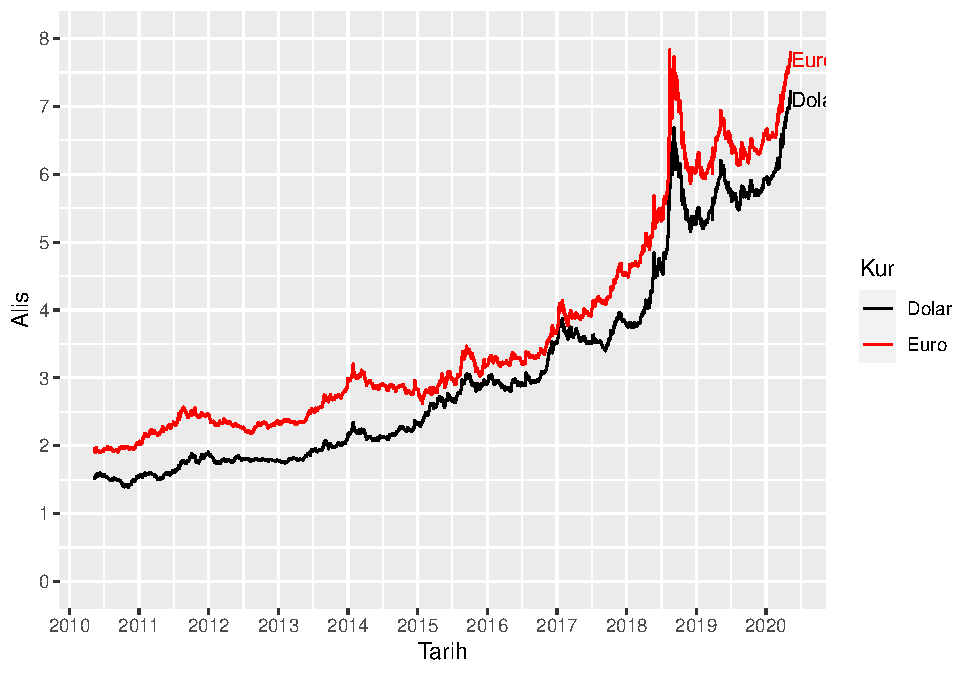
\includegraphics{rViz_files/figure-latex/unnamed-chunk-55-1.pdf}

\begin{itemize}
\item
  Lejantı kaldırabiliriz.
\item
  x eksenine ait başlığı kaldırabilir; y eksenine ait başlığı düzeltebiliriz.
\item
  Başlık, alt başlık ve kaynak ekleyebiliriz.
\item
  Temayı değiştirebiliriz.
\end{itemize}

\begin{Shaded}
\begin{Highlighting}[]
\KeywordTok{ggplot}\NormalTok{(}\DataTypeTok{data =}\NormalTok{ v18, }\DataTypeTok{mapping =} \KeywordTok{aes}\NormalTok{(}\DataTypeTok{x =}\NormalTok{ Tarih, }\DataTypeTok{y =} \StringTok{`}\DataTypeTok{Alış}\StringTok{`}\NormalTok{, }\DataTypeTok{group =}\NormalTok{ Kur, }\DataTypeTok{color =}\NormalTok{ Kur)) }\OperatorTok{+}
\StringTok{  }\KeywordTok{geom_line}\NormalTok{() }\OperatorTok{+}
\StringTok{  }\KeywordTok{geom_dl}\NormalTok{(}\KeywordTok{aes}\NormalTok{(}\DataTypeTok{label =}\NormalTok{ Kur), }\DataTypeTok{method =} \KeywordTok{list}\NormalTok{(}\KeywordTok{dl.combine}\NormalTok{(}\StringTok{"last.points"}\NormalTok{), }\DataTypeTok{cex =} \FloatTok{0.7}\NormalTok{)) }\OperatorTok{+}
\StringTok{  }\KeywordTok{theme_minimal}\NormalTok{() }\OperatorTok{+}
\StringTok{  }\KeywordTok{scale_x_date}\NormalTok{(}\DataTypeTok{date_labels =} \StringTok{"%Y"}\NormalTok{, }\DataTypeTok{date_breaks =} \StringTok{"year"}\NormalTok{) }\OperatorTok{+}
\StringTok{  }\KeywordTok{scale_y_continuous}\NormalTok{(}\DataTypeTok{limits =} \KeywordTok{c}\NormalTok{(}\DecValTok{0}\NormalTok{,}\DecValTok{8}\NormalTok{), }\DataTypeTok{breaks =} \KeywordTok{seq}\NormalTok{(}\DecValTok{0}\NormalTok{,}\DecValTok{8}\NormalTok{,}\DecValTok{1}\NormalTok{)) }\OperatorTok{+}
\StringTok{  }\KeywordTok{scale_color_manual}\NormalTok{(}\DataTypeTok{values =} \KeywordTok{c}\NormalTok{(}\StringTok{"black"}\NormalTok{,}\StringTok{"red"}\NormalTok{)) }\OperatorTok{+}
\StringTok{  }\KeywordTok{theme}\NormalTok{(}\DataTypeTok{legend.position =} \StringTok{"none"}\NormalTok{) }\OperatorTok{+}
\StringTok{  }\KeywordTok{labs}\NormalTok{(}\DataTypeTok{x =} \OtherTok{NULL}\NormalTok{,}
       \DataTypeTok{y =} \StringTok{"Alış"}\NormalTok{,}
       \DataTypeTok{title =} \StringTok{"Günlük Dolar ve Euro Alış Kuru"}\NormalTok{,}
       \DataTypeTok{subtitle =} \StringTok{"Son 10 yıla ait verilerdir"}\NormalTok{,}
       \DataTypeTok{caption =} \StringTok{"Kaynak: TCMB"}\NormalTok{)}
\end{Highlighting}
\end{Shaded}

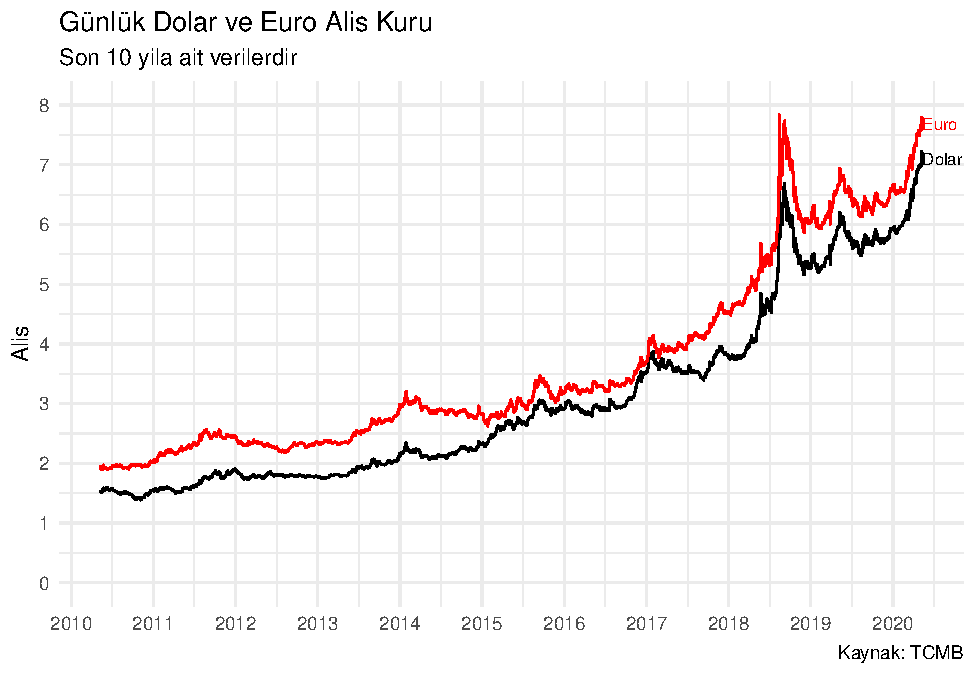
\includegraphics{rViz_files/figure-latex/unnamed-chunk-56-1.pdf}

\hypertarget{lollipop}{%
\section{Lollipop}\label{lollipop}}

\emph{Trafiğe kaydı yapılan otomobillerin renkleri:}

\begin{Shaded}
\begin{Highlighting}[]
\NormalTok{v9 }\OperatorTok\StringTok{ }
\StringTok{  }\KeywordTok{filter}\NormalTok{(Renk }\OperatorTok{!=}\StringTok{ "Diğer"}\NormalTok{)}

\CommentTok{#En basit şekilde}

\KeywordTok{ggplot}\NormalTok{(}\DataTypeTok{data =}\NormalTok{ v9, }\DataTypeTok{mapping =} \KeywordTok{aes}\NormalTok{(}\DataTypeTok{x =}\NormalTok{ Renk, }\DataTypeTok{y =} \StringTok{`}\DataTypeTok{OtomobilSayısı}\StringTok{`}\NormalTok{)) }\OperatorTok{+}
\StringTok{  }\KeywordTok{geom_segment}\NormalTok{(}\DataTypeTok{mapping =} \KeywordTok{aes}\NormalTok{(}\DataTypeTok{xend =}\NormalTok{ Renk, }\DataTypeTok{y =} \DecValTok{0}\NormalTok{, }\DataTypeTok{yend =} \StringTok{`}\DataTypeTok{OtomobilSayısı}\StringTok{`}\NormalTok{)) }\OperatorTok{+}
\StringTok{  }\KeywordTok{geom_point}\NormalTok{()}
\end{Highlighting}
\end{Shaded}

\includegraphics{rViz_files/figure-latex/unnamed-chunk-57-1.pdf}

\begin{itemize}
\item
  Çizgileri kesikli yapabiliriz.
\item
  Noktaların renklerini ve büyüklüklerini değiştirebiliriz.
\item
  Büyükten küçüğe sıralayabiliriz.
\item
  x eksenine ait değerleri daha okunabilir bir formata getirebiliriz.
\end{itemize}

\begin{Shaded}
\begin{Highlighting}[]
\KeywordTok{ggplot}\NormalTok{(}\DataTypeTok{data =}\NormalTok{ v9, }\DataTypeTok{mapping =} \KeywordTok{aes}\NormalTok{(}\DataTypeTok{x =} \KeywordTok{reorder}\NormalTok{(Renk, }\OperatorTok{-}\StringTok{`}\DataTypeTok{OtomobilSayısı}\StringTok{`}\NormalTok{), }\DataTypeTok{y =} \StringTok{`}\DataTypeTok{OtomobilSayısı}\StringTok{`}\NormalTok{)) }\OperatorTok{+}
\StringTok{  }\KeywordTok{geom_segment}\NormalTok{(}\DataTypeTok{mapping =} \KeywordTok{aes}\NormalTok{(}\DataTypeTok{xend =}\NormalTok{ Renk, }\DataTypeTok{y =} \DecValTok{0}\NormalTok{, }\DataTypeTok{yend =} \StringTok{`}\DataTypeTok{OtomobilSayısı}\StringTok{`}\NormalTok{), }\DataTypeTok{linetype =} \StringTok{"dashed"}\NormalTok{) }\OperatorTok{+}
\StringTok{  }\KeywordTok{geom_point}\NormalTok{(}\DataTypeTok{size =} \DecValTok{3}\NormalTok{, }\DataTypeTok{mapping =} \KeywordTok{aes}\NormalTok{(}\DataTypeTok{color =}\NormalTok{ Renk)) }\OperatorTok{+}
\StringTok{  }\KeywordTok{scale_y_continuous}\NormalTok{(}\DataTypeTok{labels =}\NormalTok{ comma) }\OperatorTok{+}
\StringTok{  }\KeywordTok{scale_color_manual}\NormalTok{(}\DataTypeTok{values =} \KeywordTok{c}\NormalTok{(}\StringTok{"white"}\NormalTok{,}\StringTok{"gray"}\NormalTok{,}\StringTok{"brown"}\NormalTok{,}\StringTok{"red"}\NormalTok{,}\StringTok{"blue"}\NormalTok{,}\StringTok{"yellow"}\NormalTok{,}\StringTok{"black"}\NormalTok{,}\StringTok{"orange"}\NormalTok{,}\StringTok{"green"}\NormalTok{))}
\end{Highlighting}
\end{Shaded}

\includegraphics{rViz_files/figure-latex/unnamed-chunk-58-1.pdf}

\begin{itemize}
\item
  x eksenine ait başlığı kaldırabilir; y eksenine ait başlığı düzeltebiliriz.
\item
  Lejantı kaldırabiliriz.
\item
  Başlık, alt başlık ve kaynak ekleyebiliriz.
\item
  Temayı değiştirebiliriz.
\end{itemize}

\begin{Shaded}
\begin{Highlighting}[]
\KeywordTok{ggplot}\NormalTok{(}\DataTypeTok{data =}\NormalTok{ v9, }\DataTypeTok{mapping =} \KeywordTok{aes}\NormalTok{(}\DataTypeTok{x =} \KeywordTok{reorder}\NormalTok{(Renk, }\OperatorTok{-}\StringTok{`}\DataTypeTok{OtomobilSayısı}\StringTok{`}\NormalTok{), }\DataTypeTok{y =} \StringTok{`}\DataTypeTok{OtomobilSayısı}\StringTok{`}\NormalTok{)) }\OperatorTok{+}
\StringTok{  }\KeywordTok{geom_segment}\NormalTok{(}\DataTypeTok{mapping =} \KeywordTok{aes}\NormalTok{(}\DataTypeTok{xend =}\NormalTok{ Renk, }\DataTypeTok{y =} \DecValTok{0}\NormalTok{, }\DataTypeTok{yend =} \StringTok{`}\DataTypeTok{OtomobilSayısı}\StringTok{`}\NormalTok{), }\DataTypeTok{linetype =} \StringTok{"dashed"}\NormalTok{) }\OperatorTok{+}
\StringTok{  }\KeywordTok{geom_point}\NormalTok{(}\DataTypeTok{size =} \DecValTok{5}\NormalTok{, }\DataTypeTok{mapping =} \KeywordTok{aes}\NormalTok{(}\DataTypeTok{color =}\NormalTok{ Renk)) }\OperatorTok{+}
\StringTok{  }\KeywordTok{theme_dark}\NormalTok{() }\OperatorTok{+}
\StringTok{  }\KeywordTok{theme}\NormalTok{(}\DataTypeTok{legend.position =} \StringTok{"none"}\NormalTok{) }\OperatorTok{+}
\StringTok{  }\KeywordTok{scale_y_continuous}\NormalTok{(}\DataTypeTok{labels =}\NormalTok{ comma) }\OperatorTok{+}
\StringTok{  }\KeywordTok{scale_color_manual}\NormalTok{(}\DataTypeTok{values =} \KeywordTok{c}\NormalTok{(}\StringTok{"white"}\NormalTok{,}\StringTok{"gray"}\NormalTok{,}\StringTok{"brown"}\NormalTok{,}\StringTok{"red"}\NormalTok{,}\StringTok{"blue"}\NormalTok{,}\StringTok{"yellow"}\NormalTok{,}\StringTok{"black"}\NormalTok{,}\StringTok{"orange"}\NormalTok{,}\StringTok{"green"}\NormalTok{)) }\OperatorTok{+}
\StringTok{  }\KeywordTok{labs}\NormalTok{(}\DataTypeTok{x =} \OtherTok{NULL}\NormalTok{,}
       \DataTypeTok{y =} \StringTok{"Otomobil Sayısı"}\NormalTok{,}
       \DataTypeTok{title =} \StringTok{"Trafiğe Kaydı Yapılan Otomobillerin Renkleri"}\NormalTok{,}
       \DataTypeTok{subtitle =} \StringTok{"2020 yılına ait verilerdir"}\NormalTok{,}
       \DataTypeTok{caption =} \StringTok{"Kaynak: TÜİK"}\NormalTok{)}
\end{Highlighting}
\end{Shaded}

\includegraphics{rViz_files/figure-latex/unnamed-chunk-59-1.pdf}

\hypertarget{multi-set-bar-uxe7oklu-uxe7ubuk}{%
\section{Multi-set Bar (Çoklu Çubuk)}\label{multi-set-bar-uxe7oklu-uxe7ubuk}}

\emph{Bölgeler düzeyinde tiyatro-sinema seyirci sayısı:}

\begin{Shaded}
\begin{Highlighting}[]
\CommentTok{#En basit şekilde}

\KeywordTok{ggplot}\NormalTok{(}\DataTypeTok{data =}\NormalTok{ v19) }\OperatorTok{+}
\StringTok{  }\KeywordTok{geom_col}\NormalTok{(}\DataTypeTok{mapping =} \KeywordTok{aes}\NormalTok{(}\DataTypeTok{x =} \StringTok{`}\DataTypeTok{Bölge}\StringTok{`}\NormalTok{, }\DataTypeTok{y =} \StringTok{`}\DataTypeTok{Sayı}\StringTok{`}\NormalTok{, }\DataTypeTok{fill =} \StringTok{`}\DataTypeTok{Tip}\StringTok{`}\NormalTok{), }\DataTypeTok{position =} \StringTok{"dodge"}\NormalTok{)}
\end{Highlighting}
\end{Shaded}

\includegraphics{rViz_files/figure-latex/unnamed-chunk-60-1.pdf}

\begin{itemize}
\item
  x ekseninde yer alan bölge isimlerini küçültebiliriz.
\item
  y eksenine ait değerleri daha okunabilir bir formata getirebiliriz.
\item
  Çubukları büyükten küçüğe doğru sıralayabiliriz.
\item
  Çubukları renklendirebiliriz.
\end{itemize}

\begin{Shaded}
\begin{Highlighting}[]
\KeywordTok{ggplot}\NormalTok{(}\DataTypeTok{data =}\NormalTok{ v19) }\OperatorTok{+}
\StringTok{  }\KeywordTok{geom_col}\NormalTok{(}\DataTypeTok{mapping =} \KeywordTok{aes}\NormalTok{(}\DataTypeTok{x =} \KeywordTok{reorder}\NormalTok{(}\StringTok{`}\DataTypeTok{Bölge}\StringTok{`}\NormalTok{, }\OperatorTok{-}\StringTok{`}\DataTypeTok{Sayı}\StringTok{`}\NormalTok{), }\DataTypeTok{y =} \StringTok{`}\DataTypeTok{Sayı}\StringTok{`}\NormalTok{, }\DataTypeTok{fill =} \StringTok{`}\DataTypeTok{Tip}\StringTok{`}\NormalTok{), }\DataTypeTok{position =} \StringTok{"dodge"}\NormalTok{) }\OperatorTok{+}
\StringTok{  }\KeywordTok{theme}\NormalTok{(}\DataTypeTok{axis.text.x =} \KeywordTok{element_text}\NormalTok{(}\DataTypeTok{size =} \DecValTok{5}\NormalTok{)) }\OperatorTok{+}
\StringTok{  }\KeywordTok{scale_y_continuous}\NormalTok{(}\DataTypeTok{labels =}\NormalTok{ comma) }\OperatorTok{+}
\StringTok{  }\KeywordTok{scale_fill_manual}\NormalTok{(}\DataTypeTok{values =} \KeywordTok{c}\NormalTok{(}\StringTok{"red"}\NormalTok{,}\StringTok{"blue"}\NormalTok{))}
\end{Highlighting}
\end{Shaded}

\includegraphics{rViz_files/figure-latex/unnamed-chunk-61-1.pdf}

\begin{itemize}
\item
  Lejantı kaldırabiliriz.
\item
  x ve y eksenlerine ait başlıkları kaldırabiliriz.
\item
  Başlık, alt başlık ve kaynak ekleyebiliriz.
\item
  Temayı değiştirebiliriz.
\end{itemize}

\begin{Shaded}
\begin{Highlighting}[]
\KeywordTok{ggplot}\NormalTok{(}\DataTypeTok{data =}\NormalTok{ v19) }\OperatorTok{+}
\StringTok{  }\KeywordTok{geom_col}\NormalTok{(}\DataTypeTok{mapping =} \KeywordTok{aes}\NormalTok{(}\DataTypeTok{x =} \KeywordTok{reorder}\NormalTok{(}\StringTok{`}\DataTypeTok{Bölge}\StringTok{`}\NormalTok{, }\OperatorTok{-}\StringTok{`}\DataTypeTok{Sayı}\StringTok{`}\NormalTok{), }\DataTypeTok{y =} \StringTok{`}\DataTypeTok{Sayı}\StringTok{`}\NormalTok{, }\DataTypeTok{fill =} \StringTok{`}\DataTypeTok{Tip}\StringTok{`}\NormalTok{), }\DataTypeTok{position =} \StringTok{"dodge"}\NormalTok{) }\OperatorTok{+}
\StringTok{  }\KeywordTok{theme_minimal}\NormalTok{() }\OperatorTok{+}
\StringTok{  }\KeywordTok{scale_y_continuous}\NormalTok{(}\DataTypeTok{labels =}\NormalTok{ comma) }\OperatorTok{+}
\StringTok{  }\KeywordTok{theme}\NormalTok{(}\DataTypeTok{axis.text.x =} \KeywordTok{element_text}\NormalTok{(}\DataTypeTok{size =} \DecValTok{6}\NormalTok{),}
        \DataTypeTok{axis.title.x =} \KeywordTok{element_blank}\NormalTok{(),}
        \DataTypeTok{axis.title.y =} \KeywordTok{element_blank}\NormalTok{(),}
        \DataTypeTok{legend.position =} \StringTok{"bottom"}\NormalTok{,}
        \DataTypeTok{legend.title =} \KeywordTok{element_blank}\NormalTok{()) }\OperatorTok{+}
\StringTok{  }\KeywordTok{labs}\NormalTok{(}\DataTypeTok{title =} \StringTok{"Bölgeler Düzeyinde Tiyatro ve Sinema Seyirci Sayısı"}\NormalTok{,}
       \DataTypeTok{subtitle =} \StringTok{"2018 yılına ait verilerdir"}\NormalTok{,}
       \DataTypeTok{caption =} \StringTok{"Kaynak: TÜİK"}\NormalTok{) }\OperatorTok{+}
\StringTok{  }\KeywordTok{scale_fill_manual}\NormalTok{(}\DataTypeTok{values =} \KeywordTok{c}\NormalTok{(}\StringTok{"red"}\NormalTok{,}\StringTok{"blue"}\NormalTok{))}
\end{Highlighting}
\end{Shaded}

\includegraphics{rViz_files/figure-latex/unnamed-chunk-62-1.pdf}

\hypertarget{network-aux11f}{%
\section{Network (Ağ)}\label{network-aux11f}}

\emph{Seçtiğim dört arkadaş + benim ortak takip ettiğimiz hesaplar:}

\begin{Shaded}
\begin{Highlighting}[]
\KeywordTok{plot}\NormalTok{(}\KeywordTok{graph_from_data_frame}\NormalTok{(v20))}

\CommentTok{#Kişisel çalışmanızı aşağıdaki gibi yapabilirsiniz:}
\CommentTok{# library(rtweet)}
\CommentTok{# arkadaslar <- get_friends(c("EdaDenizOzdemir","canozkaaan","sam_econ","fratmelhylmaz","rpydaneogrendim"))}
\CommentTok{# tablo <- table(arkadaslar$user_id)}
\CommentTok{# arkadaslar <- subset(arkadaslar, user_id %in% names(tablo[tablo >= 4L]))}
\CommentTok{# isimler <- lookup_users(arkadaslar$user_id)}
\CommentTok{# isimler <- isimler[,c(1,4)]}
\CommentTok{# arkadaslar <- merge(arkadaslar, isimler[,-2], by = "user_id")}
\end{Highlighting}
\end{Shaded}

\includegraphics[width=1\linewidth]{C:/Users/datanerd/Desktop/Github/rViz/img/network}

\hypertarget{ohlc-auxe7ux131lux131ux15f-yuxfckseliux15f-duxfcux15fuxfcux15f-kapanux131ux15f}{%
\section{OHLC (Açılış-Yükseliş-Düşüş-Kapanış)}\label{ohlc-auxe7ux131lux131ux15f-yuxfckseliux15f-duxfcux15fuxfcux15f-kapanux131ux15f}}

\emph{BIST'e ait açılış, en yüksek, en düşük, kapanış değerleri:}

\begin{Shaded}
\begin{Highlighting}[]
\NormalTok{v6 }\OperatorTok\StringTok{ }
\StringTok{  }\KeywordTok{mutate}\NormalTok{(}\DataTypeTok{Date =} \KeywordTok{ymd}\NormalTok{(Date))}

\CommentTok{#Veriler aşağıdaki gibi de alınabilir:}
\CommentTok{#tq_get(x = "GARAN.IS", from = "2020-05-04", to = "2020-05-20")}

\CommentTok{#En basit şekilde}

\KeywordTok{ggplot}\NormalTok{(}\DataTypeTok{data =}\NormalTok{ v6, }\DataTypeTok{mapping =} \KeywordTok{aes}\NormalTok{(}\DataTypeTok{x =}\NormalTok{ Date, }\DataTypeTok{y =}\NormalTok{ Close)) }\OperatorTok{+}
\StringTok{  }\KeywordTok{geom_barchart}\NormalTok{(}\DataTypeTok{mapping =} \KeywordTok{aes}\NormalTok{(}\DataTypeTok{open =}\NormalTok{ Open, }\DataTypeTok{high =}\NormalTok{ High, }\DataTypeTok{low =}\NormalTok{ Low, }\DataTypeTok{close =}\NormalTok{ Close))}
\end{Highlighting}
\end{Shaded}

\includegraphics{rViz_files/figure-latex/unnamed-chunk-65-1.pdf}

\begin{itemize}
\item
  Düşüş ve yükseliş renklerini değiştirebiliriz.
\item
  Kalınlığını ayarlayabiliriz.
\end{itemize}

\begin{Shaded}
\begin{Highlighting}[]
\KeywordTok{ggplot}\NormalTok{(}\DataTypeTok{data =}\NormalTok{ v6, }\DataTypeTok{mapping =} \KeywordTok{aes}\NormalTok{(}\DataTypeTok{x =}\NormalTok{ Date, }\DataTypeTok{y =}\NormalTok{ Close)) }\OperatorTok{+}
\StringTok{  }\KeywordTok{geom_barchart}\NormalTok{(}\DataTypeTok{mapping =} \KeywordTok{aes}\NormalTok{(}\DataTypeTok{open =}\NormalTok{ Open, }\DataTypeTok{high =}\NormalTok{ High, }\DataTypeTok{low =}\NormalTok{ Low, }\DataTypeTok{close =}\NormalTok{ Close),}
                   \DataTypeTok{colour_up =} \StringTok{"darkgreen"}\NormalTok{, }\DataTypeTok{colour_down =} \StringTok{"darkred"}\NormalTok{, }\DataTypeTok{size =} \DecValTok{1}\NormalTok{)}
\end{Highlighting}
\end{Shaded}

\includegraphics{rViz_files/figure-latex/unnamed-chunk-66-1.pdf}

\begin{itemize}
\item
  x ve y eksenlerine ait başlıkları kaldırabiliriz.
\item
  Başlık, alt başlık ve kaynak ekleyebiliriz.
\item
  Temayı değiştirebiliriz.
\end{itemize}

\begin{Shaded}
\begin{Highlighting}[]
\KeywordTok{ggplot}\NormalTok{(}\DataTypeTok{data =}\NormalTok{ v6, }\DataTypeTok{mapping =} \KeywordTok{aes}\NormalTok{(}\DataTypeTok{x =}\NormalTok{ Date, }\DataTypeTok{y =}\NormalTok{ Close)) }\OperatorTok{+}
\StringTok{  }\KeywordTok{geom_barchart}\NormalTok{(}\DataTypeTok{mapping =} \KeywordTok{aes}\NormalTok{(}\DataTypeTok{open =}\NormalTok{ Open, }\DataTypeTok{high =}\NormalTok{ High, }\DataTypeTok{low =}\NormalTok{ Low, }\DataTypeTok{close =}\NormalTok{ Close),}
                   \DataTypeTok{colour_up =} \StringTok{"darkgreen"}\NormalTok{, }\DataTypeTok{colour_down =} \StringTok{"darkred"}\NormalTok{, }\DataTypeTok{size =} \DecValTok{1}\NormalTok{) }\OperatorTok{+}
\StringTok{  }\KeywordTok{theme_tq}\NormalTok{() }\OperatorTok{+}
\StringTok{  }\KeywordTok{labs}\NormalTok{(}\DataTypeTok{x =} \OtherTok{NULL}\NormalTok{,}
       \DataTypeTok{y =} \OtherTok{NULL}\NormalTok{,}
       \DataTypeTok{title =} \StringTok{"Garanti Bankası Açılış, En Yüksek, En Düşük, Kapanış Değerleri"}\NormalTok{,}
       \DataTypeTok{subtitle =} \StringTok{"04.05.2020-20.05.2020"}\NormalTok{,}
       \DataTypeTok{caption =} \StringTok{"Kaynak: Yahoo"}\NormalTok{)}
\end{Highlighting}
\end{Shaded}

\includegraphics{rViz_files/figure-latex/unnamed-chunk-67-1.pdf}

\hypertarget{population-pyramid-nuxfcfus-piramidi}{%
\section{Population Pyramid (Nüfus Piramidi)}\label{population-pyramid-nuxfcfus-piramidi}}

\emph{Türkiye nüfus piramidi:}

\begin{Shaded}
\begin{Highlighting}[]
\CommentTok{#En basit şekilde}

\KeywordTok{ggplot}\NormalTok{(}\DataTypeTok{data =}\NormalTok{ v21,}
       \DataTypeTok{mapping =} \KeywordTok{aes}\NormalTok{(}\DataTypeTok{x =} \KeywordTok{reorder}\NormalTok{(}\StringTok{`}\DataTypeTok{Yaş Grubu}\StringTok{`}\NormalTok{, }\StringTok{`}\DataTypeTok{Sıralama}\StringTok{`}\NormalTok{), }\DataTypeTok{fill =}\NormalTok{ Cinsiyet,}
                     \DataTypeTok{y =} \KeywordTok{ifelse}\NormalTok{(}\DataTypeTok{test =}\NormalTok{ Cinsiyet }\OperatorTok{==}\StringTok{ "Erkek"}\NormalTok{, }\DataTypeTok{yes =} \OperatorTok{-}\StringTok{`}\DataTypeTok{Nüfus`, no = }\StringTok{`}\NormalTok{Nüfus`))) }\OperatorTok{+}\StringTok{ }
\StringTok{  }\KeywordTok{geom_bar}\NormalTok{(}\DataTypeTok{stat =} \StringTok{"identity"}\NormalTok{) }\OperatorTok{+}
\StringTok{  }\KeywordTok{coord_flip}\NormalTok{()}
\end{Highlighting}
\end{Shaded}

\includegraphics{rViz_files/figure-latex/unnamed-chunk-68-1.pdf}

\begin{itemize}
\item
  x eksenindeki değerleri kaldırabiliriz.
\item
  Renkleri değiştirebiliriz.
\end{itemize}

\begin{Shaded}
\begin{Highlighting}[]
\KeywordTok{ggplot}\NormalTok{(}\DataTypeTok{data =}\NormalTok{ v21,}
       \DataTypeTok{mapping =} \KeywordTok{aes}\NormalTok{(}\DataTypeTok{x =} \KeywordTok{reorder}\NormalTok{(}\StringTok{`}\DataTypeTok{Yaş Grubu}\StringTok{`}\NormalTok{, }\StringTok{`}\DataTypeTok{Sıralama}\StringTok{`}\NormalTok{), }\DataTypeTok{fill =}\NormalTok{ Cinsiyet,}
                     \DataTypeTok{y =} \KeywordTok{ifelse}\NormalTok{(}\DataTypeTok{test =}\NormalTok{ Cinsiyet }\OperatorTok{==}\StringTok{ "Erkek"}\NormalTok{, }\DataTypeTok{yes =} \OperatorTok{-}\StringTok{`}\DataTypeTok{Nüfus`, no = }\StringTok{`}\NormalTok{Nüfus`))) }\OperatorTok{+}\StringTok{ }
\StringTok{  }\KeywordTok{geom_bar}\NormalTok{(}\DataTypeTok{stat =} \StringTok{"identity"}\NormalTok{) }\OperatorTok{+}
\StringTok{  }\KeywordTok{scale_y_continuous}\NormalTok{(}\DataTypeTok{labels =}\NormalTok{ abs, }\DataTypeTok{limits =} \KeywordTok{max}\NormalTok{(v21}\OperatorTok{$}\StringTok{`}\DataTypeTok{Nüfus`) * c(-1,1)) +}
\DataTypeTok{  theme(axis.text.x = element_blank()) +}
\DataTypeTok{  scale_fill_brewer(palette = "Dark2") +}
\DataTypeTok{  coord_flip()}
\end{Highlighting}
\end{Shaded}

\includegraphics{rViz_files/figure-latex/unnamed-chunk-69-1.pdf}

\begin{itemize}
\item
  Lejantı düzenleyebiliriz.
\item
  Başlık, alt başlık ve kaynak ekleyebiliriz.
\item
  Temayı değiştirebiliriz.
\end{itemize}

\begin{Shaded}
\begin{Highlighting}[]
\KeywordTok{ggplot}\NormalTok{(}\DataTypeTok{data =}\NormalTok{ v21,}
       \DataTypeTok{mapping =} \KeywordTok{aes}\NormalTok{(}\DataTypeTok{x =} \KeywordTok{reorder}\NormalTok{(}\StringTok{`}\DataTypeTok{Yaş Grubu}\StringTok{`}\NormalTok{, }\StringTok{`}\DataTypeTok{Sıralama}\StringTok{`}\NormalTok{), }\DataTypeTok{fill =}\NormalTok{ Cinsiyet,}
                     \DataTypeTok{y =} \KeywordTok{ifelse}\NormalTok{(}\DataTypeTok{test =}\NormalTok{ Cinsiyet }\OperatorTok{==}\StringTok{ "Erkek"}\NormalTok{, }\DataTypeTok{yes =} \OperatorTok{-}\StringTok{`}\DataTypeTok{Nüfus`, no = }\StringTok{`}\NormalTok{Nüfus`))) }\OperatorTok{+}\StringTok{ }
\StringTok{  }\KeywordTok{geom_bar}\NormalTok{(}\DataTypeTok{stat =} \StringTok{"identity"}\NormalTok{) }\OperatorTok{+}
\StringTok{  }\KeywordTok{theme_minimal}\NormalTok{() }\OperatorTok{+}
\StringTok{  }\KeywordTok{scale_y_continuous}\NormalTok{(}\DataTypeTok{labels =}\NormalTok{ abs, }\DataTypeTok{limits =} \KeywordTok{max}\NormalTok{(v21}\OperatorTok{$}\StringTok{`}\DataTypeTok{Nüfus`) * c(-1,1)) +}
\DataTypeTok{  labs(x = NULL,}
\DataTypeTok{       y = NULL,}
\DataTypeTok{       title = "Türkiye Nüfus Piramidi",}
\DataTypeTok{       subtitle = "2019 yılı nüfus verileri",}
\DataTypeTok{       caption = "Kaynak: TÜİK") +}
\DataTypeTok{  theme(axis.text.x = element_blank(),}
\DataTypeTok{        legend.title = element_blank()) +}
\DataTypeTok{  scale_fill_brewer(palette = "Dark2") +}
\DataTypeTok{  coord_flip()}
\end{Highlighting}
\end{Shaded}

\includegraphics{rViz_files/figure-latex/unnamed-chunk-70-1.pdf}

\hypertarget{radar}{%
\section{Radar}\label{radar}}

\emph{Dört büyüklerin aldığı kupa sayıları:}

\begin{Shaded}
\begin{Highlighting}[]
\NormalTok{v22 }\OperatorTok\StringTok{ }
\StringTok{  }\KeywordTok{column_to_rownames}\NormalTok{(}\DataTypeTok{var =} \StringTok{"Kupa"}\NormalTok{)}

\CommentTok{#En basit şekilde}

\KeywordTok{radarchart}\NormalTok{(v22)}
\end{Highlighting}
\end{Shaded}

\includegraphics{rViz_files/figure-latex/unnamed-chunk-71-1.pdf}

\begin{itemize}
\tightlist
\item
  İki tane satır eklememiz gerekiyor. Bu satırlar değişken sayısı kadar olacak ve her biri için minimum ve maksimum (kupa) sayıları belirtecek.
\end{itemize}

\begin{Shaded}
\begin{Highlighting}[]
\NormalTok{v22 <-}\StringTok{ }\KeywordTok{rbind}\NormalTok{(}\KeywordTok{rep}\NormalTok{(}\DecValTok{25}\NormalTok{,}\DecValTok{3}\NormalTok{), }\KeywordTok{rep}\NormalTok{(}\DecValTok{0}\NormalTok{,}\DecValTok{3}\NormalTok{), v22)}

\KeywordTok{radarchart}\NormalTok{(v22)}
\end{Highlighting}
\end{Shaded}

\includegraphics{rViz_files/figure-latex/unnamed-chunk-72-1.pdf}

\begin{itemize}
\tightlist
\item
  Çizgi ve alanları renklendirebiliriz.
\end{itemize}

\begin{Shaded}
\begin{Highlighting}[]
\NormalTok{cizgi <-}\StringTok{ }\KeywordTok{c}\NormalTok{(}\KeywordTok{alpha}\NormalTok{(}\StringTok{"blue"}\NormalTok{, }\DecValTok{1}\NormalTok{), }\KeywordTok{alpha}\NormalTok{(}\StringTok{"black"}\NormalTok{, }\DecValTok{1}\NormalTok{), }\KeywordTok{alpha}\NormalTok{(}\StringTok{"yellow"}\NormalTok{, }\DecValTok{1}\NormalTok{))}
\NormalTok{alan <-}\StringTok{ }\KeywordTok{c}\NormalTok{(}\KeywordTok{alpha}\NormalTok{(}\StringTok{"blue"}\NormalTok{, }\FloatTok{0.5}\NormalTok{), }\KeywordTok{alpha}\NormalTok{(}\StringTok{"black"}\NormalTok{, }\FloatTok{0.5}\NormalTok{), }\KeywordTok{alpha}\NormalTok{(}\StringTok{"yellow"}\NormalTok{, }\FloatTok{0.5}\NormalTok{))}

\KeywordTok{radarchart}\NormalTok{(v22,}
           \DataTypeTok{pcol =}\NormalTok{ cizgi,}
           \DataTypeTok{pfcol =}\NormalTok{ alan)}
\end{Highlighting}
\end{Shaded}

\includegraphics{rViz_files/figure-latex/unnamed-chunk-73-1.pdf}

\begin{itemize}
\item
  Etiketleri düzeltebiliriz.
\item
  Çizgileri düzeltebiliriz.
\end{itemize}

\begin{Shaded}
\begin{Highlighting}[]
\NormalTok{cizgi_kalinligi <-}\StringTok{ }\DecValTok{3}
\NormalTok{cizgi_tipi <-}\StringTok{ }\DecValTok{1}
\NormalTok{cizgi_renk <-}\StringTok{ "gray"}
\NormalTok{etiket_buyuklugu <-}\StringTok{ }\FloatTok{0.7}

\KeywordTok{radarchart}\NormalTok{(v22,}
           \DataTypeTok{pcol =}\NormalTok{ cizgi,}
           \DataTypeTok{pfcol =}\NormalTok{ alan,}
           \DataTypeTok{plwd =}\NormalTok{ cizgi_kalinligi,}
           \DataTypeTok{plty =}\NormalTok{ cizgi_tipi,}
           \DataTypeTok{cglcol =}\NormalTok{ cizgi_renk,}
           \DataTypeTok{vlcex =}\NormalTok{ etiket_buyuklugu)}
\end{Highlighting}
\end{Shaded}

\includegraphics{rViz_files/figure-latex/unnamed-chunk-74-1.pdf}

\begin{itemize}
\item
  Lejant ekleyebiliriz.
\item
  Başlık ekleyebiliriz.
\end{itemize}

\begin{Shaded}
\begin{Highlighting}[]
\KeywordTok{radarchart}\NormalTok{(v22,}
           \DataTypeTok{pcol =}\NormalTok{ cizgi,}
           \DataTypeTok{pfcol =}\NormalTok{ alan,}
           \DataTypeTok{plwd =}\NormalTok{ cizgi_kalinligi,}
           \DataTypeTok{plty =}\NormalTok{ cizgi_tipi,}
           \DataTypeTok{cglcol =}\NormalTok{ cizgi_renk,}
           \DataTypeTok{vlcex =}\NormalTok{ etiket_buyuklugu,}
           \DataTypeTok{title =} \StringTok{"Dört Büyüklerin Aldıkları Kupa Sayıları | TFF"}\NormalTok{)}

\KeywordTok{legend}\NormalTok{(}\DataTypeTok{x =} \FloatTok{0.5}\NormalTok{,}
       \DataTypeTok{y =} \FloatTok{1.2}\NormalTok{,}
       \DataTypeTok{legend =} \KeywordTok{rownames}\NormalTok{(v22[}\OperatorTok{-}\KeywordTok{c}\NormalTok{(}\DecValTok{1}\NormalTok{,}\DecValTok{2}\NormalTok{),]),}
       \DataTypeTok{pch =} \DecValTok{15}\NormalTok{,}
       \DataTypeTok{col =}\NormalTok{ alan,}
       \DataTypeTok{cex =} \FloatTok{1.2}\NormalTok{,}
       \DataTypeTok{pt.cex =} \DecValTok{3}\NormalTok{,}
       \DataTypeTok{bty =} \StringTok{"n"}\NormalTok{)}
\end{Highlighting}
\end{Shaded}

\includegraphics{rViz_files/figure-latex/unnamed-chunk-75-1.pdf}

\hypertarget{ridgeline}{%
\section{Ridgeline}\label{ridgeline}}

\emph{Günlük BIST Hizmet, Mali, Sınai, Teknoloji endeks kapanışları:}

\begin{Shaded}
\begin{Highlighting}[]
\CommentTok{#En basit şekilde}

\KeywordTok{ggplot}\NormalTok{(}\DataTypeTok{data =}\NormalTok{ v3) }\OperatorTok{+}
\StringTok{  }\KeywordTok{geom_density_ridges}\NormalTok{(}\DataTypeTok{mapping =} \KeywordTok{aes}\NormalTok{(}\DataTypeTok{x =} \StringTok{`}\DataTypeTok{Kapanış}\StringTok{`}\NormalTok{, }\DataTypeTok{y =}\NormalTok{ Endeks))}
\end{Highlighting}
\end{Shaded}

\includegraphics{rViz_files/figure-latex/unnamed-chunk-76-1.pdf}

\begin{itemize}
\item
  x eksenine ait değerleri daha okunabilir bir formata getirebiliriz.
\item
  Renkleri değiştirebiliriz.
\end{itemize}

\begin{Shaded}
\begin{Highlighting}[]
\KeywordTok{ggplot}\NormalTok{(}\DataTypeTok{data =}\NormalTok{ v3) }\OperatorTok{+}
\StringTok{  }\KeywordTok{geom_density_ridges}\NormalTok{(}\DataTypeTok{mapping =} \KeywordTok{aes}\NormalTok{(}\DataTypeTok{x =} \StringTok{`}\DataTypeTok{Kapanış}\StringTok{`}\NormalTok{, }\DataTypeTok{y =}\NormalTok{ Endeks, }\DataTypeTok{fill =}\NormalTok{ Endeks)) }\OperatorTok{+}
\StringTok{  }\KeywordTok{scale_x_continuous}\NormalTok{(}\DataTypeTok{labels =}\NormalTok{ comma) }\OperatorTok{+}
\StringTok{  }\KeywordTok{scale_fill_brewer}\NormalTok{(}\DataTypeTok{palette =} \StringTok{"Dark2"}\NormalTok{)}
\end{Highlighting}
\end{Shaded}

\includegraphics{rViz_files/figure-latex/unnamed-chunk-77-1.pdf}

\begin{itemize}
\item
  Lejantı kaldırabiliriz.
\item
  y eksenine ait başlığı kaldırabilir; x eksenine ait başlığı düzeltebiliriz.
\item
  Başlık, alt başlık ve kaynak ekleyebiliriz.
\item
  Temayı değiştirebiliriz.
\end{itemize}

\begin{Shaded}
\begin{Highlighting}[]
\KeywordTok{ggplot}\NormalTok{(}\DataTypeTok{data =}\NormalTok{ v3) }\OperatorTok{+}
\StringTok{  }\KeywordTok{geom_density_ridges}\NormalTok{(}\DataTypeTok{mapping =} \KeywordTok{aes}\NormalTok{(}\DataTypeTok{x =} \StringTok{`}\DataTypeTok{Kapanış}\StringTok{`}\NormalTok{, }\DataTypeTok{y =}\NormalTok{ Endeks, }\DataTypeTok{fill =}\NormalTok{ Endeks)) }\OperatorTok{+}
\StringTok{  }\KeywordTok{theme_minimal}\NormalTok{() }\OperatorTok{+}
\StringTok{  }\KeywordTok{scale_x_continuous}\NormalTok{(}\DataTypeTok{labels =}\NormalTok{ comma) }\OperatorTok{+}
\StringTok{  }\KeywordTok{scale_fill_brewer}\NormalTok{(}\DataTypeTok{palette =} \StringTok{"Dark2"}\NormalTok{) }\OperatorTok{+}
\StringTok{  }\KeywordTok{theme}\NormalTok{(}\DataTypeTok{legend.position =} \StringTok{"none"}\NormalTok{) }\OperatorTok{+}
\StringTok{  }\KeywordTok{labs}\NormalTok{(}\DataTypeTok{x =} \StringTok{"Endeks Kapanışları"}\NormalTok{,}
       \DataTypeTok{y =} \OtherTok{NULL}\NormalTok{,}
       \DataTypeTok{title =} \StringTok{"Günlük BIST Hizmet, Mali, Sınai, Teknoloji Endeks Kapanışları"}\NormalTok{,}
       \DataTypeTok{subtitle =} \StringTok{"Son 1 yıla ait verilerdir"}\NormalTok{,}
       \DataTypeTok{caption =} \StringTok{"Kaynak: TCMB"}\NormalTok{)}
\end{Highlighting}
\end{Shaded}

\includegraphics{rViz_files/figure-latex/unnamed-chunk-78-1.pdf}

\hypertarget{scatter-daux11fux131lux131m-nokta-sauxe7ux131lux131m}{%
\section{Scatter (Dağılım, Nokta, Saçılım)}\label{scatter-daux11fux131lux131m-nokta-sauxe7ux131lux131m}}

\emph{Aylık TÜFE değişim beklentisi ile gerçekleşen:}

\begin{Shaded}
\begin{Highlighting}[]
\CommentTok{#En basit şekilde}

\KeywordTok{ggplot}\NormalTok{(}\DataTypeTok{data =}\NormalTok{ v10) }\OperatorTok{+}
\StringTok{  }\KeywordTok{geom_point}\NormalTok{(}\DataTypeTok{mapping =} \KeywordTok{aes}\NormalTok{(}\DataTypeTok{x =}\NormalTok{ Beklenti, }\DataTypeTok{y =} \StringTok{`}\DataTypeTok{Gerçek}\StringTok{`}\NormalTok{))}
\end{Highlighting}
\end{Shaded}

\includegraphics{rViz_files/figure-latex/unnamed-chunk-79-1.pdf}

\begin{itemize}
\tightlist
\item
  Mevsimlere göre renklendirebiliriz.
\end{itemize}

\begin{Shaded}
\begin{Highlighting}[]
\KeywordTok{ggplot}\NormalTok{(}\DataTypeTok{data =}\NormalTok{ v10) }\OperatorTok{+}
\StringTok{  }\KeywordTok{geom_point}\NormalTok{(}\DataTypeTok{mapping =} \KeywordTok{aes}\NormalTok{(}\DataTypeTok{x =}\NormalTok{ Beklenti, }\DataTypeTok{y =} \StringTok{`}\DataTypeTok{Gerçek}\StringTok{`}\NormalTok{, }\DataTypeTok{color =}\NormalTok{ Mevsim)) }\OperatorTok{+}
\StringTok{  }\KeywordTok{scale_color_brewer}\NormalTok{(}\DataTypeTok{palette =} \StringTok{"Set1"}\NormalTok{)}
\end{Highlighting}
\end{Shaded}

\includegraphics{rViz_files/figure-latex/unnamed-chunk-80-1.pdf}

\begin{itemize}
\item
  Lejantı kaldırabiliriz.
\item
  Başlık, alt başlık ve kaynak ekleyebiliriz.
\item
  Temayı değiştirebiliriz.
\end{itemize}

\begin{Shaded}
\begin{Highlighting}[]
\KeywordTok{ggplot}\NormalTok{(}\DataTypeTok{data =}\NormalTok{ v10) }\OperatorTok{+}
\StringTok{  }\KeywordTok{geom_point}\NormalTok{(}\DataTypeTok{mapping =} \KeywordTok{aes}\NormalTok{(}\DataTypeTok{x =}\NormalTok{ Beklenti, }\DataTypeTok{y =} \StringTok{`}\DataTypeTok{Gerçek}\StringTok{`}\NormalTok{, }\DataTypeTok{color =}\NormalTok{ Mevsim)) }\OperatorTok{+}
\StringTok{  }\KeywordTok{scale_color_brewer}\NormalTok{(}\DataTypeTok{palette =} \StringTok{"Set1"}\NormalTok{) }\OperatorTok{+}
\StringTok{  }\KeywordTok{theme_minimal}\NormalTok{() }\OperatorTok{+}
\StringTok{  }\KeywordTok{theme}\NormalTok{(}\DataTypeTok{legend.title =} \KeywordTok{element_blank}\NormalTok{()) }\OperatorTok{+}
\StringTok{  }\KeywordTok{labs}\NormalTok{(}\DataTypeTok{title =} \StringTok{"Aylık TÜFE Değişim Beklentisi-Gerçekleşen"}\NormalTok{,}
       \DataTypeTok{subtitle =} \StringTok{"2013/Ocak-2020/Nisan verilerine aittir"}\NormalTok{,}
       \DataTypeTok{caption =} \StringTok{"Kaynak: TCMB"}\NormalTok{)}
\end{Highlighting}
\end{Shaded}

\includegraphics{rViz_files/figure-latex/unnamed-chunk-81-1.pdf}

\hypertarget{stacked-area-yux131ux11fux131lux131-alan}{%
\section{Stacked Area (Yığılı Alan)}\label{stacked-area-yux131ux11fux131lux131-alan}}

\emph{Covid-19 vaka, iyileşen ve ölüm sayıları:}

\begin{Shaded}
\begin{Highlighting}[]
\CommentTok{#En basit şekilde}

\NormalTok{v23}\OperatorTok{$}\NormalTok{Grup <-}\StringTok{ }\KeywordTok{factor}\NormalTok{(v23}\OperatorTok{$}\NormalTok{Grup, }\DataTypeTok{levels =} \KeywordTok{c}\NormalTok{(}\StringTok{"Vaka"}\NormalTok{, }\StringTok{"İyileşen"}\NormalTok{, }\StringTok{"Ölüm")) #Yapılacak sıralama önemlidir}

\StringTok{ggplot(data = v23) +}
\StringTok{  geom_area(mapping = aes(x = `Gün`, y = `Sayı`, fill = Grup))}
\end{Highlighting}
\end{Shaded}

\includegraphics{rViz_files/figure-latex/unnamed-chunk-82-1.pdf}

\begin{itemize}
\item
  y eksenine ait değerleri daha okunabilir bir formata getirebiliriz.
\item
  Renkleri değiştirebiliriz.
\end{itemize}

\begin{Shaded}
\begin{Highlighting}[]
\KeywordTok{ggplot}\NormalTok{(}\DataTypeTok{data =}\NormalTok{ v23) }\OperatorTok{+}
\StringTok{  }\KeywordTok{geom_area}\NormalTok{(}\DataTypeTok{mapping =} \KeywordTok{aes}\NormalTok{(}\DataTypeTok{x =} \StringTok{`}\DataTypeTok{Gün`, y = }\StringTok{`}\NormalTok{Sayı}\StringTok{`}\DataTypeTok{, fill = Grup)) +}
\DataTypeTok{  scale_y_continuous(labels = comma) +}
\DataTypeTok{  scale_fill_viridis_d()}
\end{Highlighting}
\end{Shaded}

\includegraphics{rViz_files/figure-latex/unnamed-chunk-83-1.pdf}

\begin{itemize}
\item
  Lejantı düzenleyebiliriz.
\item
  x ve y eksenlerine ait başlıkları kaldırabiliriz.
\item
  Başlık ve kaynak ekleyebiliriz.
\item
  Temayı değiştirebiliriz.
\end{itemize}

\begin{Shaded}
\begin{Highlighting}[]
\KeywordTok{ggplot}\NormalTok{(}\DataTypeTok{data =}\NormalTok{ v23) }\OperatorTok{+}
\StringTok{  }\KeywordTok{geom_area}\NormalTok{(}\DataTypeTok{mapping =} \KeywordTok{aes}\NormalTok{(}\DataTypeTok{x =} \StringTok{`}\DataTypeTok{Gün`, y = }\StringTok{`}\NormalTok{Sayı}\StringTok{`}\DataTypeTok{, fill = Grup)) +}
\DataTypeTok{  scale_y_continuous(labels = comma) +}
\DataTypeTok{  scale_fill_viridis_d() +}
\DataTypeTok{  theme_minimal() +}
\DataTypeTok{  theme(legend.position = "bottom",}
\DataTypeTok{        legend.title = element_blank()) +}
\DataTypeTok{  labs(x = NULL,}
\DataTypeTok{       y = NULL,}
\DataTypeTok{       title = "Türkiye Covid-19 Vaka, İyileşen, Ölüm Sayıları",}
\DataTypeTok{       caption = "Kaynak: CSSEGISandData")}
\end{Highlighting}
\end{Shaded}

\includegraphics{rViz_files/figure-latex/unnamed-chunk-84-1.pdf}

\hypertarget{stacked-bar-yux131ux11fux131lmux131ux15f-uxe7ubuk}{%
\section{Stacked Bar (Yığılmış Çubuk)}\label{stacked-bar-yux131ux11fux131lmux131ux15f-uxe7ubuk}}

\emph{Partilerin cinsiyete göre milletvekili sayısı:}

\begin{Shaded}
\begin{Highlighting}[]
\CommentTok{#En basit şekilde}

\KeywordTok{ggplot}\NormalTok{(v24) }\OperatorTok{+}\StringTok{ }
\StringTok{    }\KeywordTok{geom_bar}\NormalTok{(}\DataTypeTok{mapping =} \KeywordTok{aes}\NormalTok{(}\DataTypeTok{x =}\NormalTok{ Parti, }\DataTypeTok{y =} \StringTok{`}\DataTypeTok{Sayı}\StringTok{`}\NormalTok{, }\DataTypeTok{fill =}\NormalTok{ Cinsiyet), }\DataTypeTok{position =} \StringTok{"stack"}\NormalTok{, }\DataTypeTok{stat =} \StringTok{"identity"}\NormalTok{)}
\end{Highlighting}
\end{Shaded}

\includegraphics{rViz_files/figure-latex/unnamed-chunk-85-1.pdf}

\begin{Shaded}
\begin{Highlighting}[]
\CommentTok{#Alternatif olarak yüzde ile gösterilebilir.}

\NormalTok{v24 }\OperatorTok\StringTok{ }
\StringTok{  }\KeywordTok{group_by}\NormalTok{(Parti) }\OperatorTok\StringTok{ }
\StringTok{  }\KeywordTok{mutate}\NormalTok{(}\DataTypeTok{Oran =} \KeywordTok{round}\NormalTok{(}\StringTok{`}\DataTypeTok{Sayı}\StringTok{`} \OperatorTok{/}\StringTok{ }\KeywordTok{sum}\NormalTok{(}\StringTok{`}\DataTypeTok{Sayı}\StringTok{`}\NormalTok{) }\OperatorTok{*}\StringTok{ }\DecValTok{100}\NormalTok{, }\DataTypeTok{digits =} \DecValTok{1}\NormalTok{))}

\KeywordTok{ggplot}\NormalTok{(v24) }\OperatorTok{+}
\StringTok{  }\KeywordTok{geom_bar}\NormalTok{(}\DataTypeTok{mapping =} \KeywordTok{aes}\NormalTok{(}\DataTypeTok{x =}\NormalTok{ Parti, }\DataTypeTok{y =}\NormalTok{ Oran, }\DataTypeTok{fill =}\NormalTok{ Cinsiyet), }\DataTypeTok{position =} \StringTok{"stack"}\NormalTok{, }\DataTypeTok{stat =} \StringTok{"identity"}\NormalTok{)}
\end{Highlighting}
\end{Shaded}

\includegraphics{rViz_files/figure-latex/unnamed-chunk-85-2.pdf}

\begin{itemize}
\item
  Çubukların içine oranları yazabiliriz.
\item
  Renkleri değiştirebiliriz.
\item
  y eksenindeki değerleri kaldırabiliriz.
\end{itemize}

\begin{Shaded}
\begin{Highlighting}[]
\KeywordTok{ggplot}\NormalTok{(v24, }\DataTypeTok{mapping =} \KeywordTok{aes}\NormalTok{(}\DataTypeTok{x =}\NormalTok{ Parti, }\DataTypeTok{y =}\NormalTok{ Oran, }\DataTypeTok{fill =}\NormalTok{ Cinsiyet)) }\OperatorTok{+}
\StringTok{  }\KeywordTok{geom_bar}\NormalTok{(}\DataTypeTok{stat =} \StringTok{"identity"}\NormalTok{) }\OperatorTok{+}
\StringTok{  }\KeywordTok{geom_text}\NormalTok{(}\DataTypeTok{mapping =} \KeywordTok{aes}\NormalTok{(}\DataTypeTok{label =} \KeywordTok{paste0}\NormalTok{(}\StringTok{"%"}\NormalTok{,Oran)), }\DataTypeTok{position =} \KeywordTok{position_stack}\NormalTok{(}\DataTypeTok{vjust =} \FloatTok{0.5}\NormalTok{)) }\OperatorTok{+}
\StringTok{  }\KeywordTok{scale_fill_viridis_d}\NormalTok{() }\OperatorTok{+}
\StringTok{  }\KeywordTok{theme}\NormalTok{(}\DataTypeTok{axis.text.y =} \KeywordTok{element_blank}\NormalTok{())}
\end{Highlighting}
\end{Shaded}

\includegraphics{rViz_files/figure-latex/unnamed-chunk-86-1.pdf}

\begin{itemize}
\item
  x ve y eksenlerine ait başlıkları kaldırabiliriz.
\item
  Lejantı düzenleyebiliriz.
\item
  Başlık ve kaynak ekleyebiliriz.
\item
  Temayı değiştirebiliriz.
\end{itemize}

\begin{Shaded}
\begin{Highlighting}[]
\KeywordTok{ggplot}\NormalTok{(v24, }\DataTypeTok{mapping =} \KeywordTok{aes}\NormalTok{(}\DataTypeTok{x =}\NormalTok{ Parti, }\DataTypeTok{y =}\NormalTok{ Oran, }\DataTypeTok{fill =}\NormalTok{ Cinsiyet)) }\OperatorTok{+}
\StringTok{  }\KeywordTok{geom_bar}\NormalTok{(}\DataTypeTok{stat =} \StringTok{"identity"}\NormalTok{) }\OperatorTok{+}
\StringTok{  }\KeywordTok{geom_text}\NormalTok{(}\DataTypeTok{mapping =} \KeywordTok{aes}\NormalTok{(}\DataTypeTok{label =} \KeywordTok{paste0}\NormalTok{(}\StringTok{"%"}\NormalTok{,Oran)), }\DataTypeTok{position =} \KeywordTok{position_stack}\NormalTok{(}\DataTypeTok{vjust =} \FloatTok{0.5}\NormalTok{)) }\OperatorTok{+}
\StringTok{  }\KeywordTok{scale_fill_viridis_d}\NormalTok{() }\OperatorTok{+}
\StringTok{  }\KeywordTok{theme_minimal}\NormalTok{() }\OperatorTok{+}
\StringTok{  }\KeywordTok{theme}\NormalTok{(}\DataTypeTok{legend.title =} \KeywordTok{element_blank}\NormalTok{(),}
        \DataTypeTok{axis.text.y =} \KeywordTok{element_blank}\NormalTok{()) }\OperatorTok{+}
\StringTok{  }\KeywordTok{labs}\NormalTok{(}\DataTypeTok{x =} \OtherTok{NULL}\NormalTok{,}
       \DataTypeTok{y =} \OtherTok{NULL}\NormalTok{,}
       \DataTypeTok{title =} \StringTok{"TBMM Milletvekilleri Cinsiyete Göre Dağılım"}\NormalTok{,}
       \DataTypeTok{subtitle =} \StringTok{"5 parti dahil edilmiştir"}\NormalTok{,}
       \DataTypeTok{caption =} \StringTok{"Kaynak: TBMM"}\NormalTok{)}
\end{Highlighting}
\end{Shaded}

\includegraphics{rViz_files/figure-latex/unnamed-chunk-87-1.pdf}

\hypertarget{timeline-zaman-uxe7izelgesi}{%
\section{Timeline (Zaman Çizelgesi)}\label{timeline-zaman-uxe7izelgesi}}

\emph{TCMB başkanları (vikipedi):}

\begin{Shaded}
\begin{Highlighting}[]
\KeywordTok{vistime}\NormalTok{(v25, }\DataTypeTok{events =} \StringTok{"İsim"}\NormalTok{, }\DataTypeTok{groups =} \StringTok{"Sıra"}\NormalTok{, }\DataTypeTok{title =} \StringTok{"TCMB Başkanları"}\NormalTok{, }\DataTypeTok{start =} \StringTok{"Başlangıç"}\NormalTok{, }\DataTypeTok{end =} \StringTok{"Bitiş"}\NormalTok{)}
\end{Highlighting}
\end{Shaded}

\includegraphics[width=1\linewidth]{C:/Users/datanerd/Desktop/Github/rViz/img/timeline}

\hypertarget{treemap-aux11fauxe7-harita}{%
\section{Treemap (Ağaç Harita)}\label{treemap-aux11fauxe7-harita}}

\emph{İl ve türlerine göre motorlu kara taşıtı sayıları:}

\begin{Shaded}
\begin{Highlighting}[]
\CommentTok{#En basit şekilde}

\KeywordTok{treemap}\NormalTok{(}\DataTypeTok{dtf =}\NormalTok{ v26,}
        \DataTypeTok{index =} \StringTok{"Araçtipi"}\NormalTok{,}
        \DataTypeTok{vSize =} \StringTok{"Taşıtsayısı"}\NormalTok{)}
\end{Highlighting}
\end{Shaded}

\includegraphics{rViz_files/figure-latex/unnamed-chunk-90-1.pdf}

\begin{itemize}
\item
  Renkleri değiştirebiliriz.
\item
  Başlığı düzeltebiliriz.
\item
  Etiketlerin yerlerini merkezi yapabiliriz.
\end{itemize}

\begin{Shaded}
\begin{Highlighting}[]
\KeywordTok{treemap}\NormalTok{(}\DataTypeTok{dtf =}\NormalTok{ v26,}
        \DataTypeTok{index =} \StringTok{"Araçtipi"}\NormalTok{,}
        \DataTypeTok{vSize =} \StringTok{"Taşıtsayısı"}\NormalTok{,}
        \DataTypeTok{palette =} \StringTok{"Dark2"}\NormalTok{,}
        \DataTypeTok{title =} \StringTok{"Türlerine Göre Motorlu Kara Taşıtı Sayıları, 2020 | TÜİK"}\NormalTok{,}
        \DataTypeTok{align.labels =} \KeywordTok{c}\NormalTok{(}\StringTok{"center"}\NormalTok{,}\StringTok{"center"}\NormalTok{))}
\end{Highlighting}
\end{Shaded}

\includegraphics{rViz_files/figure-latex/unnamed-chunk-91-1.pdf}

\begin{itemize}
\tightlist
\item
  Aynısını illere ayırarak da yapabiliriz.
\end{itemize}

\begin{Shaded}
\begin{Highlighting}[]
\KeywordTok{treemap}\NormalTok{(}\DataTypeTok{dtf =}\NormalTok{ v26,}
        \DataTypeTok{index =} \KeywordTok{c}\NormalTok{(}\StringTok{"İl"}\NormalTok{,}\StringTok{"Araçtipi"}\NormalTok{),}
        \DataTypeTok{vSize =} \StringTok{"Taşıtsayısı"}\NormalTok{,}
        \DataTypeTok{palette =} \StringTok{"Dark2"}\NormalTok{,}
        \DataTypeTok{title =} \StringTok{"İl ve Türlerine Göre Motorlu Kara Taşıtı Sayıları, 2020 | TÜİK"}\NormalTok{,}
        \DataTypeTok{align.labels =} \KeywordTok{list}\NormalTok{(}\KeywordTok{c}\NormalTok{(}\StringTok{"center"}\NormalTok{,}\StringTok{"center"}\NormalTok{), }\KeywordTok{c}\NormalTok{(}\StringTok{"right"}\NormalTok{,}\StringTok{"bottom"}\NormalTok{)))}
\end{Highlighting}
\end{Shaded}

\includegraphics{rViz_files/figure-latex/unnamed-chunk-92-1.pdf}

\hypertarget{violin-viyolonsel}{%
\section{Violin (Viyolonsel)}\label{violin-viyolonsel}}

\emph{Günlük BIST Hizmet, Mali, Sınai, Teknoloji endeks kapanışları:}

\begin{Shaded}
\begin{Highlighting}[]
\CommentTok{#En basit şekilde}

\KeywordTok{ggplot}\NormalTok{(}\DataTypeTok{data =}\NormalTok{ v3) }\OperatorTok{+}
\StringTok{  }\KeywordTok{geom_violin}\NormalTok{(}\DataTypeTok{mapping =} \KeywordTok{aes}\NormalTok{(}\DataTypeTok{x =}\NormalTok{ Endeks, }\DataTypeTok{y =} \StringTok{`}\DataTypeTok{Kapanış}\StringTok{`}\NormalTok{))}
\end{Highlighting}
\end{Shaded}

\includegraphics{rViz_files/figure-latex/unnamed-chunk-93-1.pdf}

\begin{itemize}
\item
  y eksenine ait değerleri daha okunabilir bir formata getirebiliriz.
\item
  Kutuları renklendirebiliriz.
\end{itemize}

\begin{Shaded}
\begin{Highlighting}[]
\KeywordTok{ggplot}\NormalTok{(}\DataTypeTok{data =}\NormalTok{ v3) }\OperatorTok{+}
\StringTok{  }\KeywordTok{geom_violin}\NormalTok{(}\DataTypeTok{mapping =} \KeywordTok{aes}\NormalTok{(}\DataTypeTok{x =}\NormalTok{ Endeks, }\DataTypeTok{y =} \StringTok{`}\DataTypeTok{Kapanış}\StringTok{`}\NormalTok{)) }\OperatorTok{+}
\StringTok{  }\KeywordTok{scale_y_continuous}\NormalTok{(}\DataTypeTok{labels =}\NormalTok{ comma)}
\end{Highlighting}
\end{Shaded}

\includegraphics{rViz_files/figure-latex/unnamed-chunk-94-1.pdf}

\begin{itemize}
\item
  Lejantı kaldırabiliriz.
\item
  x eksenine ait başlığı kaldırabiliriz.
\item
  Başlık, alt başlık ve kaynak ekleyebiliriz.
\item
  Temayı değiştirebiliriz.
\end{itemize}

\begin{Shaded}
\begin{Highlighting}[]
\KeywordTok{ggplot}\NormalTok{(}\DataTypeTok{data =}\NormalTok{ v3) }\OperatorTok{+}
\StringTok{  }\KeywordTok{geom_violin}\NormalTok{(}\DataTypeTok{mapping =} \KeywordTok{aes}\NormalTok{(}\DataTypeTok{x =}\NormalTok{ Endeks, }\DataTypeTok{y =} \StringTok{`}\DataTypeTok{Kapanış}\StringTok{`}\NormalTok{, }\DataTypeTok{fill =}\NormalTok{ Endeks)) }\OperatorTok{+}
\StringTok{  }\KeywordTok{scale_y_continuous}\NormalTok{(}\DataTypeTok{labels =}\NormalTok{ comma) }\OperatorTok{+}
\StringTok{  }\KeywordTok{theme_minimal}\NormalTok{() }\OperatorTok{+}
\StringTok{  }\KeywordTok{theme}\NormalTok{(}\DataTypeTok{legend.position =} \StringTok{"none"}\NormalTok{) }\OperatorTok{+}
\StringTok{  }\KeywordTok{labs}\NormalTok{(}\DataTypeTok{x =} \OtherTok{NULL}\NormalTok{,}
       \DataTypeTok{title =} \StringTok{"Günlük BIST Hizmet, Mali, Sınai, Teknoloji Endeks Kapanışları"}\NormalTok{,}
       \DataTypeTok{subtitle =} \StringTok{"Son 1 yıla ait verilerdir"}\NormalTok{,}
       \DataTypeTok{caption =} \StringTok{"Kaynak: TCMB"}\NormalTok{) }\OperatorTok{+}
\StringTok{  }\KeywordTok{scale_fill_brewer}\NormalTok{(}\DataTypeTok{palette =} \StringTok{"Set1"}\NormalTok{)}
\end{Highlighting}
\end{Shaded}

\includegraphics{rViz_files/figure-latex/unnamed-chunk-95-1.pdf}

\hypertarget{wordcloud-kelime-bulutu}{%
\section{Wordcloud (Kelime Bulutu)}\label{wordcloud-kelime-bulutu}}

\emph{Türkçe atılan `virüs' tweetleri:}

\begin{Shaded}
\begin{Highlighting}[]
\CommentTok{#En basit şekilde}

\NormalTok{v27 }\OperatorTok\StringTok{ }
\StringTok{  }\KeywordTok{rename}\NormalTok{(}\StringTok{"word"}\NormalTok{ =}\StringTok{ }\DecValTok{1}\NormalTok{, }\StringTok{"freq"}\NormalTok{ =}\StringTok{ }\DecValTok{2}\NormalTok{)}

\KeywordTok{wordcloud2}\NormalTok{(}\DataTypeTok{data =}\NormalTok{ v27, }\DataTypeTok{size =} \FloatTok{1.5}\NormalTok{)}
\end{Highlighting}
\end{Shaded}

\includegraphics[width=1\linewidth]{C:/Users/datanerd/Desktop/Github/rViz/img/wordcloud}

  \bibliography{book.bib}

\end{document}
